\documentclass[letterpaper,12pt,oneside]{report}
\usepackage[english, spanish, es-tabla,top=1in, left=1.25in, right=1.25in, bottom=1in]{geometry}
\usepackage{UPChiapas_Estadia_Template}
\usepackage{hyperref}
\usepackage{longtable}
\usepackage[OT1]{fontenc}
\usepackage[utf8]{inputenc}
\usepackage[spanish,es-nodecimaldot,es-tabla]{babel}
\usepackage{graphicx}
\usepackage{tikz}
\usepackage{setspace}
\usepackage{listings}
\usepackage{amsmath}
\usepackage{amssymb}
\usepackage{float}
\usepackage{pgfplots}
\pgfplotsset{compat=1.18}
\usetikzlibrary{babel}

\author{243757 PÉREZ AGUILERA LUIS ANGEL\\243472 SELVAS DE LEÓN LUIS ANTONIO}
\ingenieria{Ingeniería en Tecnologías de la Información e Innovación Digital}
\title{RutaCuatri: planificación de la trayectoria académica de un estudiante irregular por cuatrimestres mediante Anytime A*}
\AsesorAcademico{Carlos Alberto Díaz Hernández}
\ciudadyfecha{Suchiapa, Chiapas, septiembre - diciembre de 2026}
\logouni{logo}
\logofac{}

\graphicspath{{./imagenes/}}

% La clase report no define estas divisiones; se declaran vacías para que el documento compile.
\providecommand{\frontmatter}{}
\providecommand{\mainmatter}{}
\providecommand{\backmatter}{}

\begin{document}
\frontmatter
\maketitle
\definecolor{codegreen}{rgb}{0,0.6,0}
\definecolor{codegray}{rgb}{0.5,0.5,0.5}
\definecolor{codepurple}{rgb}{0.58,0,0.82}
\definecolor{backcolour}{rgb}{0.95,0.95,0.92}

% TypeScript no viene en listings; se define con las palabras clave que usa el motor.
\lstdefinelanguage{TypeScript}{
    keywords={function, return, const, let, for, of, if, else, while, new, class, export, import, from, type, interface, private, readonly, true, false, null, undefined, continue, break, constructor, this, void},
    keywordstyle=\color{magenta}\bfseries,
    ndkeywords={number, string, boolean, Problema, Periodo, Sucesor, Resultado, Limite, OpcionesBusqueda, Cuatrimestre, Nodo, Padre, EventoMotor, ResultadoAnytime, ResumenPasada, ErrorValidacion, Map, Set, Infinity},
    ndkeywordstyle=\color{blue},
    sensitive=true,
    comment=[l]{//},
    morecomment=[s]{/*}{*/},
    morestring=[b]",
    morestring=[b]`,
}

\lstdefinestyle{mystyle}{
    backgroundcolor=\color{backcolour},
    commentstyle=\color{codegreen},
    keywordstyle=\color{magenta},
    numberstyle=\tiny\color{codegray},
    stringstyle=\color{codepurple},
    basicstyle=\ttfamily\footnotesize,
    breakatwhitespace=false,
    breaklines=true,
    captionpos=b,
    keepspaces=true,
    numbers=left,
    numbersep=5pt,
    showspaces=false,
    showstringspaces=false,
    showtabs=false,
    tabsize=2,
    extendedchars=true,
    literate={á}{{\'a}}1 {é}{{\'e}}1 {í}{{\'i}}1 {ó}{{\'o}}1 {ú}{{\'u}}1 {ñ}{{\~n}}1
             {Á}{{\'A}}1 {É}{{\'E}}1 {Í}{{\'I}}1 {Ó}{{\'O}}1 {Ú}{{\'U}}1 {Ñ}{{\~N}}1
             {∪}{{$\cup$}}1 {≥}{{$\geq$}}1 {≤}{{$\leq$}}1 {·}{{$\cdot$}}1 {→}{{$\to$}}1
}
\lstset{style=mystyle}
\renewcommand{\lstlistingname}{Código}
\renewcommand{\lstlistlistingname}{Índice de bloques de código}
%\chapter*{Dedicatoria} % OPCIONAL
    \vspace{5mm}
   Escribe aquí la dedicatoria.
%\chapter*{Agradecimientos} % OPCIONAL
    \spacing{1.5}%\doublespacing
    \begin{center}
        Escribe aquí los agradecimientos.
\end{center}
\chapter*{Resumen} % OBLIGATORIO
RutaCuatri es un planificador de la trayectoria académica de un estudiante irregular en un sistema cuatrimestral. Dado un plan de estudios, el historial del estudiante y una meta (toda la carrera, llegar a la estadía o una especialidad), encuentra qué materias inscribir en cada cuatrimestre con el menor costo, medido como el número de cuatrimestres más una penalización por cada crédito arriba de la carga normal, y respetando la seriación, la oferta de cada materia por periodo y la carga máxima.

El problema se modela como una búsqueda en el espacio de pares (materias aprobadas, periodo), que tiene hasta $3 \cdot 2^{N}$ estados: más de 805 millones con 28 materias. Se resuelve con Anytime A*, que ejecuta Weighted A* con pesos 3, 2, 1.5 y 1: entrega un primer plan casi de inmediato, lo mejora en cada pasada con la garantía de costar como mucho $H$ veces el óptimo, y la última pasada demuestra el óptimo. La heurística $h = \max(\lceil R/C_{max} \rceil, L)$ combina los créditos que faltan con la cadena de prerrequisitos más larga y es admisible y consistente.

El sistema es una aplicación web con el motor de búsqueda separado de la interfaz y ejecutado en un Web Worker. Se probó con tres mallas de 28 materias, doce estudiantes tipo y nueve metas: en los 77 casos de prueba coincide con una implementación de referencia, y en 52 de 72 escenarios la primera pasada ya da el óptimo. Los experimentos muestran que las reglas de poda reducen las expansiones hasta 19 veces sin cambiar el óptimo y que la carga normal es el parámetro que más decide cuándo egresa un estudiante.

\chapter*{Abstract}
RutaCuatri plans the academic path of an irregular student in a four-month term system. Given a curriculum, the student's record and a goal (the whole degree, reaching the internship, or a specialization), it finds which courses to enroll in each term at the lowest cost, measured as the number of terms plus a penalty for each credit above the normal load, while respecting prerequisites, the terms in which each course is offered, and the maximum load.

The problem is modeled as a search over (passed courses, term) pairs, with up to $3 \cdot 2^{N}$ states: more than 805 million for 28 courses. It is solved with Anytime A*, which runs Weighted A* with weights 3, 2, 1.5 and 1: it returns a first plan almost immediately, improves it on each pass with the guarantee of costing at most $H$ times the optimum, and the last pass proves optimality. The heuristic $h = \max(\lceil R/C_{max} \rceil, L)$ combines the remaining credits with the longest prerequisite chain, and is admissible and consistent.

The system is a web application whose search engine is separated from the interface and runs in a Web Worker. It was tested on three 28-course curricula, twelve sample students and nine goals: it matches a reference implementation on all 77 test cases, and in 52 of 72 scenarios the first pass already returns the optimum. The experiments show that the pruning rules reduce expansions up to 19 times without changing the optimum, and that the normal load is the parameter that most determines when a student graduates.


\tableofcontents
\listoffigures
\lstlistoflistings
\listoftables

\mainmatter
\chapter{RutaCuatri}
\section{Planteamiento del problema}
En un sistema cuatrimestral el año escolar tiene tres periodos de inscripción: enero, mayo y septiembre. Un estudiante regular sigue la malla en el orden en que fue diseñada, pero un estudiante irregular, que reprobó una materia o lleva materias atrasadas, tiene que decidir por su cuenta qué inscribir en cada cuatrimestre. Esa decisión responde dos preguntas: cuántos cuatrimestres le faltan para terminar y qué materias le conviene llevar en cada uno para no atrasarse más.

La decisión se complica porque tres reglas chocan entre sí:
\begin{itemize}
    \item \textbf{Seriación.} Una materia solo se puede inscribir cuando todos sus prerrequisitos están aprobados; por ejemplo, Cálculo integral requiere Cálculo diferencial, y Métodos numéricos requiere Cálculo integral.
    \item \textbf{Oferta por periodo.} No todas las materias se abren en los tres periodos. Las de los niveles 3 a 5 se abren en dos periodos y las optativas en uno solo, así que posponer una materia puede costar hasta un año.
    \item \textbf{Carga.} Cada cuatrimestre tiene una carga máxima de créditos $C_{max}$ que no se puede pasar, y cargar más que la carga normal $C_{norm}$ tiene una penalización.
\end{itemize}

A mano, el estudiante prueba combinaciones en una hoja hasta que algo cuadra, sin saber nunca si existía una opción mejor. El objetivo del proyecto es construir un agente que, dado un plan de estudios, el historial de un estudiante y una meta, encuentre el plan de inscripción de menor costo y demuestre que no existe uno mejor. El costo de un plan es el número de cuatrimestres más una penalización $\beta$ por cada crédito inscrito arriba de la carga normal.

El problema no se resuelve con una regla fija como ``inscribe todo lo que puedas''. Con 8 materias disponibles hay más de 200 formas de inscribir un solo cuatrimestre, y la decisión se repite en cada cuatrimestre. Inscribir de más adelanta materias pero cuesta penalización; posponer una materia que encabeza una cadena larga de prerrequisitos alarga toda la carrera. Por eso se plantea como un problema de búsqueda en el espacio de conjuntos de materias aprobadas, y se resuelve con Anytime A* \cite{hansen2007}, que entrega un primer plan casi de inmediato y lo mejora hasta demostrar el óptimo.

\subsection{Escenarios}
Para que el estado inicial, la meta y el escenario cambien en cada ejecución, el sistema incluye tres planes de estudio de diseño propio con 28 materias cada uno: Ingeniería en Desarrollo de Software (ISW), Ingeniería en Redes y Ciberseguridad (IRC) e Ingeniería en Ciencia de Datos (ICD). Las tres siguen las reglas de la Tabla~\ref{TAB::Mallas}. Los planes de estudio oficiales no publican la oferta por periodo, que es el dato que el modelo necesita; por eso se diseñaron mallas propias con la misma estructura, editables desde la interfaz e importables en CSV.

\begin{table}[H]
  \begin{center}
    \caption{Reglas comunes a las tres mallas}
    \label{TAB::Mallas}
    \begin{tabular}{|| p{3cm} | p{9cm} ||}
        \hline
        Elemento & Regla \\ [0.5ex]
        \hline\hline
        Niveles 1 a 3 & 5 materias obligatorias por nivel \\
        \hline
        Niveles 4 y 5 & 4 obligatorias y un espacio de optativa por nivel \\
        \hline
        Especialidades & A y B, cada una con una optativa en el nivel 4 y otra en el nivel 5 que la tiene de prerrequisito \\
        \hline
        Estadía & 30 créditos, se cursa sola y requiere las 23 obligatorias \\
        \hline
        Créditos & De 4 a 8 horas de clase por semana \\
        \hline
        Oferta & Niveles 1 y 2: Ene, May y Sep. Niveles 3 a 5: su periodo y el siguiente. Optativas: solo su periodo. Inglés y Estadía: los tres \\
        \hline
    \end{tabular}
  \end{center}
\end{table}

Cada malla trae cuatro estudiantes tipo (Tabla~\ref{TAB::Alumnos}) y tres metas: titulación con especialidad A (M1, 26 materias), llegar a la estadía (M2, las 23 obligatorias) y especialidad B (M3, sus 2 optativas y los prerrequisitos que falten). Además hay dos perfiles de carga (Tabla~\ref{TAB::Perfiles}). En total son $3 \times 4 \times 3 \times 2 = 72$ escenarios, y todos tienen un costo óptimo conocido que sirve para probar el motor (Sección~\ref{SEC::Validacion}).

\begin{table}[H]
  \begin{center}
    \caption{Estudiantes tipo, iguales en las tres mallas}
    \label{TAB::Alumnos}
    \begin{tabular}{|| p{5.2cm} | p{5.2cm} | l ||}
        \hline
        Estudiante & Materias aprobadas & Inscribe en \\ [0.5ex]
        \hline\hline
        E1, nuevo ingreso & Ninguna & Sep \\
        \hline
        E2, Daniel Ortega, regular & 01 a 10 (niveles 1 y 2) & May \\
        \hline
        E3, Ana Ruiz, reprobó Cálculo diferencial & 02, 03, 04, 05, 07, 08 y 09 & May \\
        \hline
        E4, Marco Silva, reprobó la materia 11 & 01 a 15 excepto la 11 & Sep \\
        \hline
    \end{tabular}
  \end{center}
\end{table}

\begin{table}[H]
  \begin{center}
    \caption{Perfiles de carga por omisión}
    \label{TAB::Perfiles}
    \begin{tabular}{|| l | c | c | c | c ||}
        \hline
        Perfil & $C_{norm}$ & $C_{max}$ & $\beta$ & $K$ \\ [0.5ex]
        \hline\hline
        Regular & 30 & 36 & 0.1 & 7 \\
        \hline
        Medio tiempo & 24 & 30 & 0.1 & 7 \\
        \hline
    \end{tabular}
  \end{center}
\end{table}

El crédito es una hora de clase por semana, así que cada nivel suma entre 29 y 32 créditos y cabe en la carga normal del perfil regular. $K$ es el máximo de materias por cuatrimestre. El perfil de medio tiempo es el que obliga a la búsqueda a negociar entre sobrecarga y cuatrimestres, porque el estudiante ya no cabe en un nivel por cuatrimestre.

El alcance tiene dos supuestos. Primero, el estudiante aprueba lo que inscribe; si reprueba, se actualiza el historial y se vuelve a planear desde ahí. Segundo, el sistema decide qué materias llevar en cada cuatrimestre, no arma horarios, grupos ni salones.

\section{PEAS}
El marco PEAS describe a un agente por su medida de desempeño, su entorno, sus actuadores y sus sensores \cite{russell2021}. En RutaCuatri el agente es el planificador: recibe la malla, el historial y la meta, y produce el plan de inscripción.

\subsection{Medida de desempeño}
La medida principal es el costo del plan, que el agente minimiza:
\begin{equation}
    \label{EQ::CostoPlan}
    C(\text{plan}) = \sum_{t=1}^{T} c(S_t), \qquad c(S) = 1 + \beta \cdot \max\left(0,\ \textstyle\sum_{m \in S} \mathrm{cr}(m) - C_{norm}\right)
\end{equation}
donde $T$ es el número de cuatrimestres del plan y $S_t$ el conjunto inscrito en el cuatrimestre $t$. La Ecuación~\eqref{EQ::CostoPlan} mide lo que le importa al estudiante: cada cuatrimestre cuesta 1 y cada crédito arriba de la carga normal cuesta $\beta$. Con $\beta = 0.1$, seis créditos extra cuestan 0.6, menos que un cuatrimestre más pero no gratis. Un plan solo es válido si cumple seriación, oferta, carga máxima y la estadía sola.

Como criterios secundarios se miden el tiempo hasta el primer plan, la calidad de cada plan intermedio (su costo frente a la cota $H \cdot C^*$) y los nodos expandidos. Se justifican porque el propósito de Anytime A* es responder rápido y mejorar con el tiempo: un estudiante necesita una respuesta de inmediato aunque al principio sea un poco peor.

\subsection{Entorno}
El entorno es el plan de estudios: materias con créditos, nivel, prerrequisitos, periodos en que se abren y si son exclusivas (la estadía), más tres periodos por año y los parámetros de carga $C_{norm}$, $C_{max}$, $\beta$ y $K$. Todo se carga antes de planear y no cambia durante la búsqueda.

\subsubsection{Características del entorno}
La Tabla~\ref{TAB::Entorno} justifica cada característica en términos del problema.
\begin{table}[H]
  \begin{center}
    \caption{Caracterización del entorno}
    \label{TAB::Entorno}
     \begin{tabular}{|| l | p{9.5cm} ||}
        \hline
        Característica & Justificación\\ [0.5ex]
        \hline\hline
        Determinista & Supuesto de planificación: lo que se inscribe se aprueba, así que cada inscripción lleva a un único estado. Una materia reprobada se modela como otro estado inicial en otra ejecución. \\
        \hline
        Monoagente & Solo el planificador decide qué se inscribe en cada cuatrimestre. \\
        \hline
        Completamente observable & El historial, la malla y la oferta se conocen completos antes de planear. \\
        \hline
        Secuencial & Lo que se aprueba en un cuatrimestre habilita o bloquea las materias de los siguientes. \\
        \hline
        Discreto & Materias, créditos y cuatrimestres son valores enteros finitos. \\
        \hline
        Estático & La malla, la oferta y los límites de carga no cambian mientras se busca; un cambio en el mundo real es otro escenario. \\
        \hline
        Conocido & Se conocen las reglas de seriación, oferta y carga, y el costo de cada acción. \\
        \hline
    \end{tabular}
  \end{center}
\end{table}

\subsection{Actuadores}
El agente tiene una sola acción: inscribir un conjunto $S$ de materias disponibles en el cuatrimestre actual y avanzar al siguiente periodo. $S$ puede estar vacío cuando en ese periodo no se abre ninguna materia necesaria; el plan espera un cuatrimestre, que cuesta 1. La estadía se inscribe sola. Al terminar, el agente reporta el plan por cuatrimestre con sus créditos y su costo, o la causa por la que no hay plan.

\subsection{Sensores}
El agente percibe el historial del estudiante (materias aprobadas, reprobadas y pendientes), el periodo en que inscribe, el grafo de prerrequisitos, la oferta de cada materia por periodo, los créditos de cada materia, los parámetros de carga y la meta elegida. Con eso basta, porque el entorno es completamente observable: no hay información oculta que el agente tenga que estimar.

\section{Especificación del problema de búsqueda}
El problema se especifica con los siguientes elementos:
\begin{itemize}
    \item \textbf{Estado:} el par $(A, p)$, donde $A$ es el conjunto de materias aprobadas y $p \in \{\text{Ene}, \text{May}, \text{Sep}\}$ el periodo en que se inscribe.
    \item \textbf{Estado inicial:} $(A_0, p_0)$, el historial del estudiante y su siguiente periodo.
    \item \textbf{Meta:} cualquier estado con $A \supseteq G$, donde $G$ es el conjunto de materias que se quiere terminar.
    \item \textbf{Acciones:} inscribir un conjunto $S$ de materias elegibles con $\mathrm{cr}(S) \leq C_{max}$ y $|S| \leq K$.
    \item \textbf{Transición:} $(A, p) \vdash (A \cup S,\ (p + 1) \bmod 3)$.
    \item \textbf{Costo:} $c(S)$ de la Ecuación~\eqref{EQ::CostoPlan}; $g(n)$ es la suma de estos costos desde el inicio.
\end{itemize}

Se llaman \emph{materias necesarias} las de $G$ que faltan más todos sus prerrequisitos pendientes, es decir, el cierre de $G \setminus A$ bajo la relación de prerrequisito. Solo las materias necesarias entran en la búsqueda, porque inscribir una materia que la meta no usa nunca baja el costo.

Antes de buscar se valida el problema. Si toda clave de prerrequisito existe y no hay ciclos, toda materia necesaria se abre en algún periodo y cabe en $C_{max}$, el kárdex es coherente y los parámetros cumplen $K \geq 1$, $C_{norm} \leq C_{max}$ y $\beta \geq 0$, entonces siempre existe un plan: basta tomar las materias necesarias de una en una en orden de prerrequisitos y esperar con cuatrimestres vacíos a que cada una se abra. Por eso la búsqueda nunca termina sin plan y el caso ``sin plan'' sale solo de la validación.

\section{Estado inicial}
El estado inicial lo elige el usuario en cada ejecución. Tres ejemplos de la malla ISW:
\begin{enumerate}
    \item \textbf{Nuevo ingreso (ISW-E1):} $(\emptyset, \text{Sep})$. No tiene materias aprobadas y entra en septiembre, que es cuando la malla abre el primer nivel. Las cinco materias del nivel 1 están disponibles.
    \item \textbf{Ana Ruiz (ISW-E3):} $(A_0, \text{May})$ con $A_0 = \{$ISW02, ISW03, ISW04, ISW05, ISW07, ISW08, ISW09$\}$. Aprobó siete materias de los niveles 1 y 2 pero reprobó Cálculo diferencial (ISW01). En mayo puede llevar ISW01, ISW11, ISW13, ISW14 e ISW15. Cálculo diferencial encabeza la cadena ISW01 $\to$ ISW06 $\to$ ISW12 $\to$ ISW28, así que su materia reprobada marca el ritmo del plan.
    \item \textbf{Marco Silva (ISW-E4):} aprobó de la ISW01 a la ISW15 excepto Estructuras de datos (ISW11) e inscribe en septiembre. ISW11 abre Sistemas operativos y de ahí Seguridad informática, así que también encabeza una cadena de cuatro materias hasta la estadía.
\end{enumerate}

\section{Meta}
La meta es un conjunto $G$ de materias; un estado es meta cuando $A \supseteq G$. La interfaz ofrece cuatro tipos y se presentan tres ejemplos:
\begin{enumerate}
    \item \textbf{Toda la malla con especialidad A (M1):} las 23 obligatorias, las 2 optativas de la especialidad A y la estadía; 26 materias. Para el nuevo ingreso las 26 son necesarias.
    \item \textbf{Llegar a la estadía (M2):} solo las 23 obligatorias. Es la meta de quien quiere saber cuándo puede empezar la estadía.
    \item \textbf{Especialidad B (M3):} solo las dos optativas B (en ISW, Análisis de datos y Aprendizaje automático). Aunque $G$ tiene 2 materias, las necesarias incluyen sus prerrequisitos pendientes: para el nuevo ingreso son 8 materias (las 2 optativas, ISW01, ISW03, ISW06, ISW08, ISW10 e ISW12) en 5 cuatrimestres.
\end{enumerate}
El cuarto tipo, materias específicas, deja al usuario elegir $G$ materia por materia.

\section{Espacio de estados}
Un estado combina un subconjunto de las $N$ materias con uno de los 3 periodos:
\begin{equation}
    \label{EQ::Espacio}
    |\mathcal{S}| \leq 3 \cdot 2^{N}, \qquad 3 \cdot 2^{28} = 3 \cdot 268{,}435{,}456 = 805{,}306{,}368
\end{equation}
La Ecuación~\eqref{EQ::Espacio} da el tamaño teórico para las mallas de 28 materias. El espacio alcanzable es mucho menor, porque la seriación y la oferta descartan la mayoría de los conjuntos: un conjunto $A$ que contiene una materia sin su prerrequisito nunca se alcanza. Aun así, el número de caminos crece muy rápido. Desde el estado inicial de Ana hay 32 formas válidas de inscribir el primer cuatrimestre.

Los estados más importantes son:
\begin{itemize}
    \item \textbf{Inicial:} $(A_0, p_0)$, por ejemplo $(\emptyset, \text{Sep})$ del nuevo ingreso.
    \item \textbf{Intermedio típico:} después del primer cuatrimestre del nuevo ingreso en perfil regular, $(\{\text{ISW01}, \ldots, \text{ISW05}\}, \text{Ene})$: el nivel 1 completo con 29 créditos y costo 1.
    \item \textbf{Estado de espera:} $(A, \text{May})$ con las 23 obligatorias aprobadas y solo la estadía o una optativa de un solo periodo pendientes; si nada necesario se abre en mayo, la única transición es el cuatrimestre vacío.
    \item \textbf{Meta:} cualquier $(A, p)$ con $A \supseteq G$; el periodo no importa.
\end{itemize}

\section{Transiciones}
Desde un estado $(A, p)$ los sucesores se generan con cinco reglas:
\begin{enumerate}
    \item \textbf{Elegibles.} Materias no aprobadas, necesarias para la meta, que se abren en $p$ y tienen todos sus prerrequisitos en $A$.
    \item \textbf{Conjuntos.} Subconjuntos $S$ de 1 a $K$ elegibles con $\mathrm{cr}(S) \leq C_{max}$. La estadía solo forma el conjunto $\{\text{Estadía}\}$.
    \item \textbf{Poda por dominancia.} Se descarta $S$ si $\mathrm{cr}(S) \leq C_{norm}$, $|S| < K$ y queda otra elegible $x$, fuera de $S$ y no exclusiva, con $\mathrm{cr}(S) + \mathrm{cr}(x) \leq C_{norm}$. Agregar $x$ no cambia el costo del cuatrimestre y lleva a un estado con más materias aprobadas, así que $S$ nunca es mejor que $S \cup \{x\}$.
    \item \textbf{Cuatrimestre vacío.} $S = \emptyset$, de costo 1, solo se genera si no quedó ningún conjunto.
    \item \textbf{Resultado.} Cada $S$ produce $(A \cup S, (p+1) \bmod 3)$ con costo $c(S)$.
\end{enumerate}

\textbf{Orden en que se analizan las ramas.} Los sucesores se generan en este orden: primero la materia exclusiva, si es elegible; después los conjuntos por tamaño creciente y, dentro de cada tamaño, en orden lexicográfico de la clave de las materias. La enumeración corta una rama en cuanto los créditos pasan de $C_{max}$. Después, la frontera decide qué estado se expande: el de menor $f = g + H \cdot h$; si hay empate, el que tiene más créditos aprobados (el que adelanta más); luego el de menor $g$, y al final el que entró primero. Así el resultado es siempre el mismo.

La Tabla~\ref{TAB::Transiciones} lista los tipos de transición.

\begin{table}[H]
  \begin{center}
    \caption{Tipos de transición desde $(A, p)$}
    \label{TAB::Transiciones}
    \small
    \begin{tabular}{|| p{2.6cm} | p{3.6cm} | p{3.8cm} | p{3.2cm} ||}
        \hline
        Transición & Resultado & Costo & Condición \\ [0.5ex]
        \hline\hline
        Inscribir $S$ & $(A \cup S, p + 1)$ & $1 + \beta \max(0, \mathrm{cr}(S) - C_{norm})$ & $S$ elegible, $\mathrm{cr}(S) \leq C_{max}$, $|S| \leq K$ \\
        \hline
        Inscribir la estadía & $(A \cup \{\text{Estadía}\}, p + 1)$ & 1 (30 créditos) & Las 23 obligatorias aprobadas \\
        \hline
        Cuatrimestre vacío & $(A, p + 1)$ & 1 & No queda ningún conjunto \\
        \hline
        Conjunto dominado & Se descarta & --- & Le cabe otra materia sin pasar de $C_{norm}$ \\
        \hline
    \end{tabular}
  \end{center}
\end{table}

Como las transiciones son demasiadas para listarlas, la Tabla~\ref{TAB::TransicionesAna} muestra las del primer cuatrimestre de Ana en el perfil regular. Hay cinco elegibles (31 créditos) y, de los 32 conjuntos válidos, la poda deja 6. La columna de costo total suma el costo de esa elección y el óptimo calculado con A* desde el estado que deja.

\begin{table}[H]
  \begin{center}
    \caption{Sucesores de $(A_0, \text{May})$ de Ana Ruiz, perfil regular}
    \label{TAB::TransicionesAna}
    \begin{tabular}{|| l | c | c | c ||}
        \hline
        Conjunto $S$ & Créditos & $c(S)$ & Costo total \\ [0.5ex]
        \hline\hline
        ISW01, ISW11, ISW13, ISW14 (elegido) & 26 & 1.0 & 5.0 \\
        \hline
        ISW01, ISW11, ISW14, ISW15 & 26 & 1.0 & 5.0 \\
        \hline
        ISW11, ISW13, ISW14, ISW15 & 25 & 1.0 & 5.0 \\
        \hline
        ISW01, ISW11, ISW13, ISW14, ISW15 & 31 & 1.1 & 5.1 \\
        \hline
        ISW01, ISW13, ISW14, ISW15 & 23 & 1.0 & 5.1 \\
        \hline
        ISW01, ISW11, ISW13, ISW15 & 24 & 1.0 & 7.0 \\
        \hline
    \end{tabular}
  \end{center}
\end{table}

Tres conjuntos empatan en 5.0. El desempate por avance elige el de más créditos, y entre los dos de 26 créditos gana el que entró primero.

\section{Métricas de rendimiento}
Se eligieron las siguientes métricas:
\begin{enumerate}
    \item \textbf{Costo del plan} (Ecuación~\eqref{EQ::CostoPlan}), desglosado por cuatrimestre. Es lo que el agente minimiza y lo que le importa al estudiante.
    \item \textbf{Número de cuatrimestres y créditos de sobrecarga.} Separan las dos partes del costo y permiten ver si el plan alarga la carrera o carga de más.
    \item \textbf{Tiempo hasta el primer plan y tiempo total.} Miden la ventaja que se espera de Anytime A*: responder pronto y terminar después.
    \item \textbf{Calidad de cada pasada.} El costo de cada pasada con peso $H$ debe cumplir $\text{costo} \leq H \cdot C^*$; se comprueba en todos los escenarios.
    \item \textbf{Nodos expandidos, nodos generados y máximo de estados en memoria.} Miden el esfuerzo de la búsqueda y permiten comparar métodos y reglas de poda.
    \item \textbf{Optimalidad.} La última pasada debe dar el mismo costo que A* y que Costo Uniforme; Weighted A* con $H = 2$ sirve de comparación de un método rápido sin mejora.
\end{enumerate}

\section{Heurísticas}
\label{SEC::Heuristica}
La heurística estima cuántos cuatrimestres faltan como mínimo:
\begin{equation}
    \label{EQ::Heuristica}
    h(A) = \max\left(\left\lceil \frac{R}{C_{max}} \right\rceil,\ L\right)
\end{equation}
donde $R$ es la suma de créditos de las materias necesarias que faltan y $L$ es el número de materias de la cadena de prerrequisitos más larga entre ellas.

\textbf{Justificación.} La Ecuación~\eqref{EQ::Heuristica} es admisible por dos razones independientes. En un cuatrimestre se aprueban como mucho $C_{max}$ créditos, así que faltan al menos $\lceil R / C_{max} \rceil$ cuatrimestres. Y una cadena de $L$ materias exige $L$ cuatrimestres distintos, porque una materia y su prerrequisito no pueden ir en el mismo conjunto. Como cada cuatrimestre cuesta al menos 1, $h$ nunca supera el costo real. También es consistente: después de una transición $R$ baja como mucho $C_{max}$ y $L$ baja como mucho 1, así que $h$ baja como mucho 1 y se cumple $h(A) \leq c(S) + h(A \cup S)$. La consistencia permite cerrar los estados sin reabrirlos y garantiza que la pasada con $H = 1$ encuentre el óptimo \cite{hart1968}.

\textbf{Ejemplo.} Para Ana con la meta M1 faltan 19 materias necesarias con $R = 140$ créditos, y la cadena más larga es ISW01 $\to$ ISW06 $\to$ ISW12 $\to$ ISW28 ($L = 4$). Con $C_{max} = 36$:
\[
h(A_0) = \max(\lceil 140/36 \rceil, 4) = \max(4, 4) = 4.
\]
El óptimo de Ana es 5, así que la cota inicial queda a un cuatrimestre del costo real.

\textbf{Uso en Anytime A*.} Cada pasada es un Weighted A* \cite{pohl1970} que ordena la frontera por $f(n) = g(n) + H \cdot h(n)$ con $H = 3, 2, 1.5$ y $1$. Con $H$ alto la búsqueda corre hacia la meta; cada pasada siguiente descarta todo sucesor con $g + h \geq$ mejor costo encontrado. El plan de una pasada con peso $H$ cuesta como mucho $H \cdot C^*$, y la pasada con $H = 1$ es A* con heurística consistente: si encuentra un plan es óptimo, y si agota la frontera, el mejor plan anterior era el óptimo. A diferencia de ARA* \cite{likhachev2003}, cada pasada empieza desde cero: es más fácil de probar y, con la poda por el mejor costo, cada pasada nueva es corta.
\clearpage
\chapter{Implementación}
El sistema es una aplicación web en TypeScript con Next.js, exportada como sitio estático y sin servidor. El método de búsqueda está separado de la interfaz: vive en la carpeta \texttt{src/motor}, escrita en TypeScript puro, sin React ni ninguna dependencia de la interfaz. La interfaz nunca llama al motor directamente: le manda el problema a un Web Worker, que corre el motor y le devuelve eventos. La Tabla~\ref{TAB::Modulos} resume los módulos del motor; las pruebas y el script de experimentos importan los mismos archivos desde Node, sin navegador. El Anexo~\ref{ANX::Repositorio} describe el repositorio y cómo ejecutarlo.

\begin{table}[H]
  \begin{center}
    \caption{Módulos del método de búsqueda (\texttt{src/motor})}
    \label{TAB::Modulos}
    \begin{tabular}{|| l | p{10cm} ||}
        \hline
        Archivo & Contenido \\ [0.5ex]
        \hline\hline
        \texttt{tipos.ts} & Tipos del contrato: \texttt{Problema}, \texttt{Sucesor}, \texttt{Resultado}, eventos \\
        \hline
        \texttt{problema.ts} & Máscaras de bits, materias necesarias y costo de un cuatrimestre \\
        \hline
        \texttt{validacion.ts} & Validación antes de buscar \\
        \hline
        \texttt{heuristica.ts} & Heurística $h(A)$ de la Ecuación~\eqref{EQ::Heuristica} \\
        \hline
        \texttt{sucesores.ts} & Generación de sucesores con las reglas de poda \\
        \hline
        \texttt{monticulo.ts} & Montículo binario propio para la frontera \\
        \hline
        \texttt{wastar.ts} & Una pasada de Weighted A*, A* y Costo Uniforme \\
        \hline
        \texttt{anytime.ts} & Anytime A*: las pasadas con pesos decrecientes \\
        \hline
    \end{tabular}
  \end{center}
\end{table}

\section{Representación del estado}
El conjunto $A$ de materias aprobadas se guarda como un entero sin signo de 32 bits, una materia por bit (por eso una malla admite hasta 31 materias). Unir conjuntos es un \emph{or} de bits y probar si una materia está aprobada es un \emph{and}. Para guardar estados en mapas y conjuntos se usa la clave numérica $A \cdot 3 + p$, que es exacta porque $3 \cdot 2^{32}$ es menor que $2^{53}$. Antes de buscar, la malla se compila a arreglos por índice: créditos, máscara de prerrequisitos de cada materia, máscara de materias ofrecidas en cada periodo y orden topológico.

\section{Funciones del método de búsqueda}

\subsection{Materias necesarias}
La función del Código~\ref{COD::necesarias} calcula el cierre de la meta: las materias de $G$ que faltan más sus prerrequisitos pendientes.
\begin{itemize}
    \item \textbf{Recibe:} el problema \texttt{pb} y el conjunto aprobado \texttt{A} como máscara.
    \item \textbf{Hace:} un recorrido en profundidad con pila desde $G \setminus A$, agregando los prerrequisitos que no están en $A$.
    \item \textbf{Devuelve:} la máscara de materias necesarias.
\end{itemize}
\lstinputlisting[language=TypeScript, caption={Materias necesarias para la meta}, label={COD::necesarias}]{codigo/necesarias.ts}

\subsection{Costo de un cuatrimestre}
El Código~\ref{COD::costo} implementa $c(S)$ de la Ecuación~\eqref{EQ::CostoPlan}.
\begin{itemize}
    \item \textbf{Recibe:} el problema (por $\beta$ y $C_{norm}$) y los créditos del conjunto inscrito.
    \item \textbf{Devuelve:} 1 más la penalización por los créditos arriba de la carga normal.
\end{itemize}
\lstinputlisting[language=TypeScript, caption={Costo de un cuatrimestre}, label={COD::costo}]{codigo/costoCuatrimestre.ts}

\subsection{Validación}
El Código~\ref{COD::validar} aplica las reglas de la validación antes de buscar. Primero revisa la malla (claves repetidas, prerrequisitos inexistentes, ciclos y el límite de 31 materias); si la malla tiene errores no sigue, porque las demás reglas dependen de ella. Después revisa los parámetros, el kárdex y las materias necesarias.
\begin{itemize}
    \item \textbf{Recibe:} el problema.
    \item \textbf{Devuelve:} la lista de errores; vacía si el problema tiene plan.
\end{itemize}
\lstinputlisting[language=TypeScript, caption={Validación antes de buscar}, label={COD::validar}]{codigo/validar.ts}

El Código~\ref{COD::validarNecesarias} es la parte que lleva a la pantalla ``Sin plan posible'': marca toda materia necesaria que no se abre en ningún periodo o que pesa más que $C_{max}$.
\begin{itemize}
    \item \textbf{Recibe:} el problema.
    \item \textbf{Devuelve:} un error por cada materia necesaria sin oferta o con demasiados créditos, con la clave de la materia como causa.
\end{itemize}
\lstinputlisting[language=TypeScript, caption={Validación de las materias necesarias}, label={COD::validarNecesarias}]{codigo/validarNecesarias.ts}

\subsection{Heurística}
El Código~\ref{COD::heuristica} calcula $h(A)$. Recorre las materias necesarias en orden topológico: suma sus créditos para obtener $R$ y, para cada una, guarda la longitud de la cadena más larga que termina en ella ($1 +$ la mayor entre sus prerrequisitos necesarios), lo que da $L$. Guarda también la cadena misma, que la interfaz usa para explicar por qué el plan tiene $N$ cuatrimestres.
\begin{itemize}
    \item \textbf{Recibe:} el problema y el conjunto aprobado \texttt{A}.
    \item \textbf{Devuelve:} un objeto con $h$, $R$, $L$ y la cadena; $h = 0$ cuando no falta ninguna materia.
\end{itemize}
\lstinputlisting[language=TypeScript, caption={Heurística $h(A) = \max(\lceil R / C_{max} \rceil, L)$}, label={COD::heuristica}]{codigo/detalleH.ts}

\subsection{Sucesores}
Los Códigos~\ref{COD::disponibles} y~\ref{COD::elegibles} calculan las materias que se pueden inscribir.
\begin{itemize}
    \item \textbf{Reciben:} el problema, el conjunto aprobado \texttt{A} y el periodo \texttt{p}.
    \item \textbf{Hacen:} \texttt{disponibles} toma las materias no aprobadas que se abren en $p$ y tienen sus prerrequisitos en $A$; \texttt{elegibles} se queda con las que además son necesarias.
    \item \textbf{Devuelven:} una máscara de materias.
\end{itemize}
\lstinputlisting[language=TypeScript, caption={Materias disponibles en un periodo}, label={COD::disponibles}]{codigo/disponibles.ts}
\lstinputlisting[language=TypeScript, caption={Materias elegibles para la meta}, label={COD::elegibles}]{codigo/elegibles.ts}

El Código~\ref{COD::sucesores} genera los sucesores en el orden descrito en la sección de transiciones del capítulo anterior. Primero agrega la materia exclusiva (la estadía) como conjunto de una sola materia. Después arma las combinaciones de tamaño 1 a $K$ en orden lexicográfico con una función recursiva que corta en cuanto los créditos pasan de $C_{max}$. Cada combinación completa pasa por la poda por dominancia en \texttt{emitir}. Al final agrega el cuatrimestre vacío solo si no quedó ningún conjunto. Con \texttt{reglas = false} desactiva las reglas de poda; se usa solo para el experimento C y las pruebas de propiedad.
\begin{itemize}
    \item \textbf{Recibe:} el problema, el estado \texttt{(A, p)} y la bandera \texttt{reglas}.
    \item \textbf{Devuelve:} la lista de sucesores; cada uno con el nuevo conjunto aprobado, el siguiente periodo, el conjunto inscrito, sus créditos y su costo.
\end{itemize}
\lstinputlisting[language=TypeScript, caption={Generación de sucesores}, label={COD::sucesores}]{codigo/sucesores.ts}

\subsection{Frontera}
La frontera es un montículo binario propio (Código~\ref{COD::monticulo}) que recibe la función de comparación al construirse.
\begin{itemize}
    \item \textbf{\texttt{meter(x)}:} agrega un nodo y lo sube mientras sea menor que su padre; $O(\log n)$.
    \item \textbf{\texttt{sacar()}:} devuelve el menor nodo, pone el último en la raíz y lo baja; $O(\log n)$. Devuelve \texttt{undefined} si está vacío.
\end{itemize}
\lstinputlisting[language=TypeScript, caption={Montículo binario de la frontera}, label={COD::monticulo}]{codigo/Monticulo.ts}

El Código~\ref{COD::antes} es la comparación que usa la frontera. Recibe dos nodos y devuelve \texttt{true} si el primero va antes: menor $f$, luego más créditos aprobados, luego menor $g$ y luego el que entró primero.
\lstinputlisting[language=TypeScript, caption={Desempate de la frontera}, label={COD::antes}]{codigo/antes.ts}

\subsection{Una pasada de Weighted A*}
El Código~\ref{COD::wastar} es el núcleo del método.
\begin{itemize}
    \item \textbf{Recibe:} el problema; el peso \texttt{H}; la \texttt{cota}, que es el mejor costo encontrado por pasadas anteriores (\texttt{Infinity} en la primera); el \texttt{limite} de expansiones y de tiempo, y las \texttt{opciones} (reglas de poda y uso de la heurística).
    \item \textbf{Hace:} saca de la frontera el nodo de menor $f = g + H \cdot h$. Descarta los nodos ya cerrados o con un $g$ peor que el mejor conocido. Si el nodo cumple la meta termina (la meta se prueba al sacar, no al generar). Si no, lo cierra y genera sus sucesores; descarta todo sucesor cerrado o con $g + h \geq \text{cota}$, y mete los que mejoran el $g$ conocido de su estado, guardando su padre. Corta a las 200,000 expansiones o al llegar al tiempo límite.
    \item \textbf{Devuelve:} un \texttt{Resultado} con el costo y el plan (o \texttt{null} si no encontró nada que mejore la cota), las expansiones, los nodos generados, el máximo de estados guardados, la causa del fin y el tiempo.
\end{itemize}
\lstinputlisting[language=TypeScript, caption={Una pasada de Weighted A*}, label={COD::wastar}]{codigo/wastar.ts}

El Código~\ref{COD::reconstruir} recupera el plan. Recibe el problema, el mapa de padres y la clave del estado meta; sigue los padres hasta el inicio y devuelve la lista de cuatrimestres en orden, cada uno con su periodo, sus materias, sus créditos y su costo.
\lstinputlisting[language=TypeScript, caption={Reconstrucción del plan}, label={COD::reconstruir}]{codigo/reconstruir.ts}

Los métodos de comparación salen de la misma función (Códigos~\ref{COD::aestrella} y~\ref{COD::uniforme}): A* es una pasada con $H = 1$ y Costo Uniforme es una pasada con $h = 0$. Ambos reciben el problema y el límite, y devuelven el mismo \texttt{Resultado}.
\lstinputlisting[language=TypeScript, caption={A* como una pasada con $H = 1$}, label={COD::aestrella}]{codigo/aEstrella.ts}
\lstinputlisting[language=TypeScript, caption={Costo Uniforme como una pasada con $h = 0$}, label={COD::uniforme}]{codigo/costoUniforme.ts}

\subsection{Anytime A*}
El Código~\ref{COD::anytime} coordina las pasadas.
\begin{itemize}
    \item \textbf{Recibe:} el problema, la lista de pesos (por omisión 3, 2, 1.5 y 1), la función \texttt{alEvento} que recibe los eventos para la interfaz y las opciones de tiempo máximo y expansiones.
    \item \textbf{Hace:} valida el problema; si hay errores emite el evento \texttt{error} y termina sin buscar. Después corre una pasada de Weighted A* por peso, pasándole como cota el mejor costo encontrado. Cuando una pasada mejora el plan, lo guarda junto con su peso, que es su garantía. Emite \texttt{pasada-inicio}, \texttt{plan}, \texttt{pasada-fin} y \texttt{fin}. Si la pasada con $H = 1$ termina (encuentra la meta o agota la frontera), marca el plan como óptimo. Si se acaba el tiempo, se queda con el mejor plan y la garantía de la pasada que lo produjo.
    \item \textbf{Devuelve:} el costo y el plan, el resumen de cada pasada, si el plan es óptimo, la garantía, el tiempo total y el tiempo hasta el primer plan.
\end{itemize}
\lstinputlisting[language=TypeScript, caption={Anytime A*}, label={COD::anytime}]{codigo/anytime.ts}

\section{Interfaz y escenarios configurables}
La interfaz tiene diez pantallas y permite cambiar en cada ejecución el escenario, el estado inicial y la meta:
\begin{itemize}
    \item \textbf{Plan de estudios:} elegir una de las tres mallas o empezar con una malla en blanco, editar cualquier materia (clave, nombre, créditos, nivel, tipo, prerrequisitos y oferta), el nombre de la malla y de sus dos especialidades, agregar materias, quitar una o varias a la vez (los prerrequisitos que las usaban se limpian y la acción se puede deshacer) e importar o exportar CSV. Los errores de la validación se marcan en la fila y bloquean el paso siguiente; las acciones que reemplazan toda la malla piden confirmación.
    \item \textbf{Historial:} marcar cada materia como aprobada, reprobada o pendiente, importar un kárdex en CSV y elegir el periodo de inscripción. Esto define $(A_0, p_0)$.
    \item \textbf{Meta y parámetros:} elegir entre las cuatro metas, cambiar $C_{norm}$, $C_{max}$, $\beta$ y $K$, los pesos $H$ y el tiempo máximo (60 s, 5 min o sin límite).
    \item \textbf{Búsqueda:} una tabla que se llena en vivo con cada pasada y el botón ``Detener y quedarme con el mejor plan'', que termina el Worker en menos de un segundo.
\end{itemize}
La pantalla de inicio (Figura~\ref{FIG::Inicio}) ofrece los 12 estudiantes de ejemplo y los planes guardados. Las demás pantallas aparecen en los casos del Capítulo~\ref{CAP::Resultados}.

\begin{figure}[H]
    \centering
    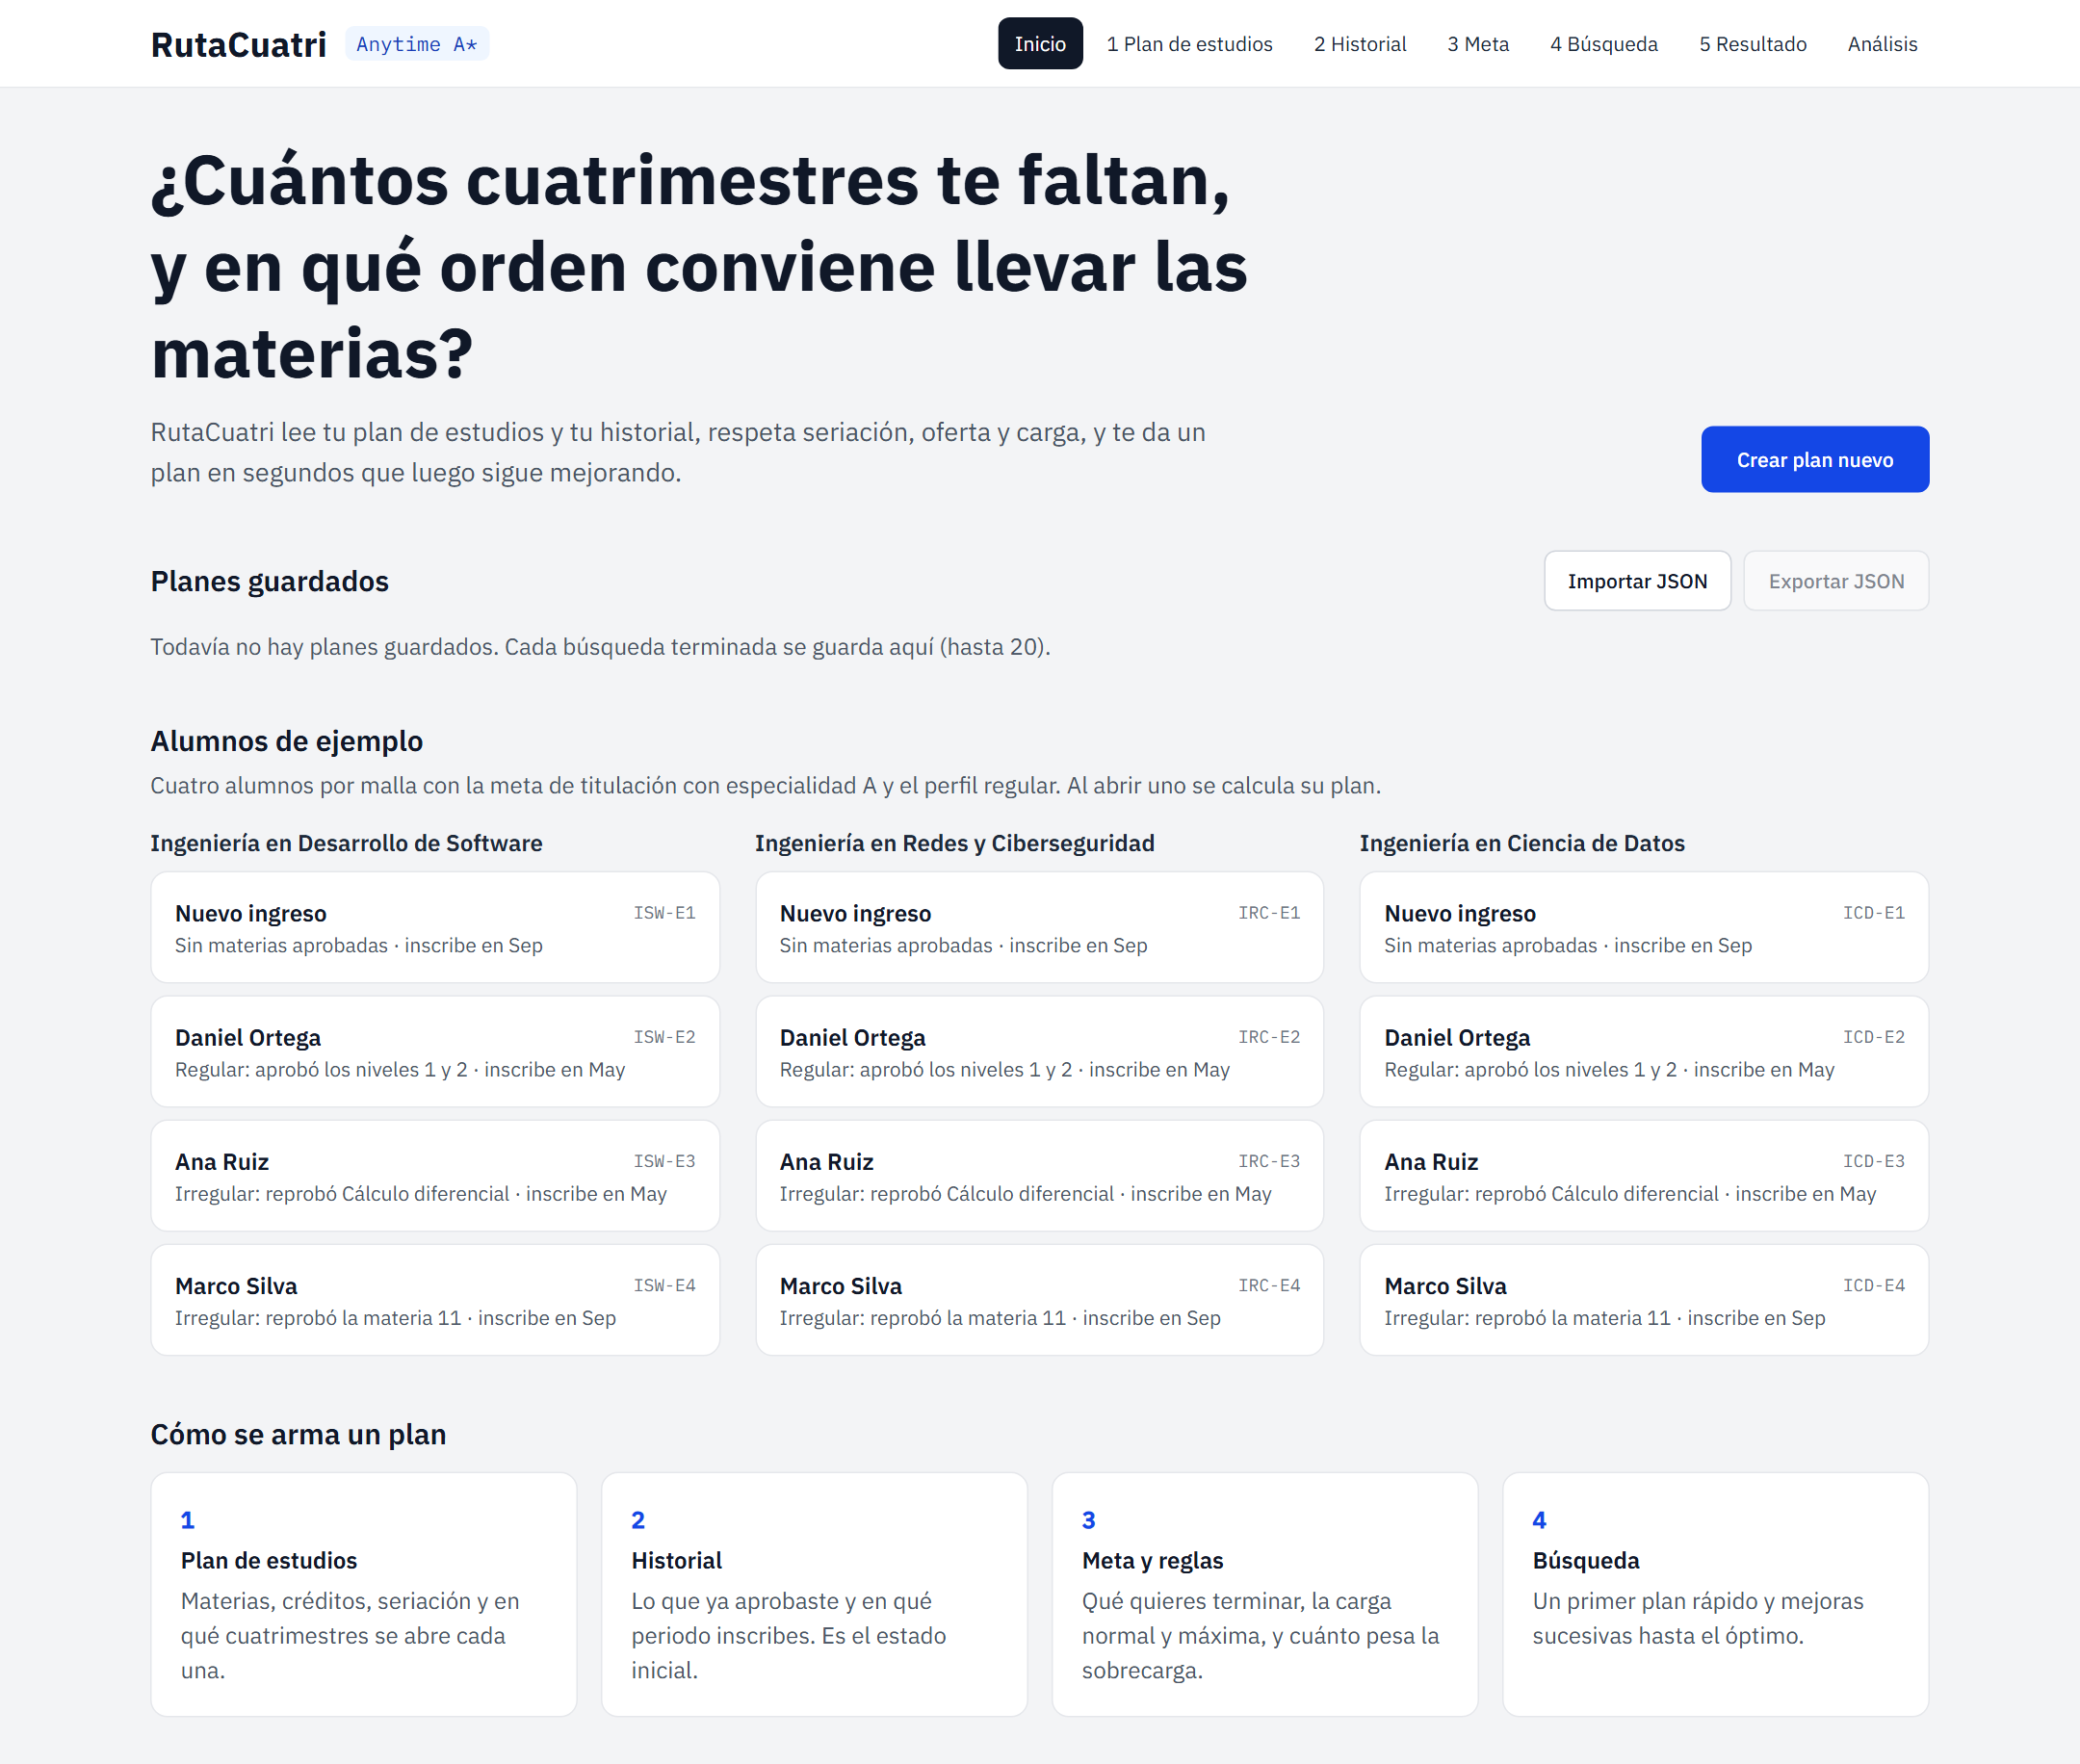
\includegraphics[width=\textwidth]{inicio}
    \caption{Pantalla de inicio con los planes guardados y los alumnos de ejemplo}
    \label{FIG::Inicio}
\end{figure}

\section{Validación del motor}
\label{SEC::Validacion}
El motor se probó contra casos con respuesta conocida, calculados con una implementación de referencia independiente en Python:
\begin{itemize}
    \item \textbf{77 casos:} los 72 escenarios y 5 casos especiales (un ejemplo mínimo de 5 materias, una meta ya cumplida, una materia necesaria sin oferta, una materia más pesada que $C_{max}$ y un plan con un cuatrimestre vacío). El motor da el mismo costo (con tolerancia de $10^{-9}$) y el mismo número de cuatrimestres en los 77.
    \item \textbf{Verificador independiente:} una función aparte, que trabaja con claves y no con máscaras ni con funciones del motor, revisa cada plan (prerrequisitos, oferta, $C_{max}$, $K$ y la estadía sola) y recalcula su costo.
    \item \textbf{Garantía:} en cada pasada se comprueba $\text{costo} \leq H \cdot C^*$.
    \item \textbf{Propiedades en 200 mallas al azar} de 8 a 11 materias: el costo con poda es igual al costo sin poda, $h$ nunca supera el costo real y $h(A) \leq c(S) + h(A \cup S)$ en cada transición.
    \item \textbf{Flujos en el navegador} con Playwright: el plan de Ana Ruiz, el caso sin plan, Detener en menos de un segundo y la vista de celular sin desplazamiento horizontal.
\end{itemize}
A estas se suman pruebas de las funciones de la interfaz, como quitar materias de la malla limpiando la seriación, el historial y la meta. En total son 100 pruebas unitarias y 4 de extremo a extremo, todas aprobadas.
\clearpage
\chapter{Resultados}
\label{CAP::Resultados}
Se presentan cuatro casos de ejecución desde la interfaz y, después, los cuatro experimentos que miden el método. Los tres primeros casos resuelven problemas con mallas, estados iniciales, metas y perfiles distintos; el cuarto muestra cómo el sistema detecta una meta imposible. Todos los tiempos se midieron en un equipo con procesador Intel Core i5-13420H, 16 GB de memoria y Node 22.

\section{Caso 1: Ana Ruiz, alumna irregular}

\subsection{Descripción}
Ana Ruiz estudia Ingeniería en Desarrollo de Software (ISW). Aprobó siete materias de los dos primeros niveles, reprobó Cálculo diferencial (ISW01) y su siguiente inscripción es en mayo. Quiere saber en cuántos cuatrimestres termina la carrera con la especialidad A si lleva la carga regular. El caso no es trivial porque Cálculo diferencial encabeza la cadena más larga que le falta, ISW01 $\to$ ISW06 $\to$ ISW12 $\to$ ISW28, y varias materias de los niveles 3 a 5 solo se abren en dos periodos.

\subsection{Estado inicial y meta}
El estado inicial es $(A_0, \text{May})$ con $A_0 = \{$ISW02, ISW03, ISW04, ISW05, ISW07, ISW08, ISW09$\}$. La Figura~\ref{FIG::C1Historial} muestra la pantalla de historial: ISW01 aparece como reprobada, las materias disponibles en mayo tienen borde punteado y el panel derecho muestra $A_0$, $p_0$ y la cota inicial $h = 4$.

\begin{figure}[H]
    \centering
    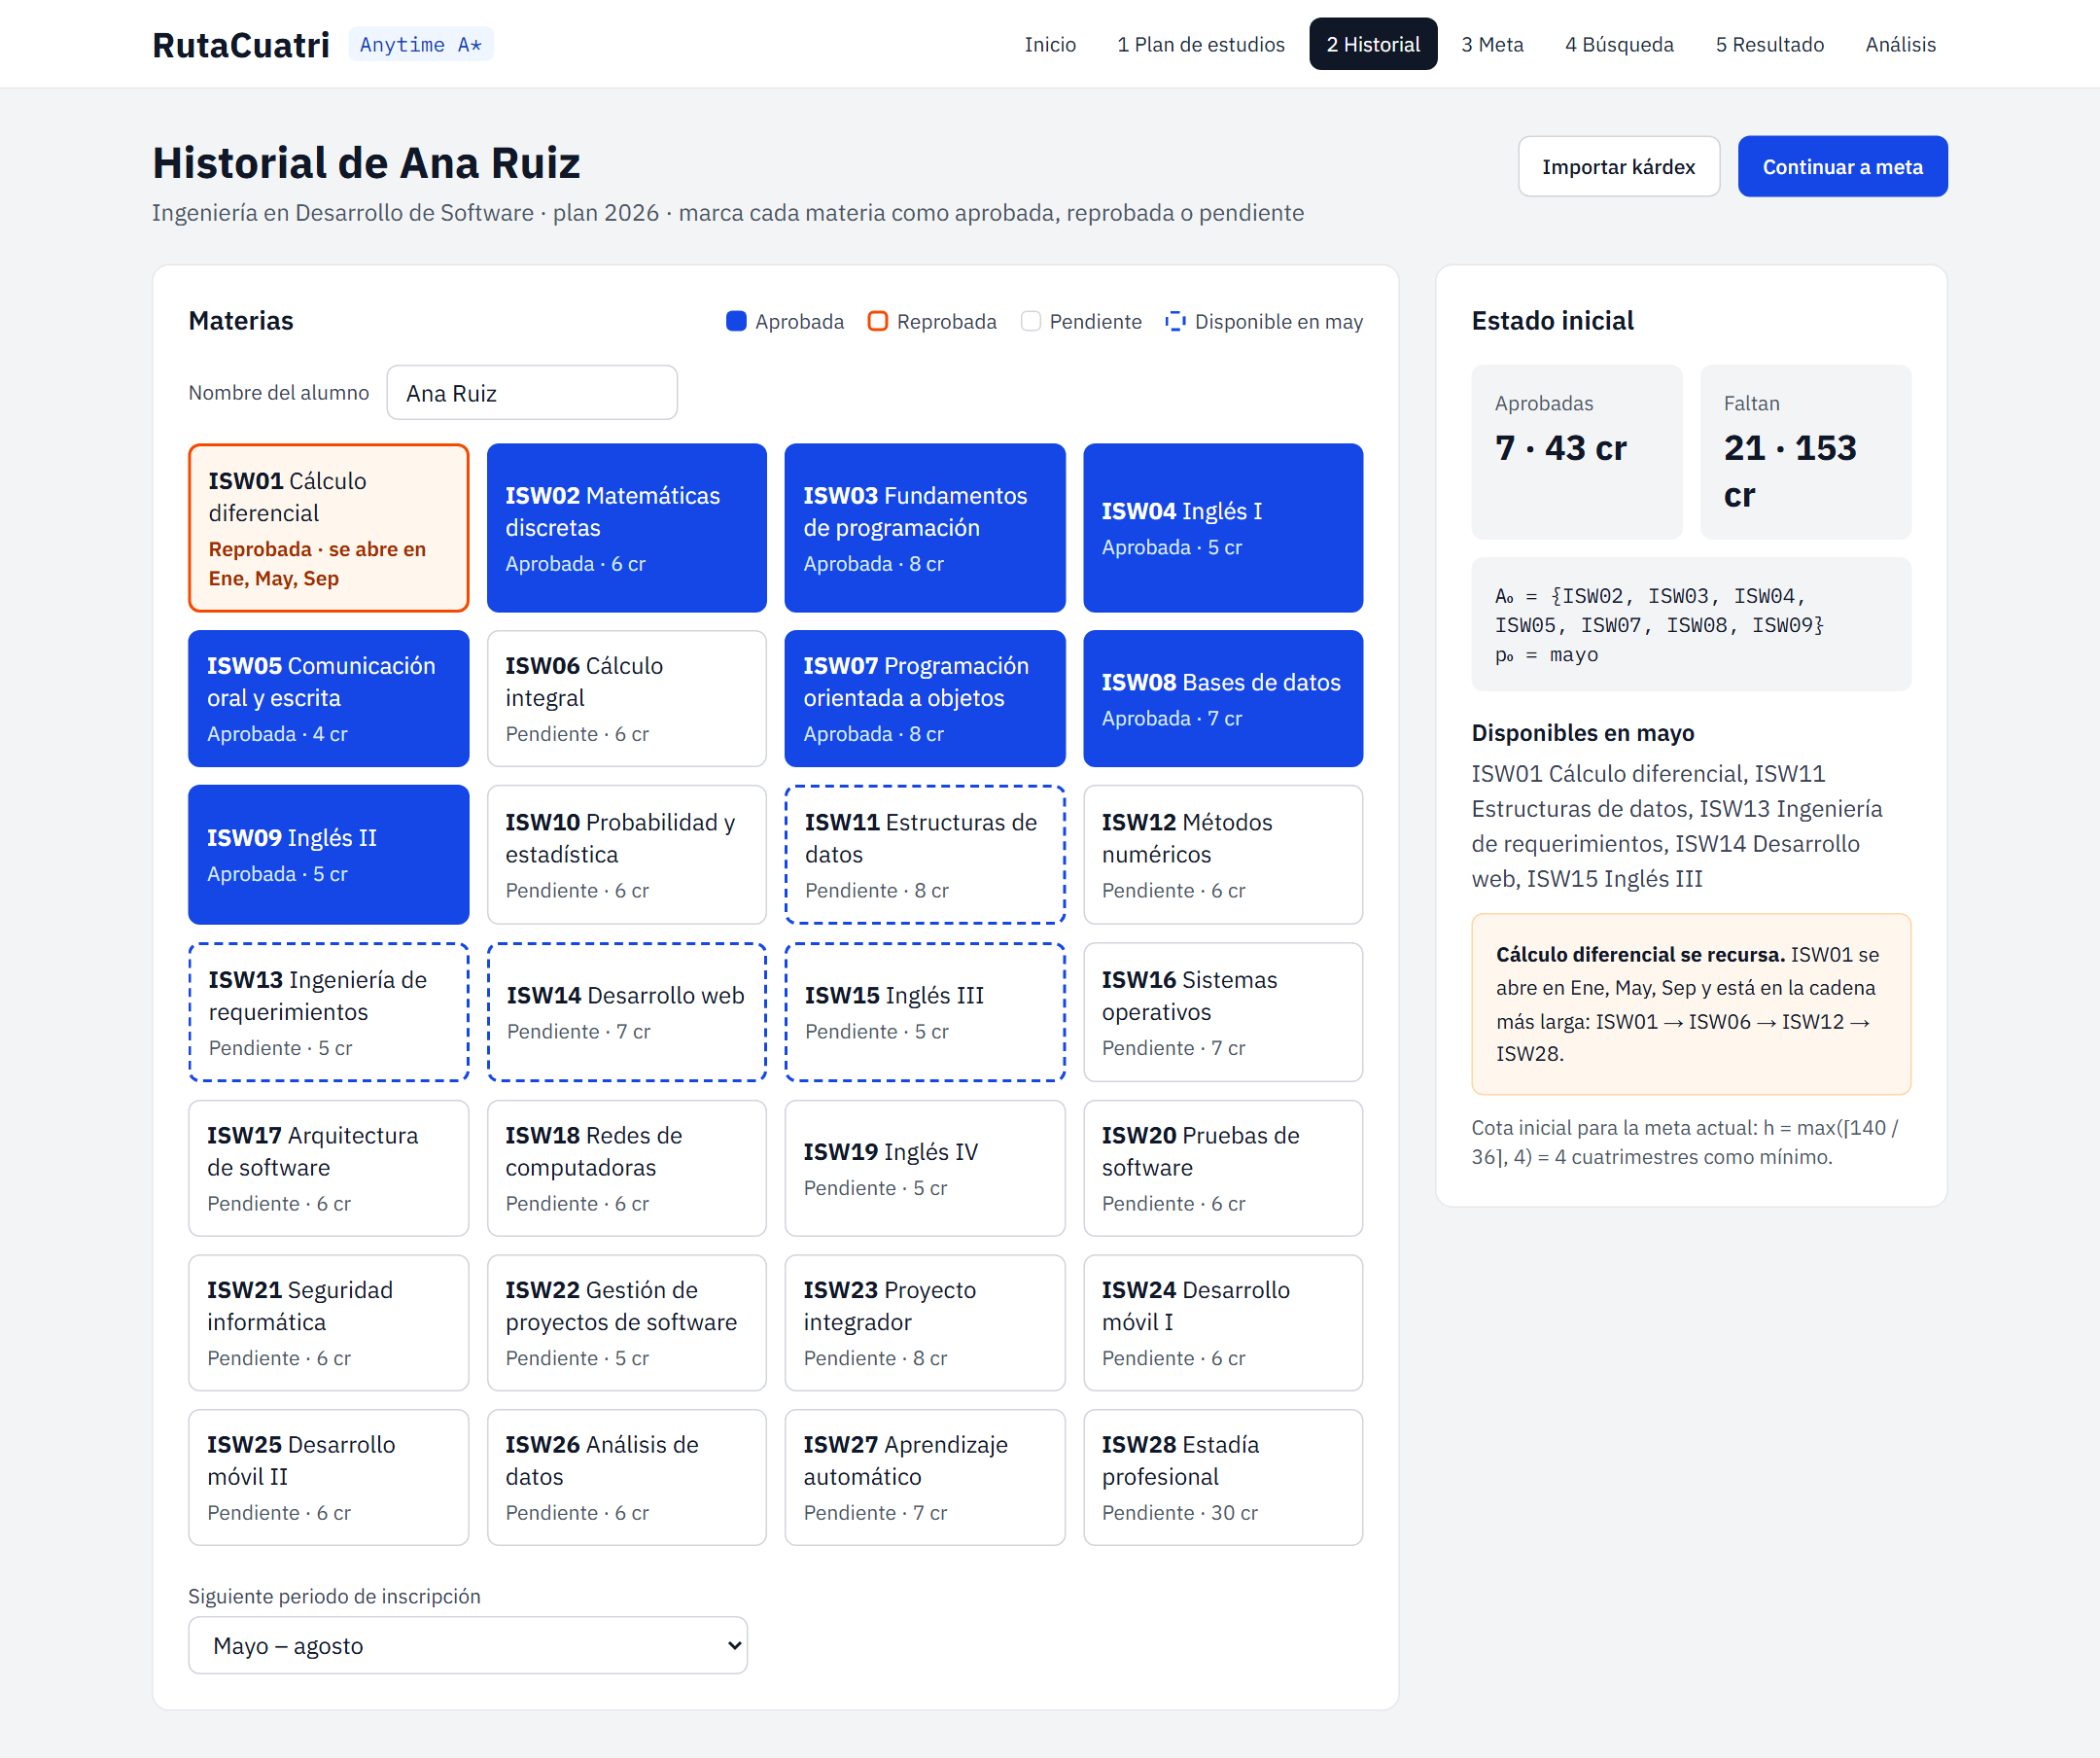
\includegraphics[width=\textwidth,height=0.75\textheight,keepaspectratio]{caso1-historial}
    \caption{Caso 1: historial de Ana Ruiz y estado inicial}
    \label{FIG::C1Historial}
\end{figure}

La meta es la titulación con especialidad A (M1) con el perfil regular ($C_{norm} = 30$, $C_{max} = 36$, $\beta = 0.1$, $K = 7$). La Figura~\ref{FIG::C1Meta} muestra la pantalla de meta y parámetros con el resumen del problema.

\begin{figure}[H]
    \centering
    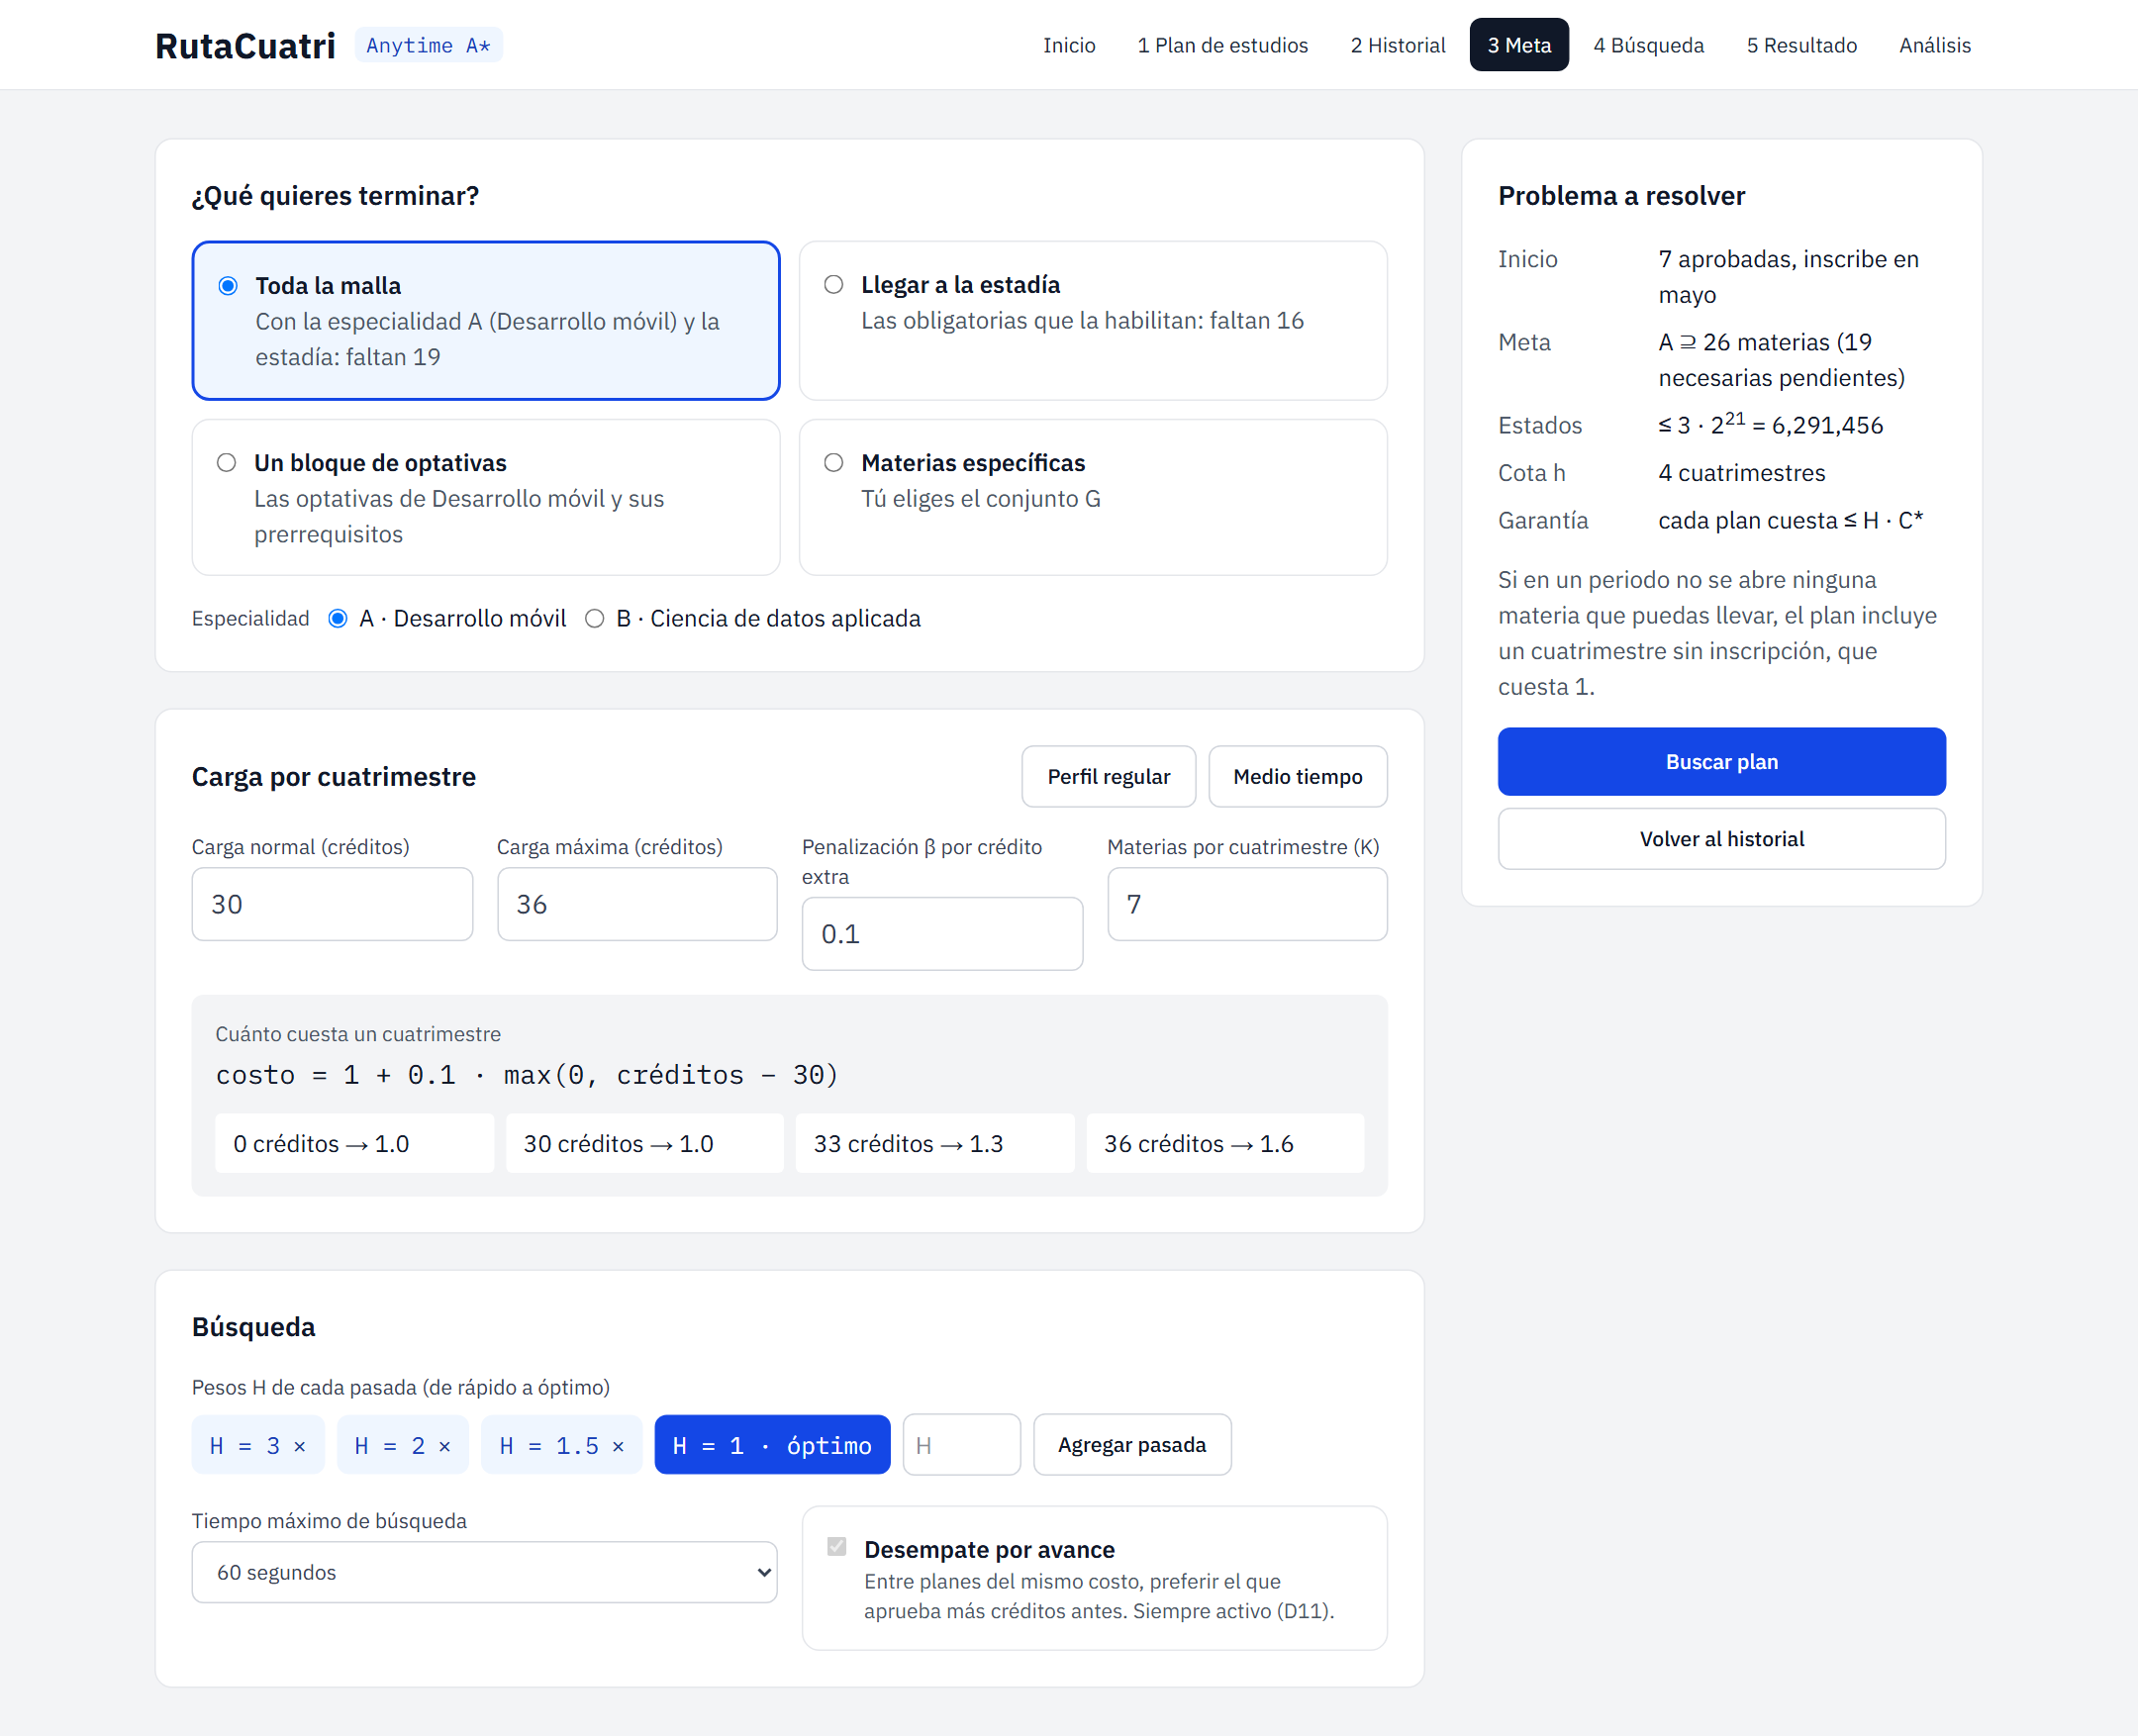
\includegraphics[width=\textwidth,height=0.75\textheight,keepaspectratio]{caso1-meta}
    \caption{Caso 1: meta y parámetros}
    \label{FIG::C1Meta}
\end{figure}

\subsection{Solución}
El plan óptimo tiene 5 cuatrimestres y costo 5.0, sin sobrecarga (Figura~\ref{FIG::C1Resultado}). Ana lleva Cálculo diferencial en su primer cuatrimestre, junto con Estructuras de datos, Ingeniería de requerimientos y Desarrollo web, y termina con la estadía en septiembre del segundo año. El panel derecho explica por qué son 5: la cota es 4 y la oferta obliga a un cuatrimestre más, porque Métodos numéricos (ISW12) solo se abre en mayo y septiembre.

\begin{figure}[H]
    \centering
    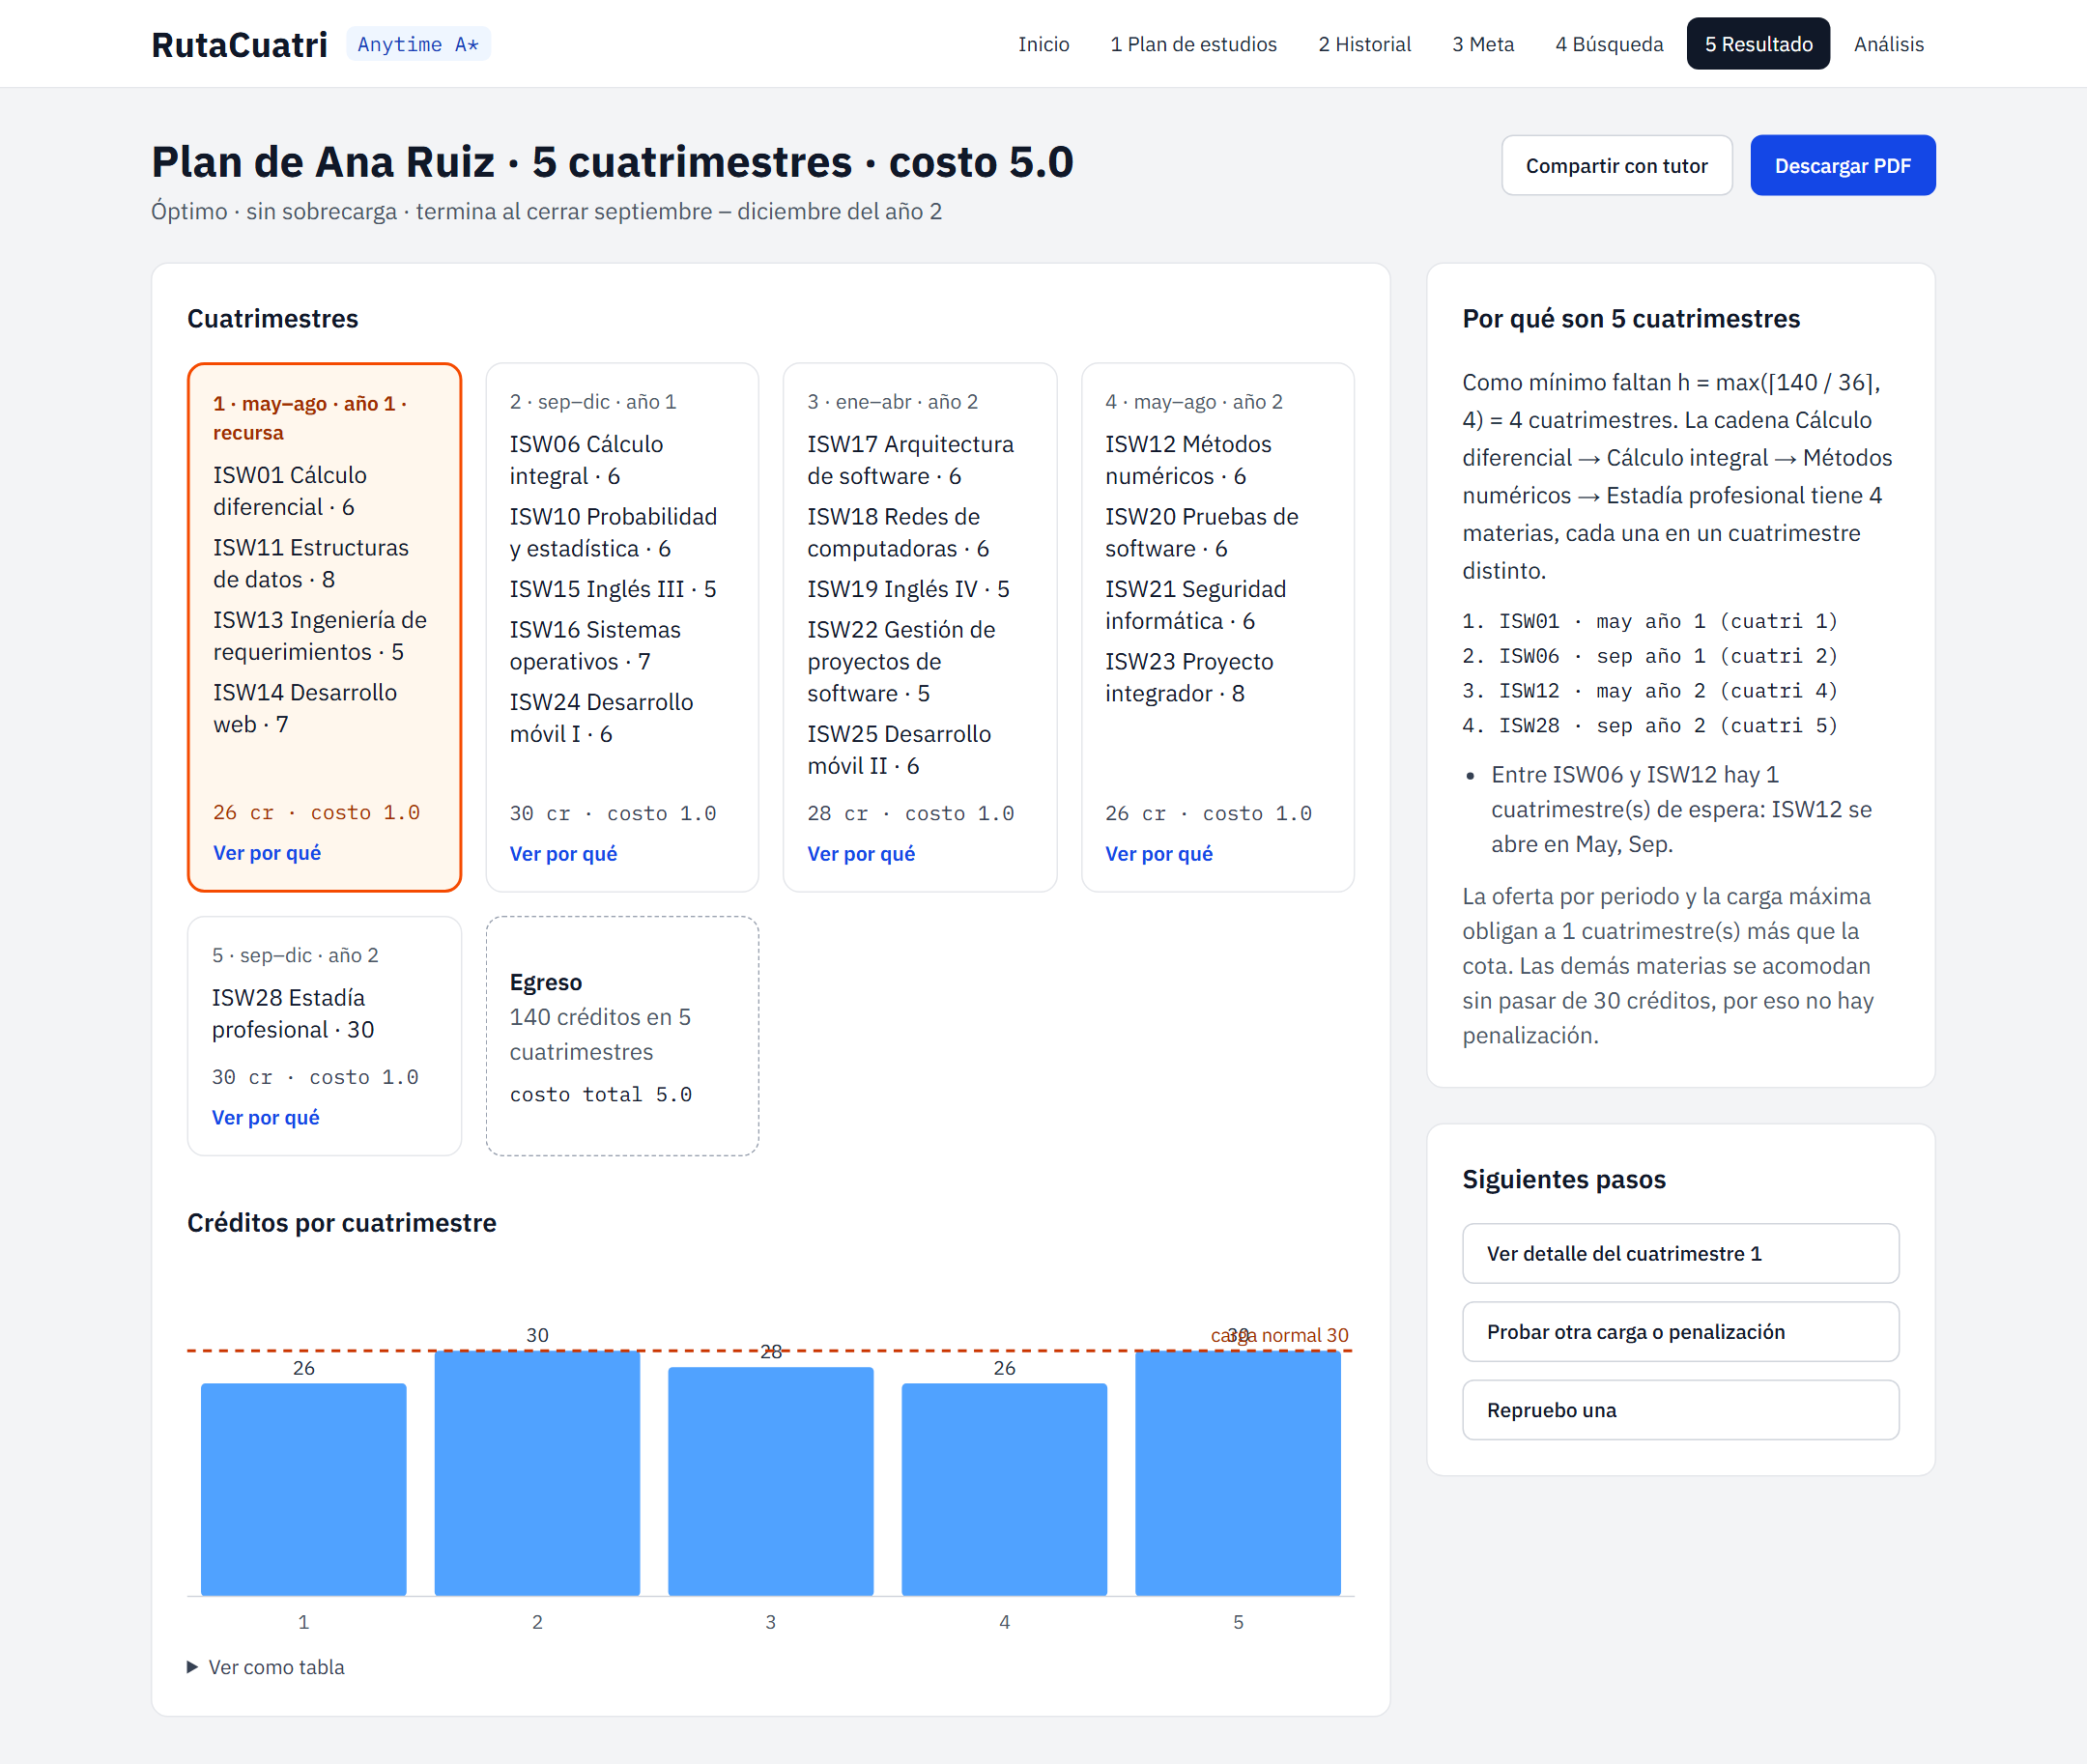
\includegraphics[width=\textwidth,height=0.75\textheight,keepaspectratio]{caso1-resultado}
    \caption{Caso 1: plan óptimo de Ana Ruiz}
    \label{FIG::C1Resultado}
\end{figure}

\subsection{Ejecución}
La búsqueda corre en el Worker y llena la tabla de pasadas (Figura~\ref{FIG::C1Busqueda}). La primera pasada ($H = 3$) encuentra un plan de 7.0 con 8 expansiones; la segunda ($H = 2$) lo mejora a 5.0 con 11; las pasadas con $H = 1.5$ y $H = 1$ expanden solo el estado inicial, porque todos sus sucesores tienen $g + h \geq 5.0$. Eso prueba que 5.0 es el óptimo.

\begin{figure}[H]
    \centering
    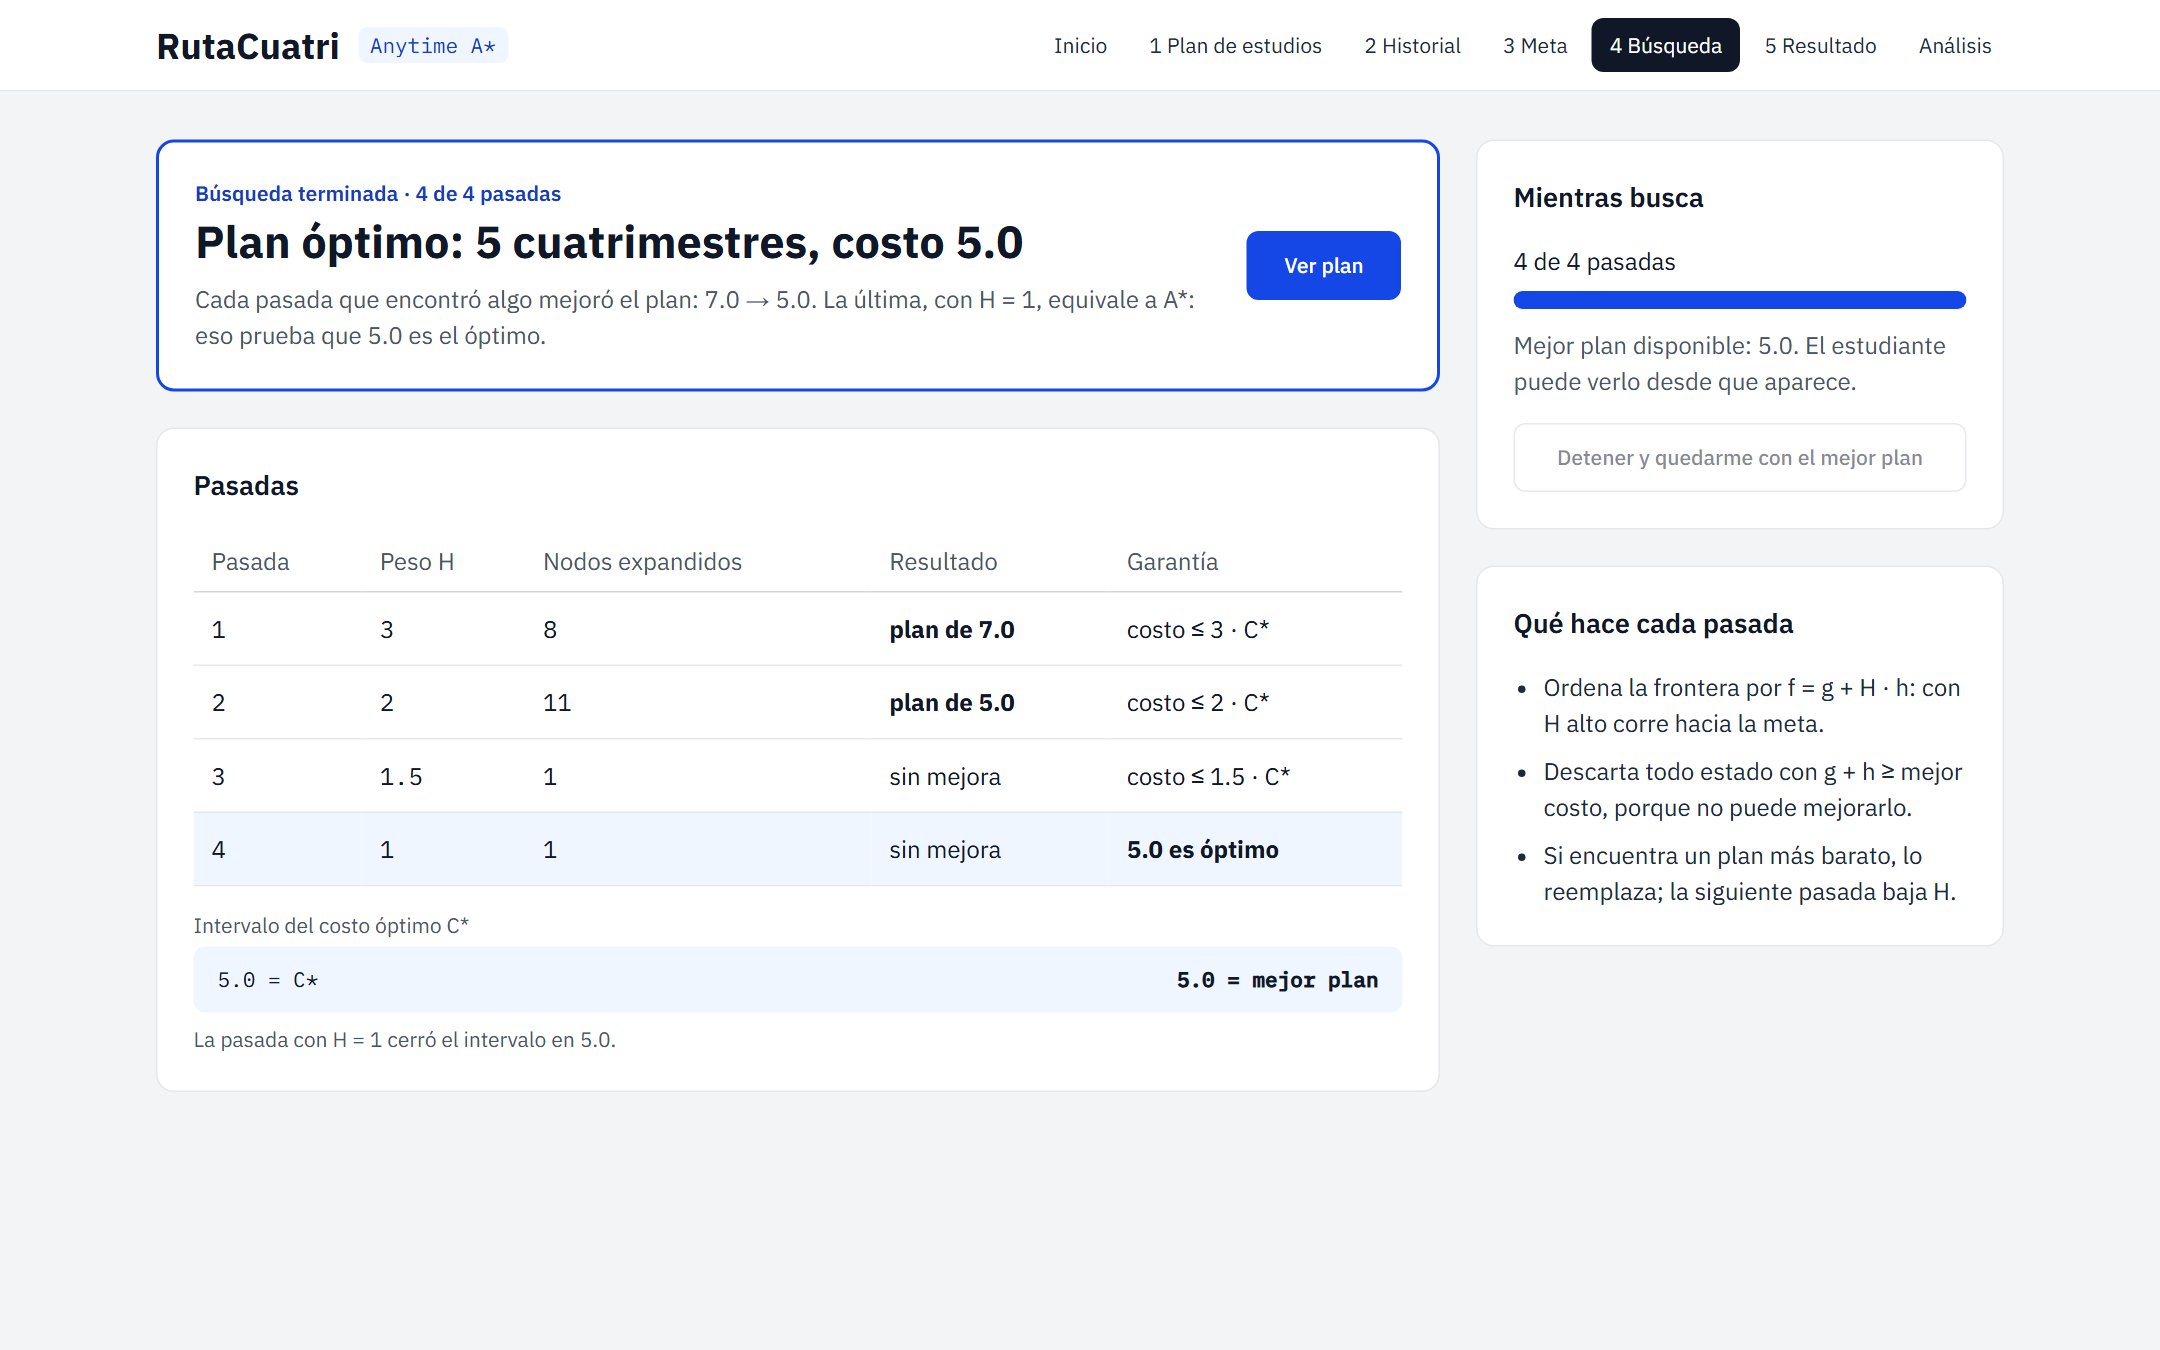
\includegraphics[width=\textwidth,height=0.75\textheight,keepaspectratio]{caso1-busqueda}
    \caption{Caso 1: pasadas de Anytime A*}
    \label{FIG::C1Busqueda}
\end{figure}

La Figura~\ref{FIG::C1Detalle} muestra el detalle del primer cuatrimestre: las materias inscritas y la pospuesta, y las alternativas con su costo total calculado con A* desde el estado que deja cada una (son los sucesores de la Tabla~\ref{TAB::TransicionesAna}). La elegida tiene el menor costo total y el estado $n'$ que deja cumple $f(n') = 1.0 + 4 = 5.0 \leq 5.0$.

\begin{figure}[H]
    \centering
    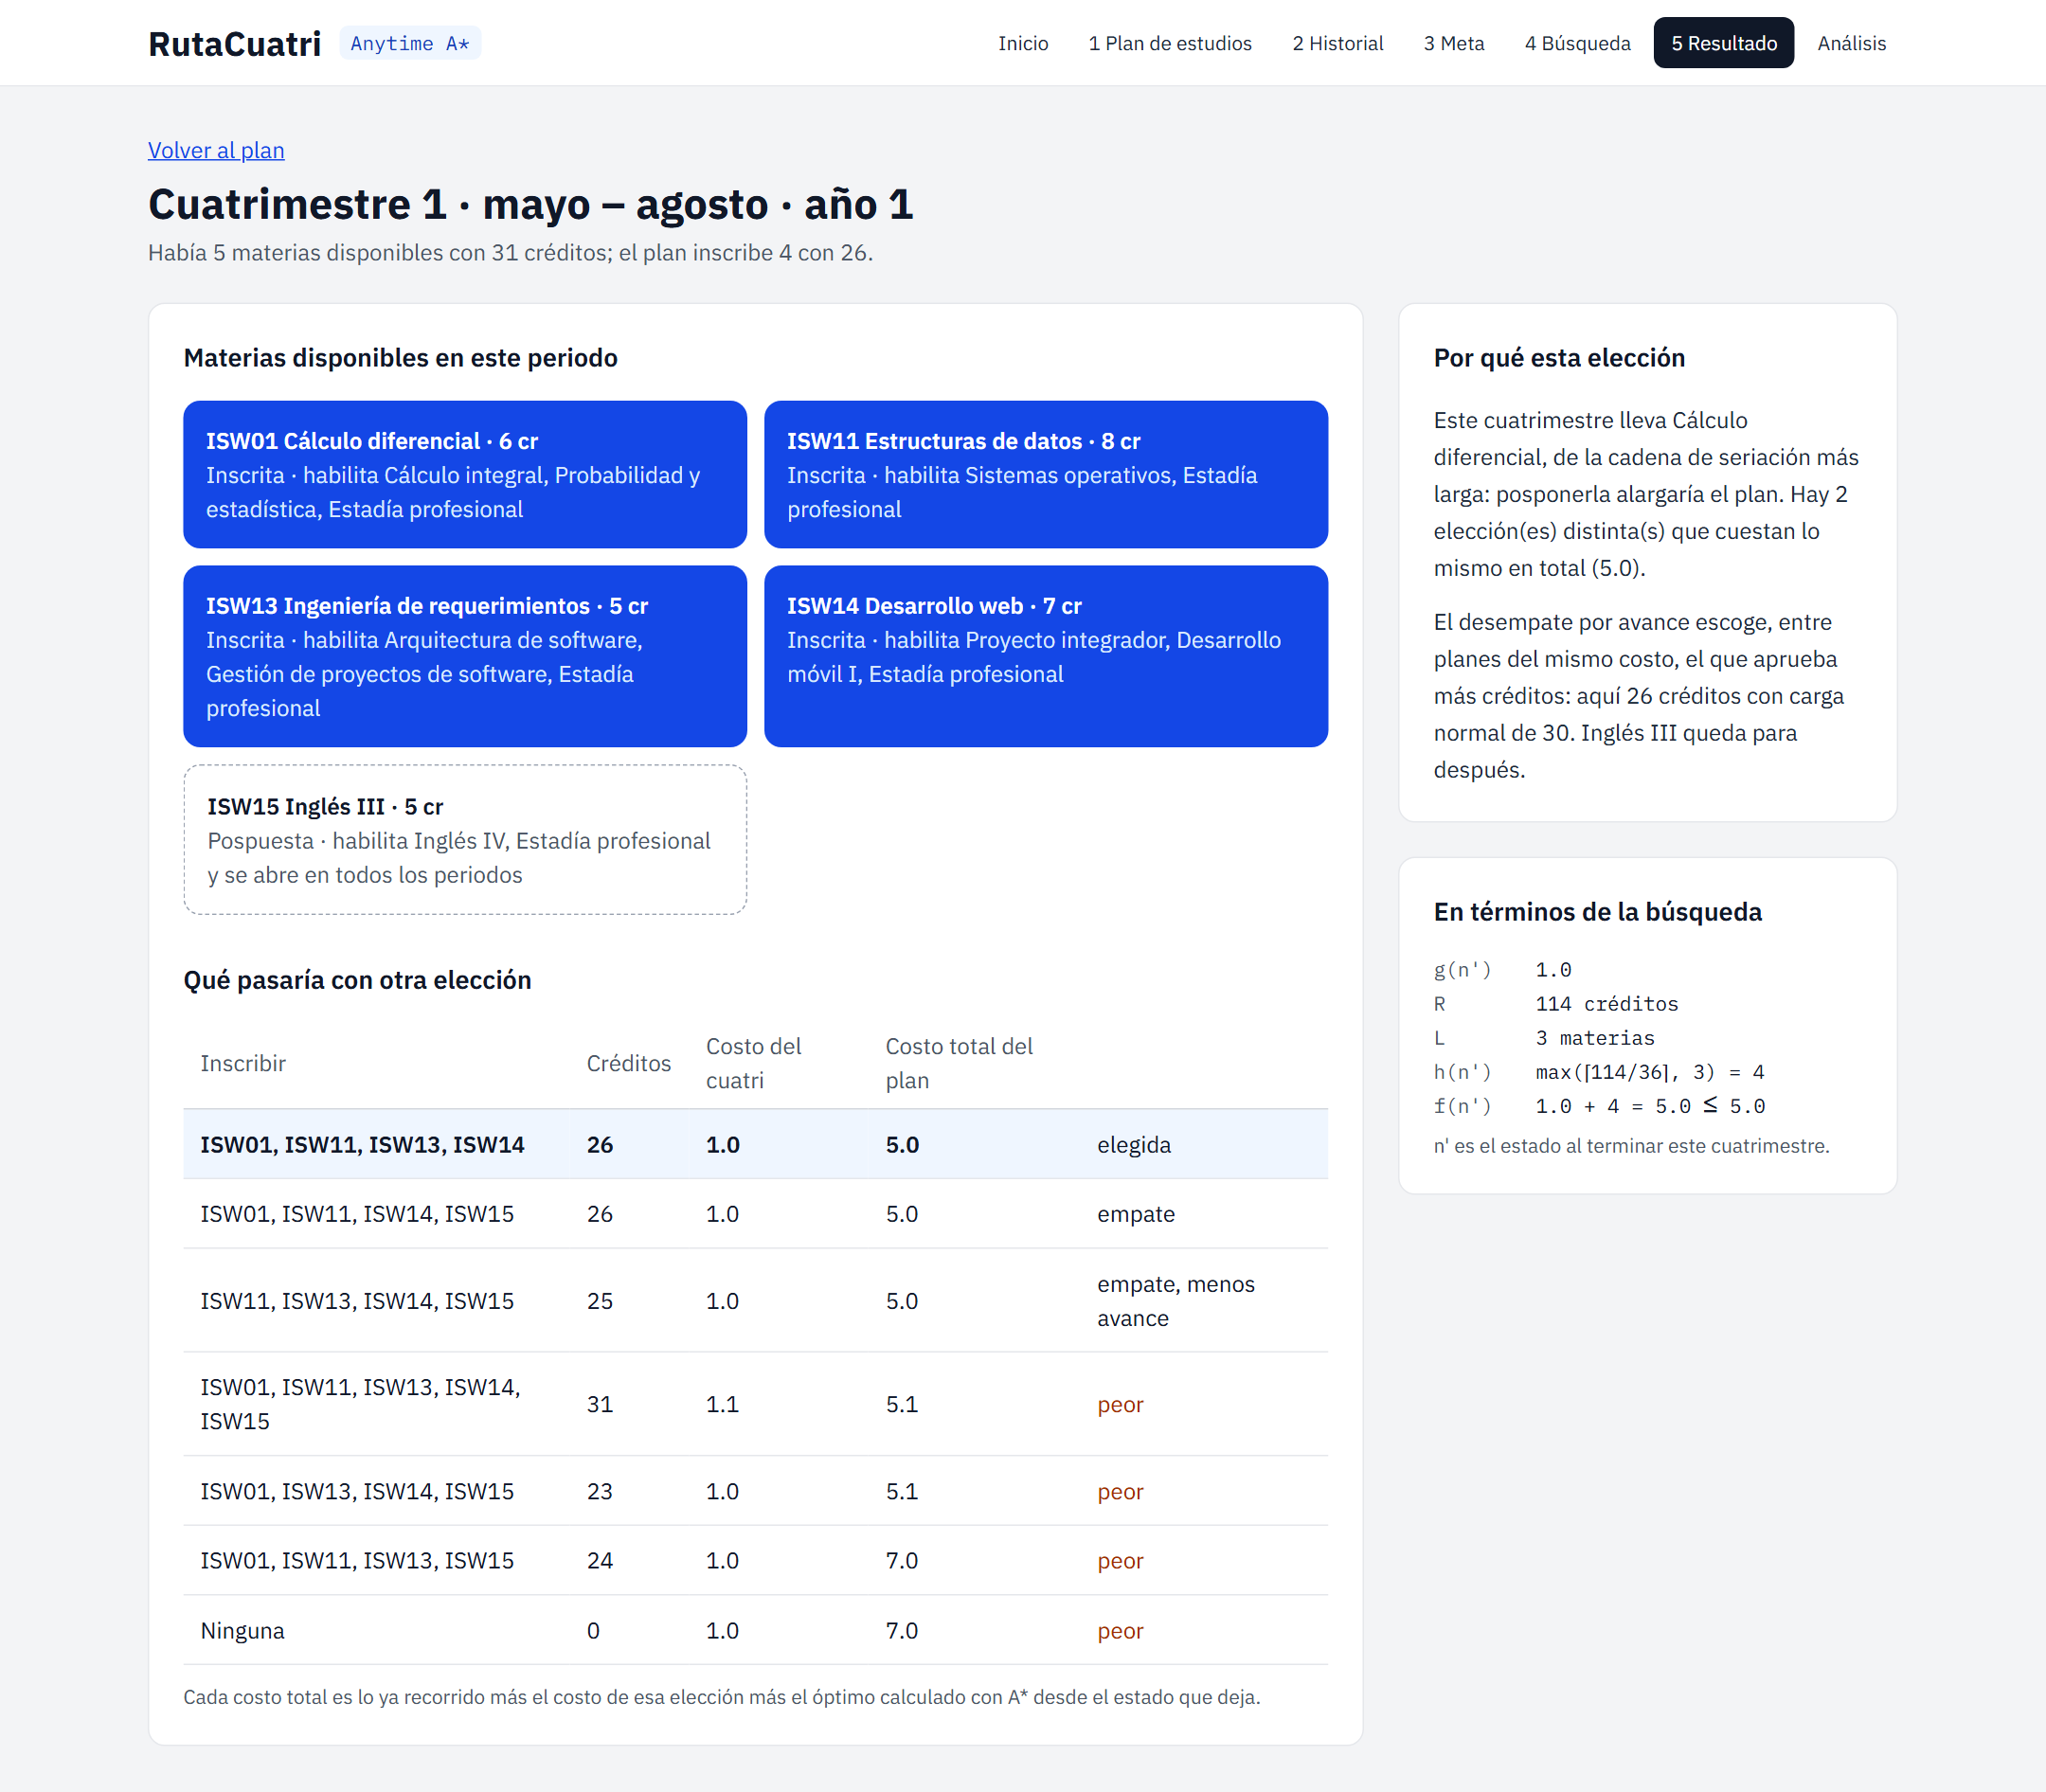
\includegraphics[width=\textwidth,height=0.8\textheight,keepaspectratio]{caso1-detalle}
    \caption{Caso 1: detalle del primer cuatrimestre y sus alternativas}
    \label{FIG::C1Detalle}
\end{figure}

Por último, la Figura~\ref{FIG::C1Celular} muestra la vista de celular con la opción ``Repruebo una''. Si Ana vuelve a reprobar Cálculo diferencial en su primer cuatrimestre, el sistema marca las otras tres materias como aprobadas, deja Cálculo diferencial como reprobada y vuelve a buscar desde septiembre: le quedan 4 cuatrimestres con costo 4.0.

\begin{figure}[H]
    \centering
    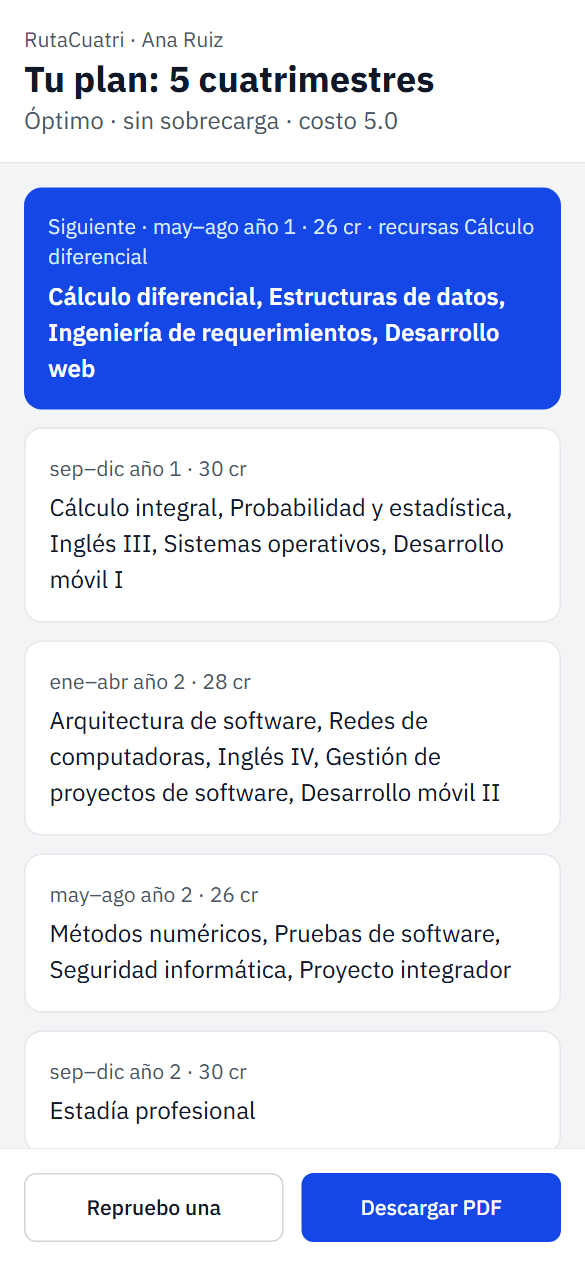
\includegraphics[width=0.31\textwidth]{caso1-celular}\hfill
    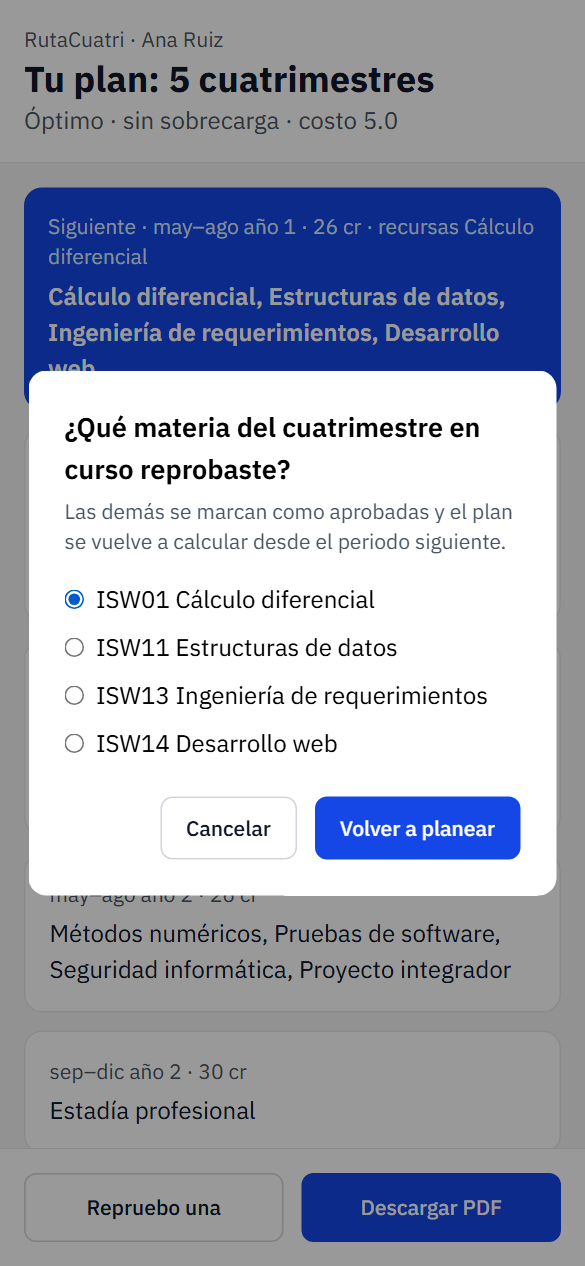
\includegraphics[width=0.31\textwidth]{caso1-repruebo}\hfill
    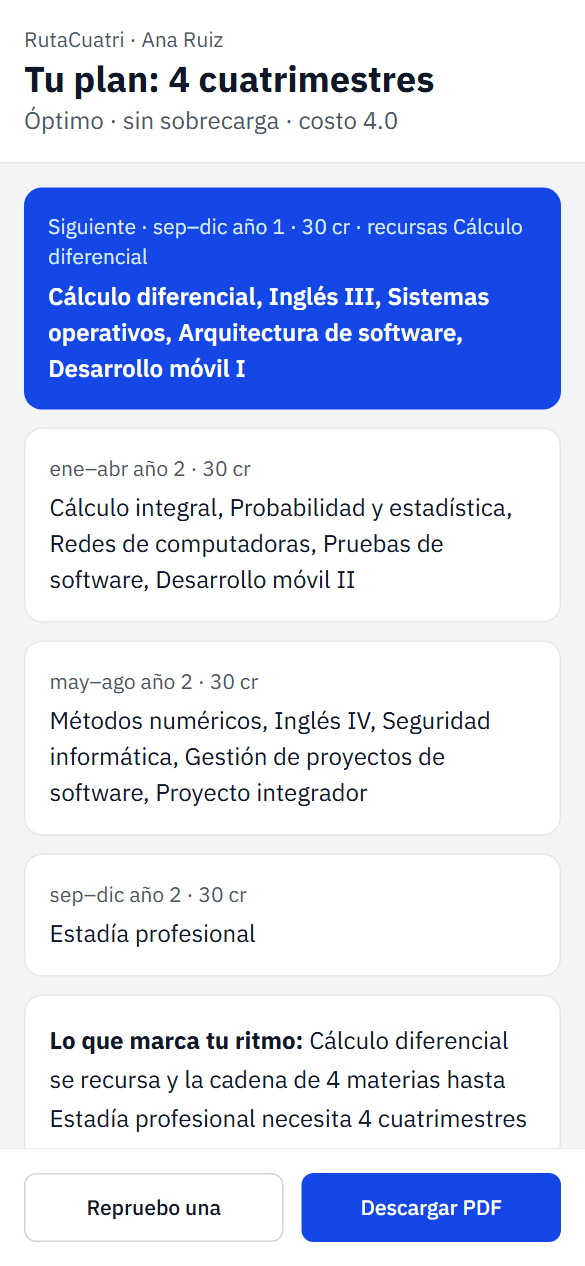
\includegraphics[width=0.31\textwidth]{caso1-replaneado}
    \caption{Caso 1: vista de celular, ``Repruebo una'' y plan recalculado}
    \label{FIG::C1Celular}
\end{figure}

\subsection{Comentarios}
Con la carga regular, Ana termina en septiembre del segundo año, en 5 cuatrimestres: uno más que la cota, por la espera de Métodos numéricos. La cadena ISW01 $\to$ ISW06 $\to$ ISW12 $\to$ ISW28 marca el ritmo, y por eso el plan inscribe Cálculo diferencial en el primer cuatrimestre. Incluso si lo reprueba otra vez, el plan recalculado sigue terminando en el mismo septiembre. La primera pasada dio un plan 40\% más caro que el óptimo (7.0 contra 5.0), lejos de su garantía de $3 \cdot C^*$, y la segunda ya llegó al óptimo.

\section{Caso 2: nuevo ingreso con carga de medio tiempo}

\subsection{Descripción}
Un estudiante de nuevo ingreso de ISW trabaja y solo puede llevar carga de medio tiempo. Quiere terminar toda la carrera con la especialidad A. Es el escenario más difícil de los 72: las 26 materias son necesarias y, con $C_{norm} = 24$, el estudiante ya no cabe en un nivel por cuatrimestre, así que la búsqueda tiene que negociar entre cargar de más y alargar la carrera.

\subsection{Estado inicial y meta}
El estado inicial es $(\emptyset, \text{Sep})$ y la meta es M1. En la pantalla de meta se eligió el perfil de medio tiempo ($C_{norm} = 24$, $C_{max} = 30$); el resumen muestra hasta $3 \cdot 2^{28} = 805{,}306{,}368$ estados y una cota inicial de 7 cuatrimestres (Figura~\ref{FIG::C2Meta}).

\begin{figure}[H]
    \centering
    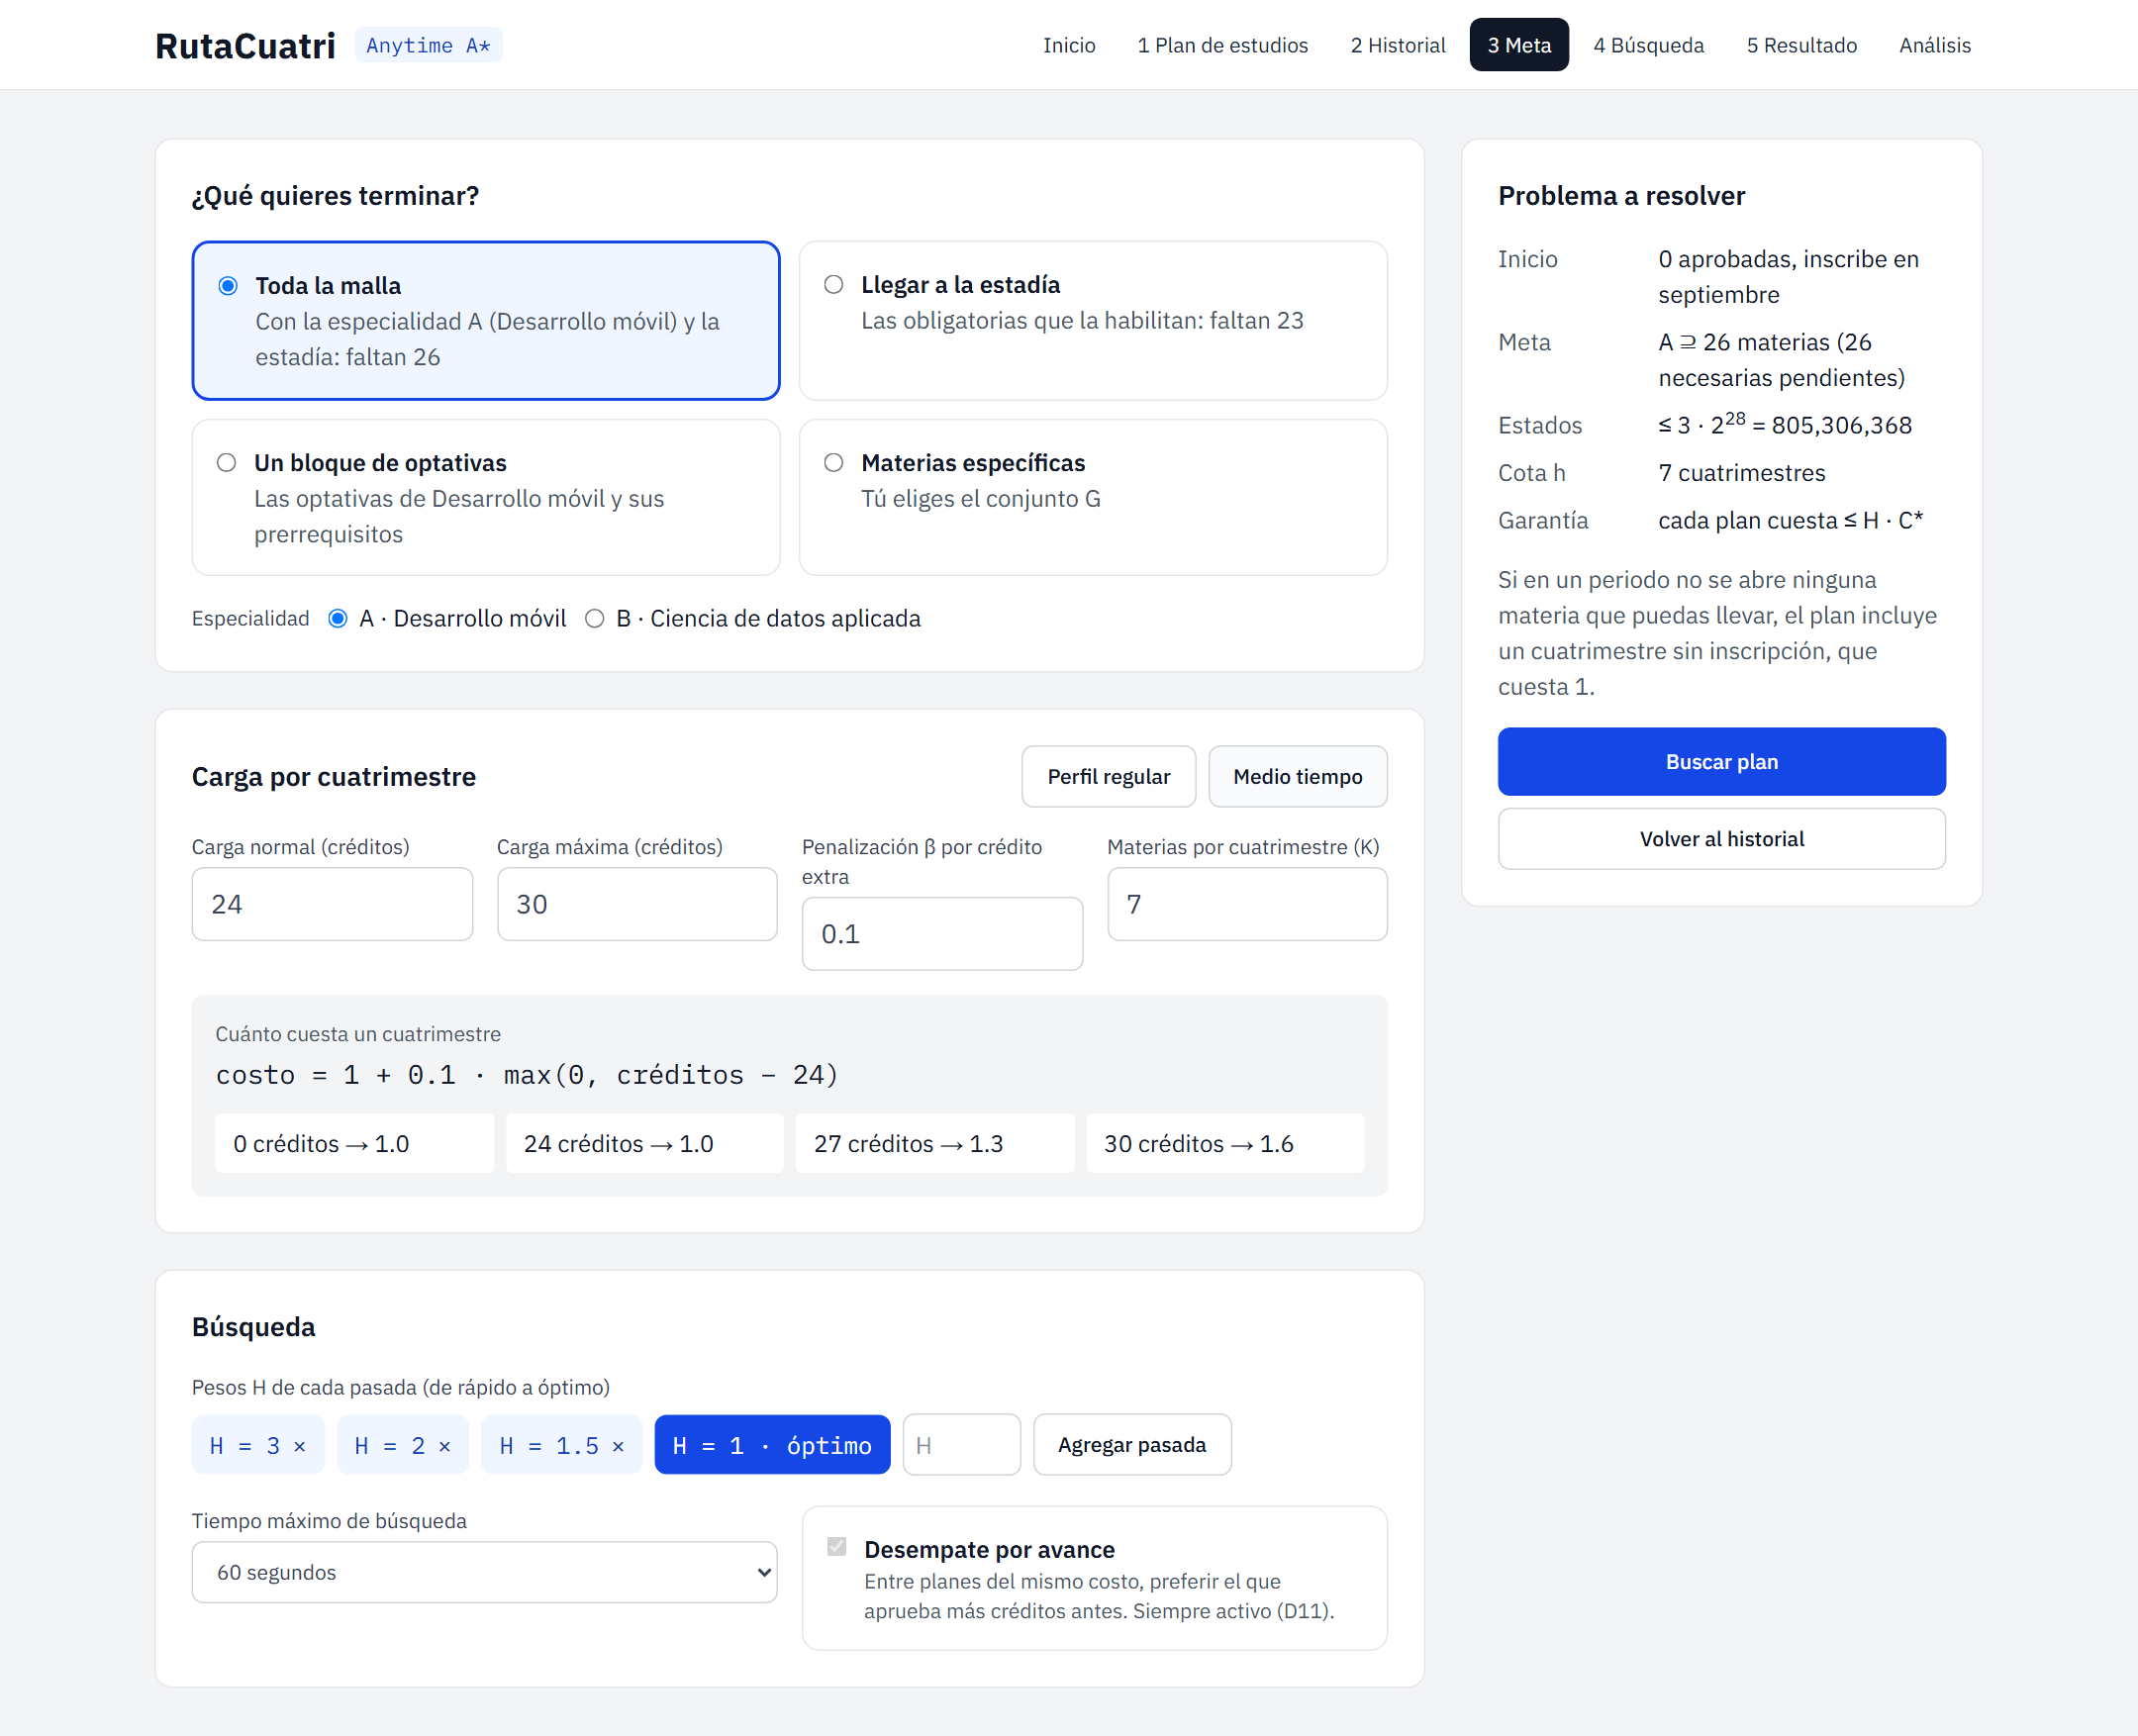
\includegraphics[width=\textwidth,height=0.75\textheight,keepaspectratio]{caso2-meta}
    \caption{Caso 2: meta y perfil de medio tiempo}
    \label{FIG::C2Meta}
\end{figure}

\subsection{Solución}
El plan óptimo tiene 7 cuatrimestres y costo 8.5 (Figura~\ref{FIG::C2Resultado}). Lleva 15 créditos de sobrecarga repartidos en cuatro cuatrimestres; la gráfica de créditos los marca en naranja sobre la línea de la carga normal.

\begin{figure}[H]
    \centering
    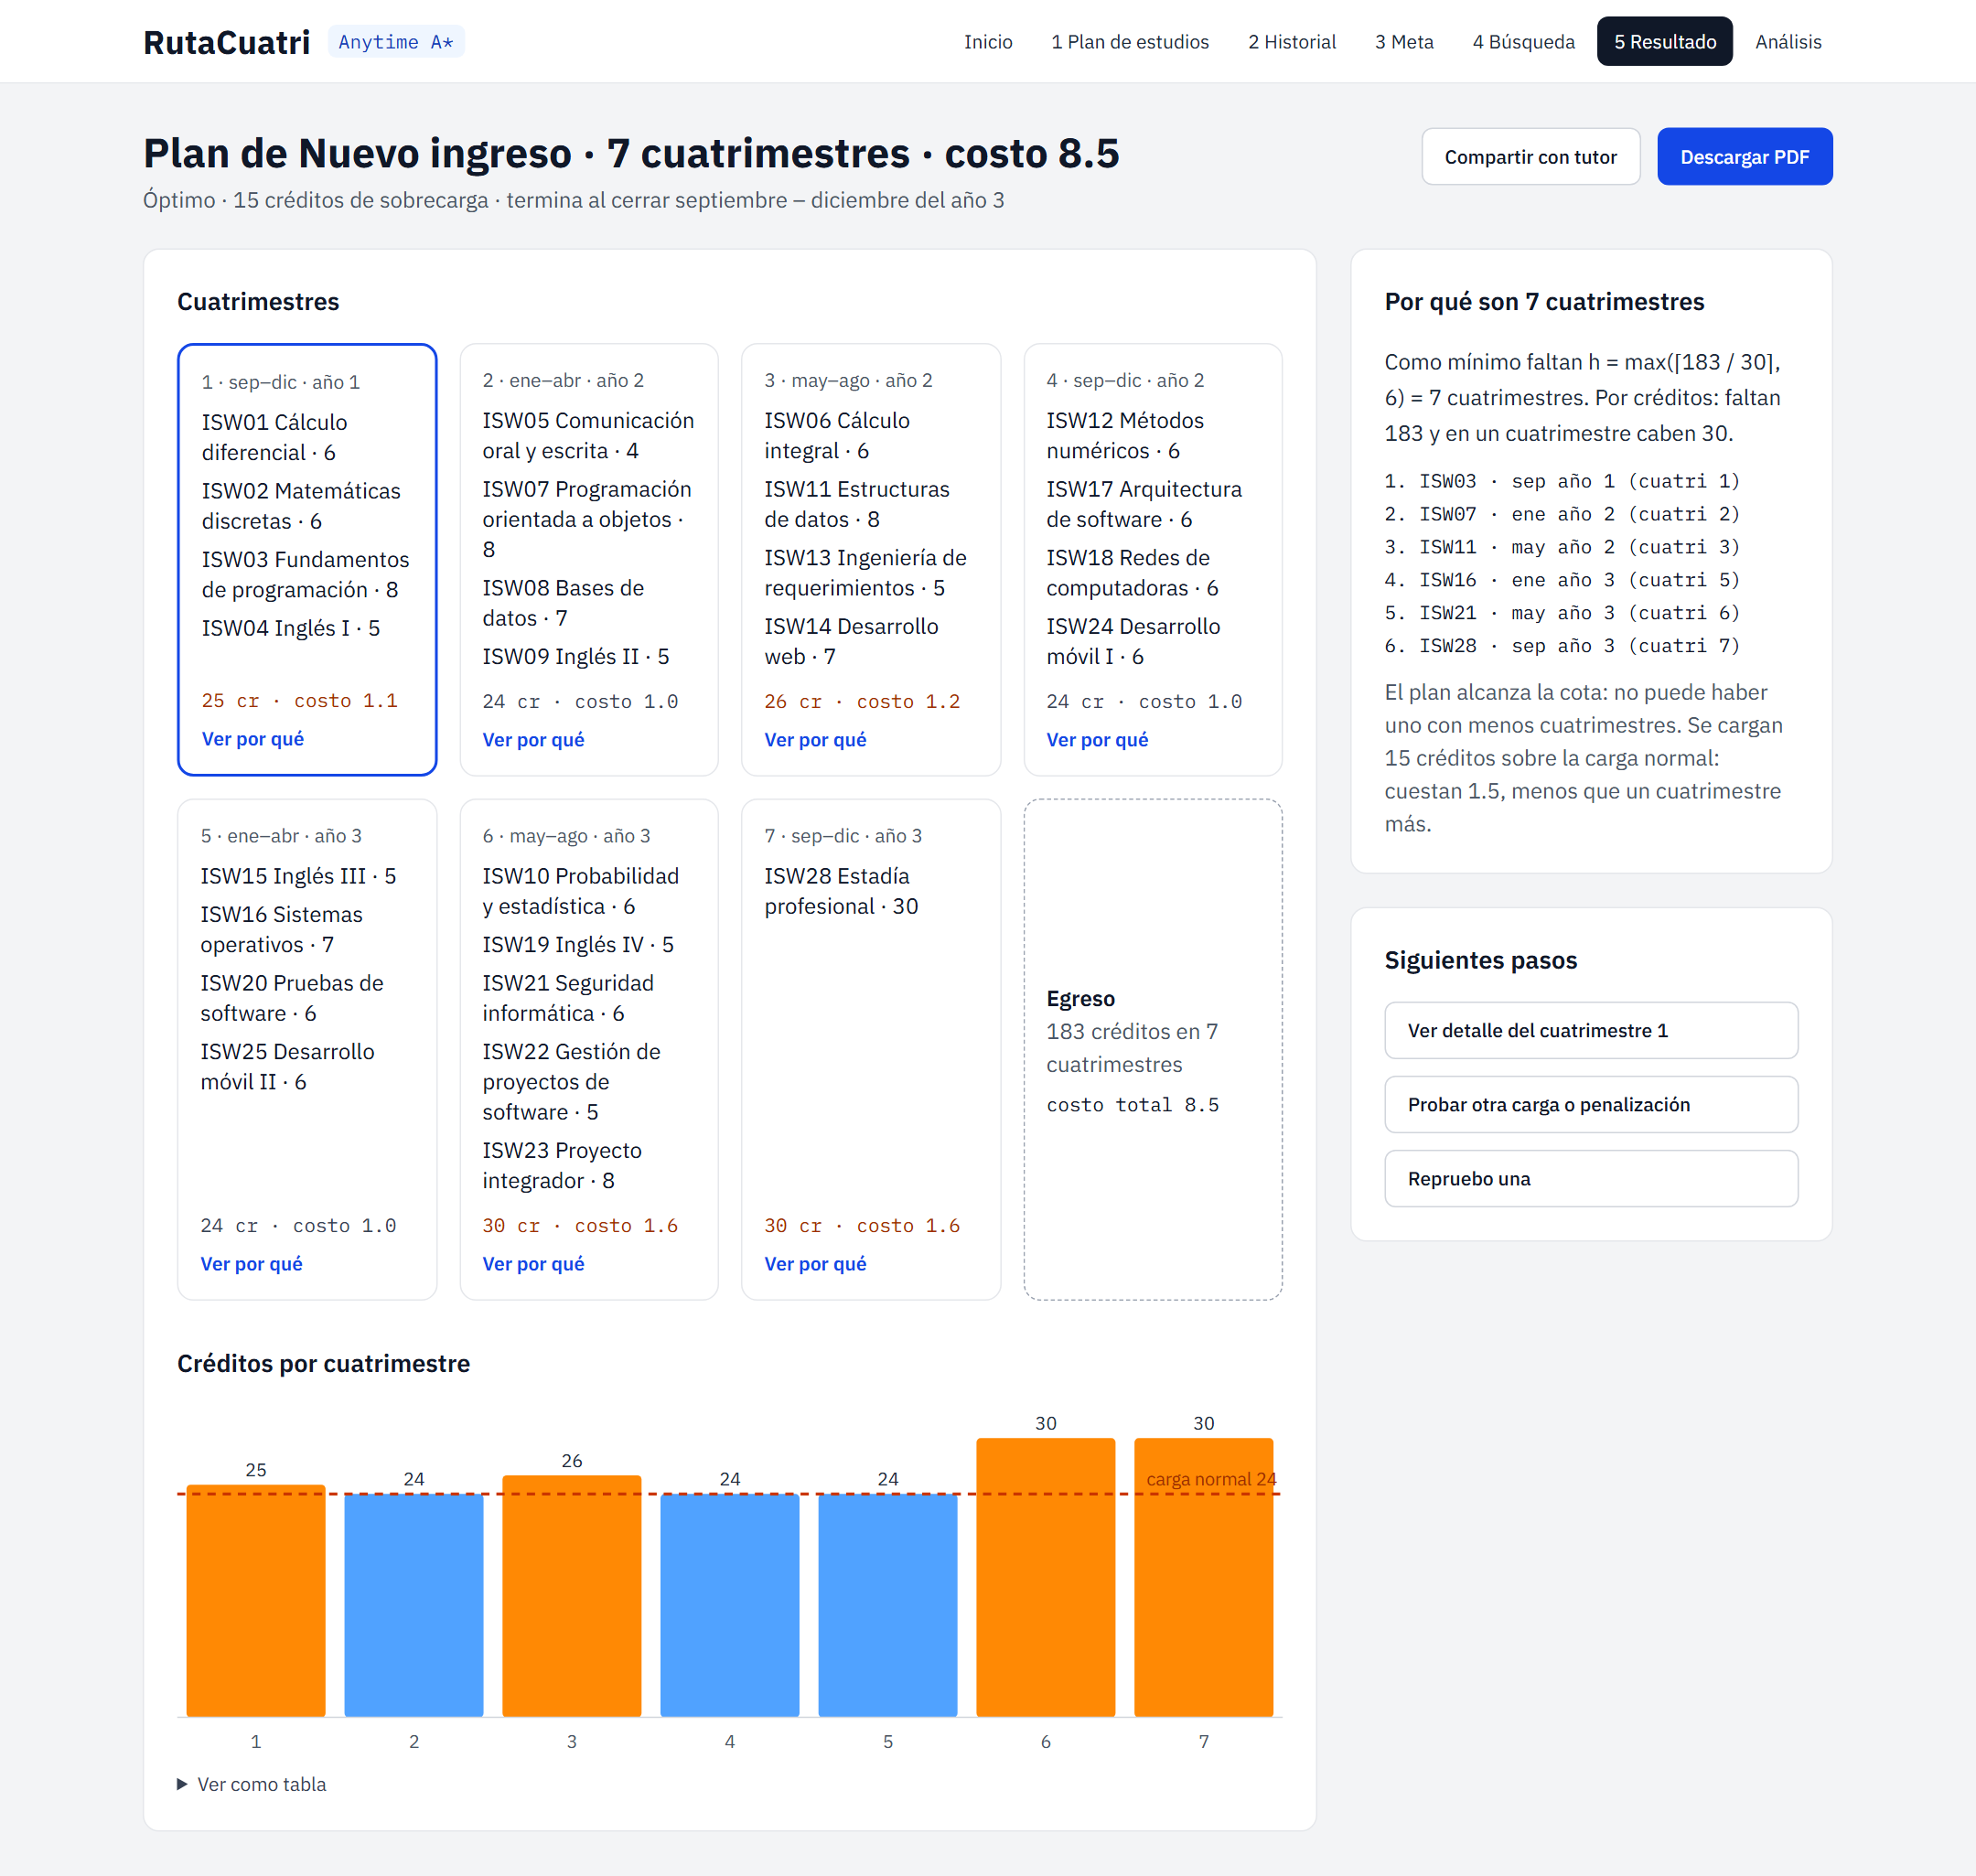
\includegraphics[width=\textwidth,height=0.75\textheight,keepaspectratio]{caso2-resultado}
    \caption{Caso 2: plan óptimo con carga de medio tiempo}
    \label{FIG::C2Resultado}
\end{figure}

\subsection{Ejecución}
Aquí las cuatro pasadas mejoran el plan (Figura~\ref{FIG::C2Busqueda}): 10.0 con 17 expansiones, 9.6 con 22, 8.8 con 77 y 8.5 con 2,918. El primer plan sale en 0.2 ms y el óptimo queda demostrado en 38 ms. Desde la primera pasada el estudiante sabe que el óptimo está entre $h = 7$ y 10.0.

\begin{figure}[H]
    \centering
    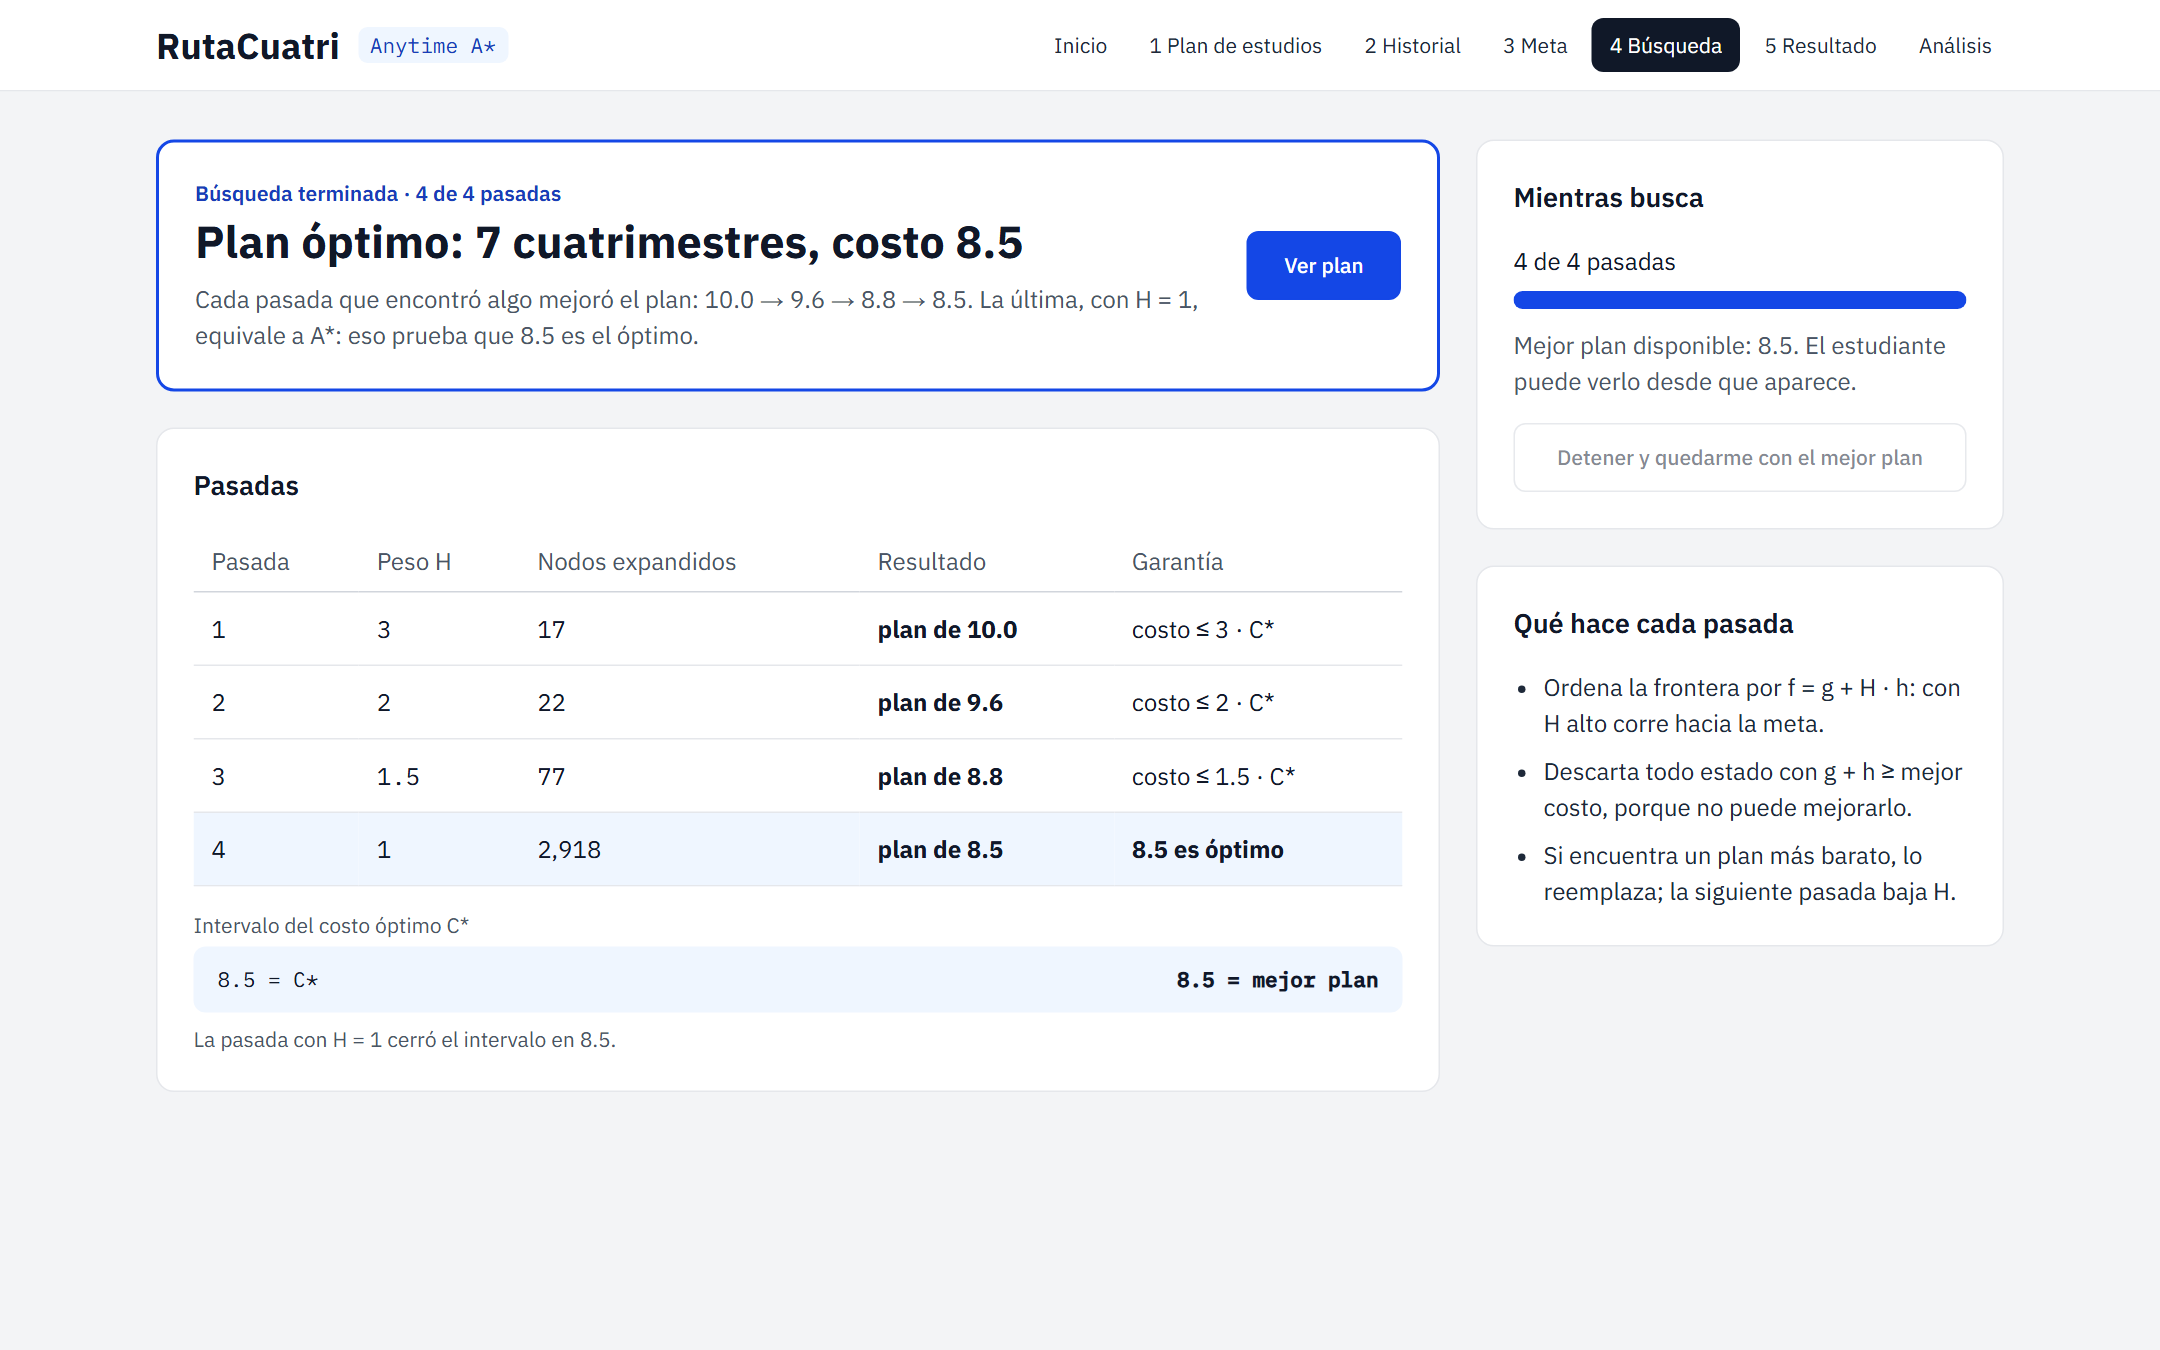
\includegraphics[width=\textwidth,height=0.75\textheight,keepaspectratio]{caso2-busqueda}
    \caption{Caso 2: cada pasada mejora el plan}
    \label{FIG::C2Busqueda}
\end{figure}

\subsection{Comentarios}
Es el caso en que Anytime A* se distingue: el primer plan cuesta 18\% más que el óptimo y llega con menos del 1\% de las expansiones de A*. La pasada final hace el 96\% del trabajo, que es el precio de demostrar el óptimo. El plan muestra que con medio tiempo conviene cargar de más en algunos cuatrimestres: 15 créditos extra cuestan 1.5, menos que los cuatrimestres adicionales que harían falta para no cargar nada.

\section{Caso 3: llegar a la estadía en Redes y Ciberseguridad}

\subsection{Descripción}
Un estudiante de nuevo ingreso de Ingeniería en Redes y Ciberseguridad (IRC) con carga de medio tiempo no quiere todavía la especialidad: quiere saber cuándo puede empezar la estadía. El caso cambia la malla, la meta y el perfil respecto a los anteriores.

\subsection{Estado inicial y meta}
El estado inicial es $(\emptyset, \text{Sep})$ en la malla IRC y la meta es M2, las 23 obligatorias. La cota inicial es $h = \max(\lceil 142/30 \rceil, 5) = 5$, por la cadena IRC03 $\to$ IRC08 $\to$ IRC11 $\to$ IRC16 $\to$ IRC20 (Figura~\ref{FIG::C3Meta}).

\begin{figure}[H]
    \centering
    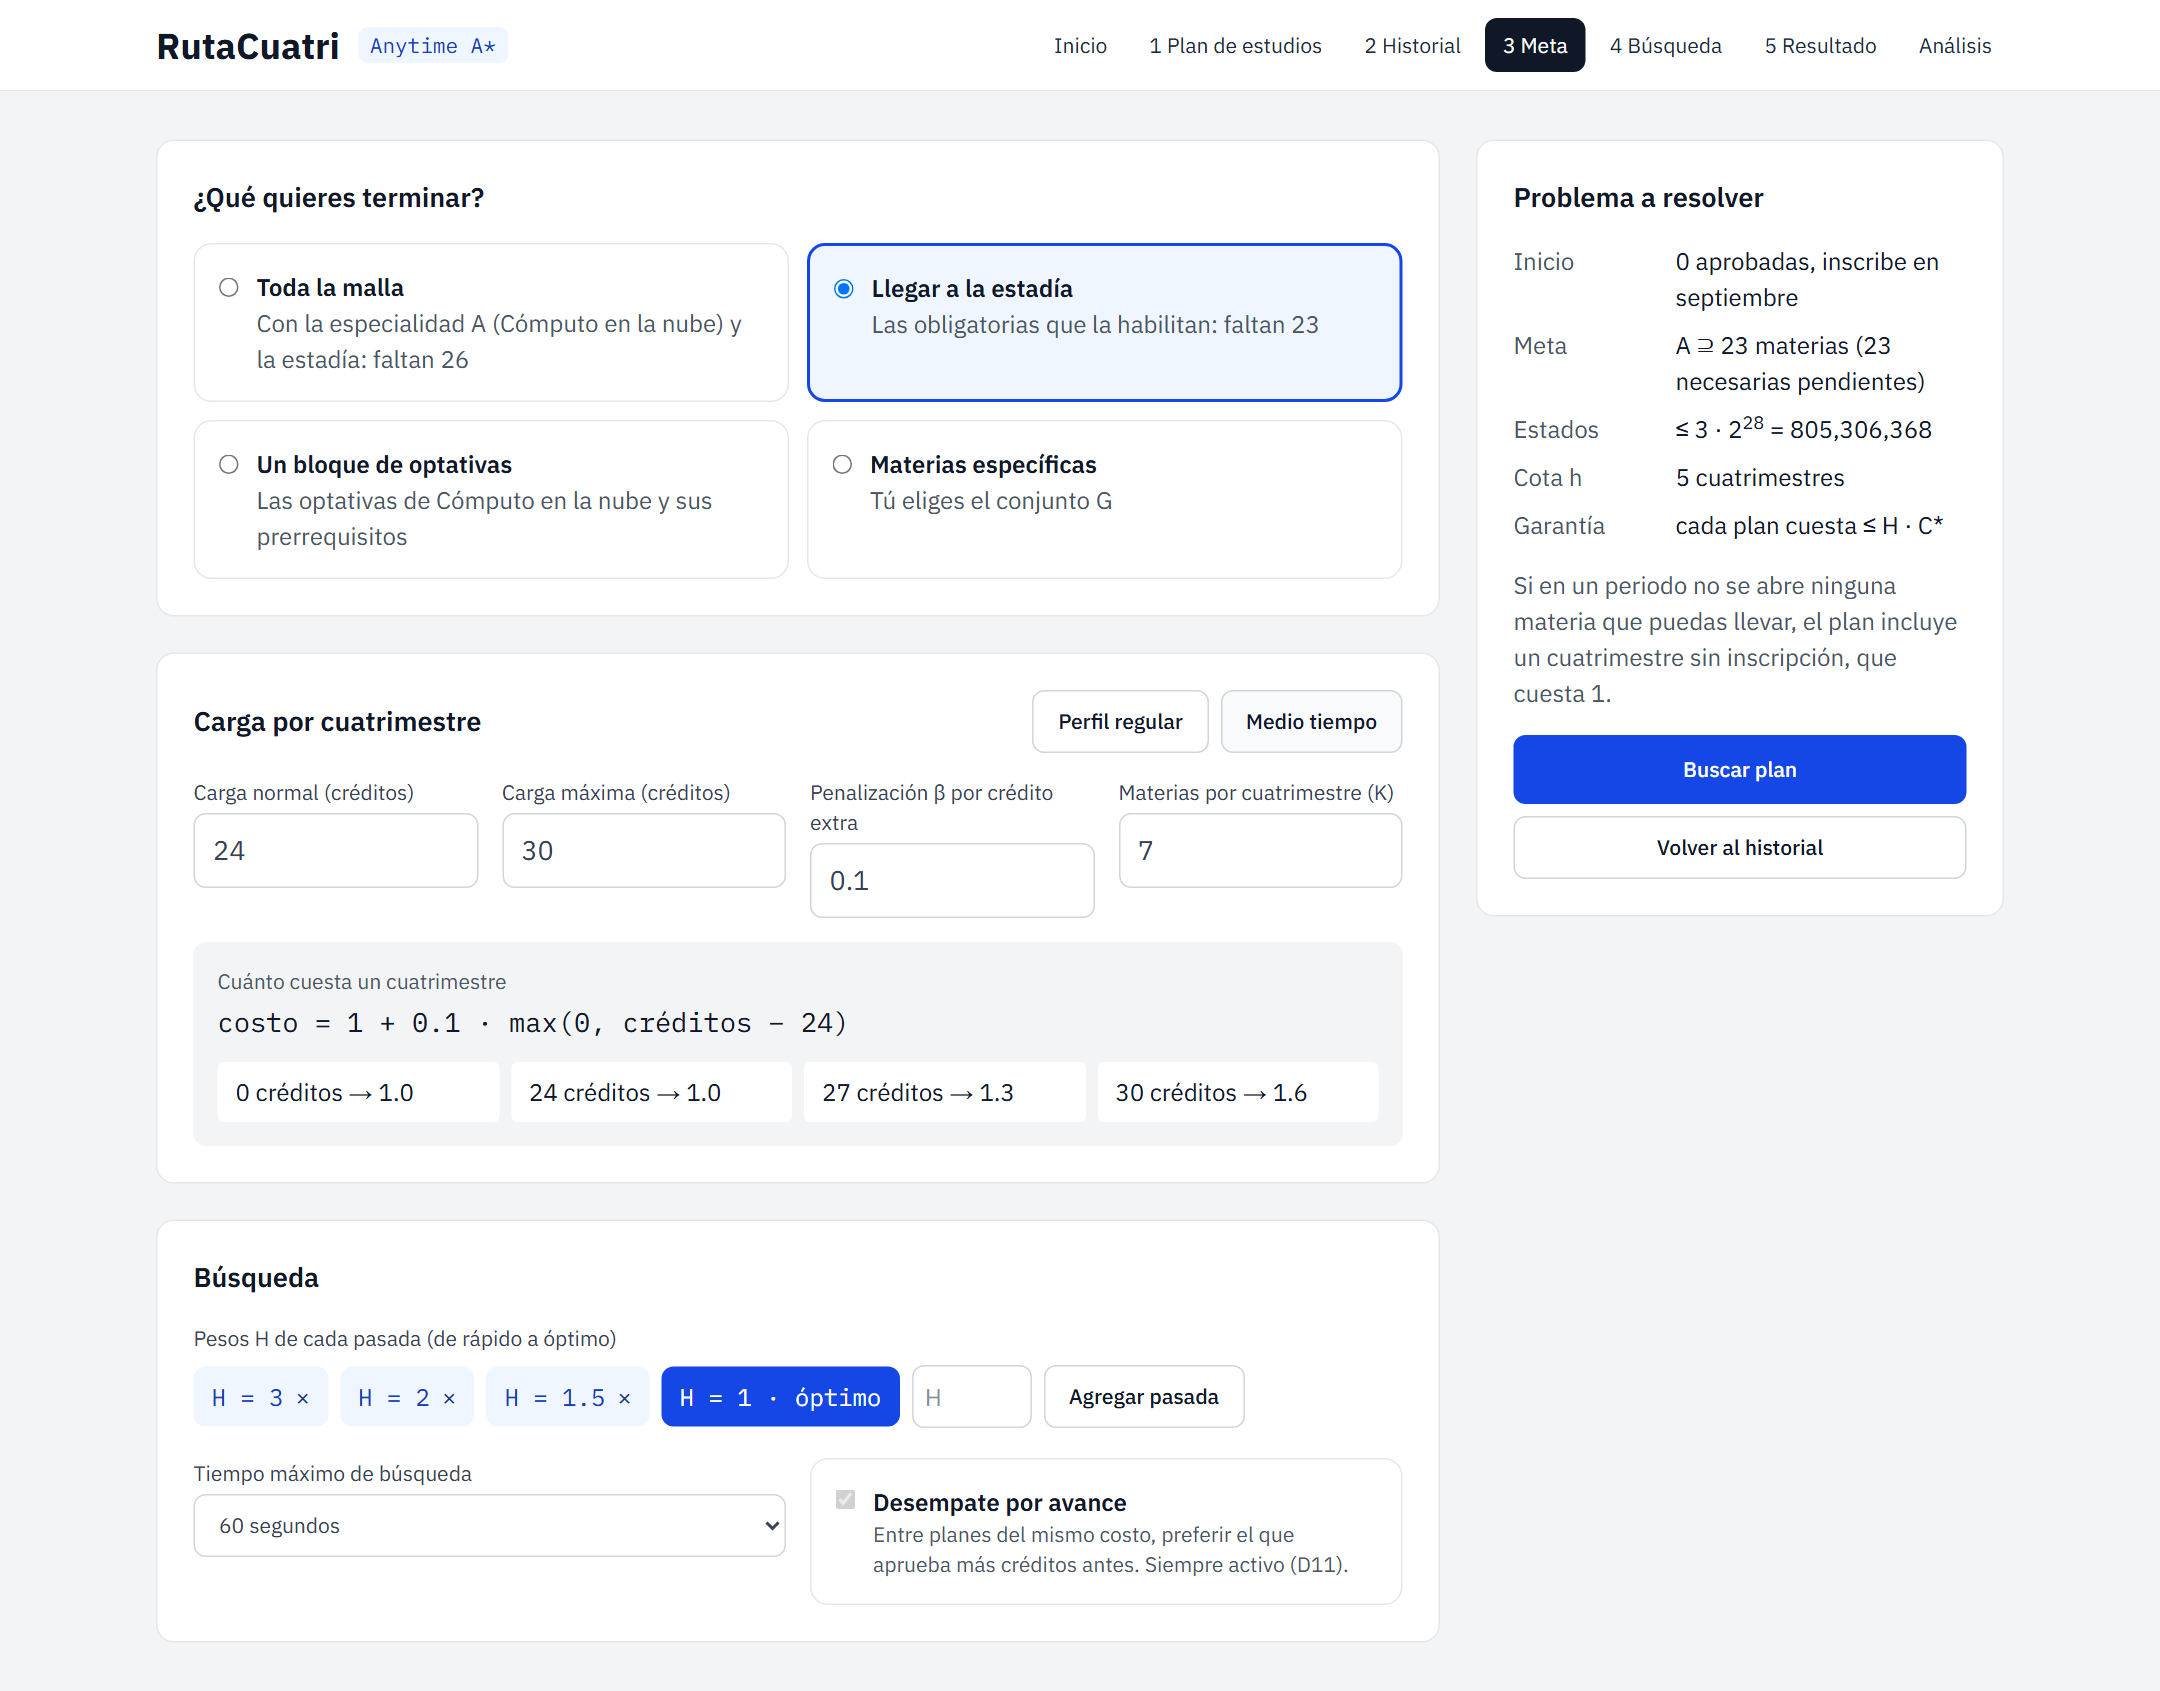
\includegraphics[width=\textwidth,height=0.75\textheight,keepaspectratio]{caso3-meta}
    \caption{Caso 3: meta ``llegar a la estadía'' con medio tiempo}
    \label{FIG::C3Meta}
\end{figure}

\subsection{Solución}
El plan óptimo tiene 6 cuatrimestres y costo 6.1 (Figura~\ref{FIG::C3Resultado}): cinco cuatrimestres sin sobrecarga y uno de 25 créditos, un crédito arriba de la carga normal.

\begin{figure}[H]
    \centering
    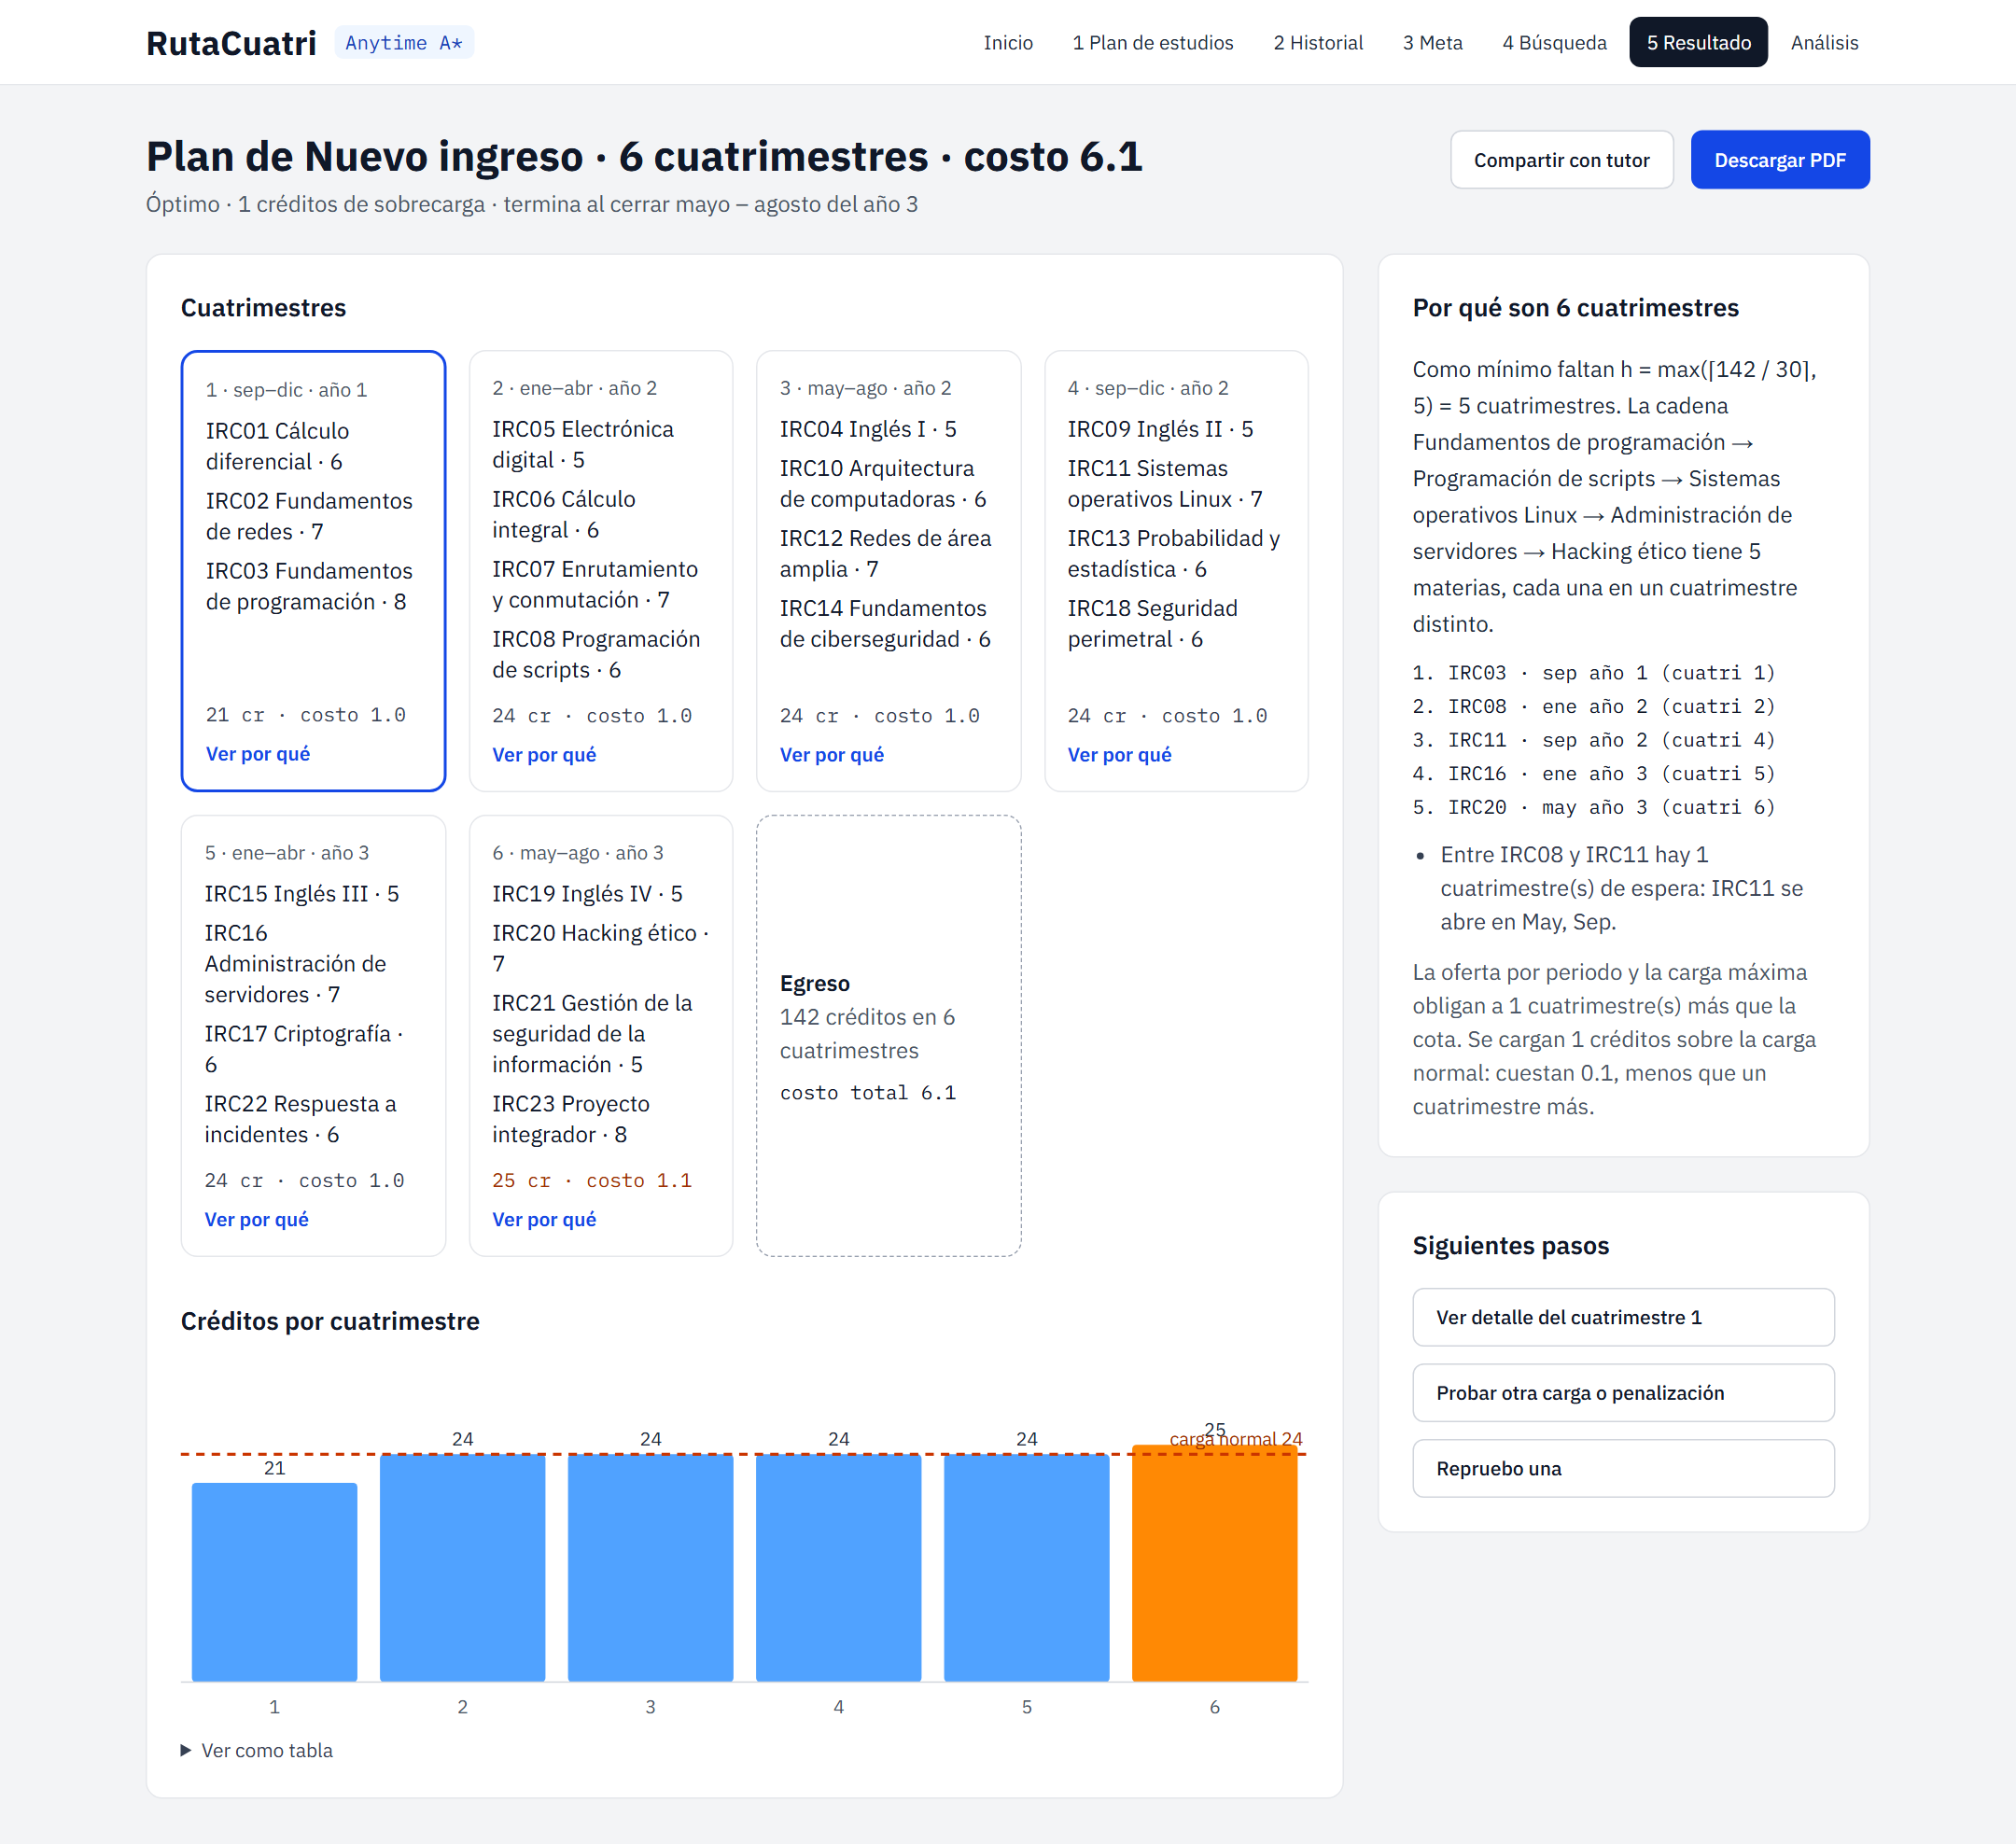
\includegraphics[width=\textwidth,height=0.75\textheight,keepaspectratio]{caso3-resultado}
    \caption{Caso 3: plan óptimo para llegar a la estadía}
    \label{FIG::C3Resultado}
\end{figure}

\subsection{Ejecución}
Las cuatro pasadas vuelven a mejorar el plan: 7.0, 6.8, 6.4 y 6.1, con 6, 10, 7 y 38 expansiones (Figura~\ref{FIG::C3Busqueda}).

\begin{figure}[H]
    \centering
    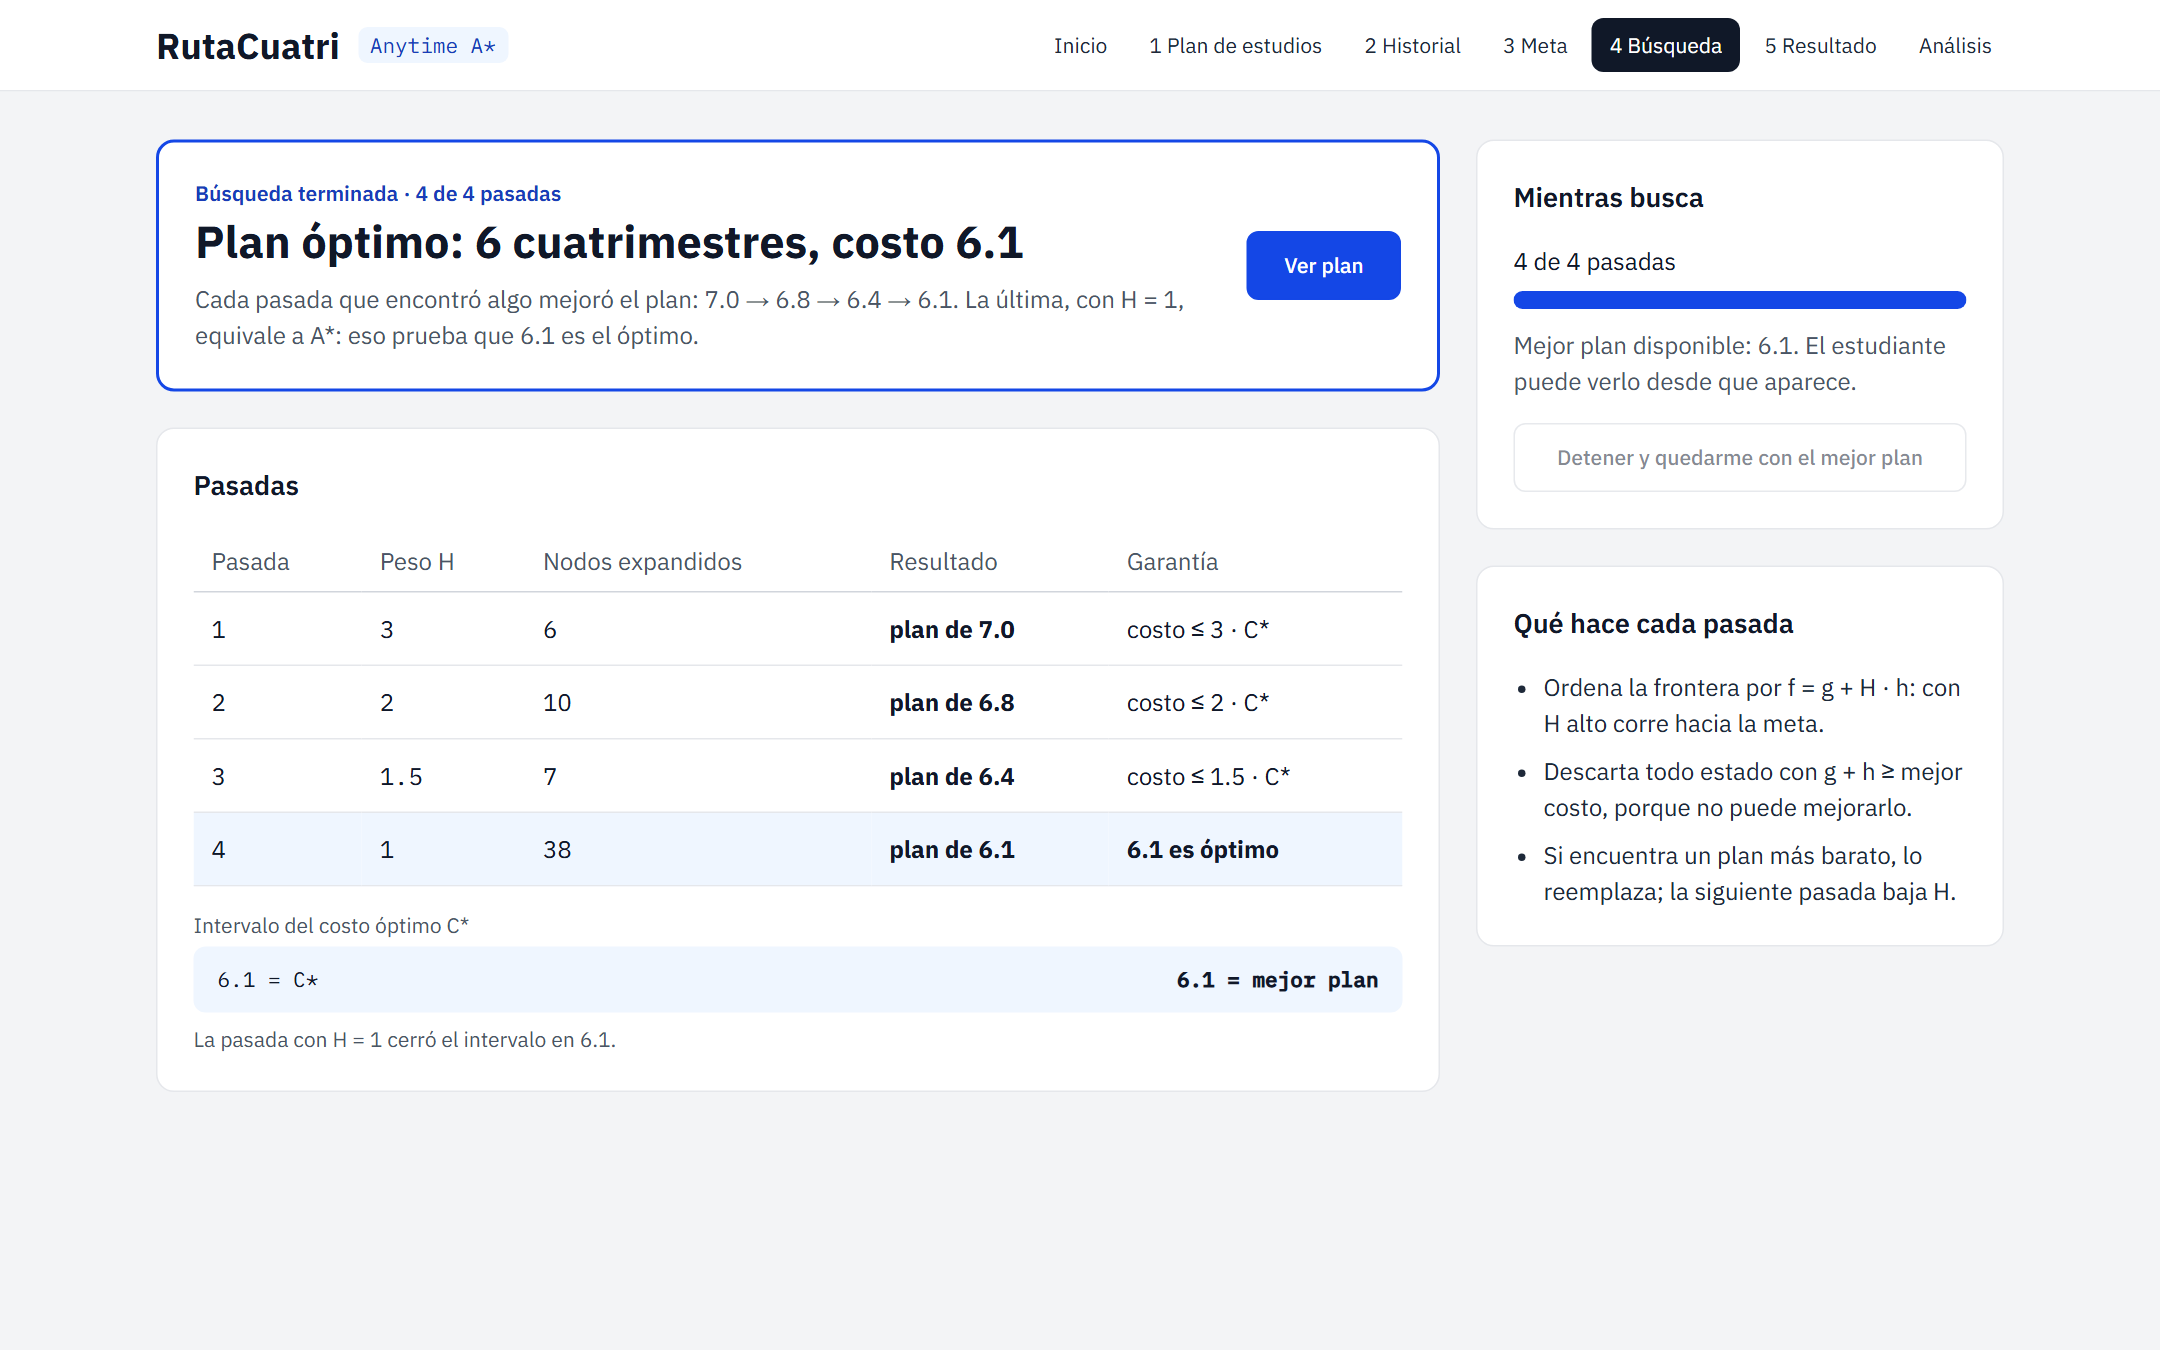
\includegraphics[width=\textwidth,height=0.75\textheight,keepaspectratio]{caso3-busqueda}
    \caption{Caso 3: pasadas de Anytime A*}
    \label{FIG::C3Busqueda}
\end{figure}

\subsection{Comentarios}
El óptimo usa un cuatrimestre más que la cota: la cadena de cinco materias pide 5, pero con 24 créditos de carga normal los 142 créditos no caben sin sobrecarga en 5 cuatrimestres. El plan acepta un solo crédito de sobrecarga, que cuesta 0.1, en lugar de un séptimo cuatrimestre. La pasada con $H = 3$ ya da un plan de 7.0, a 15\% del óptimo.

\section{Caso 4: meta imposible}

\subsection{Descripción}
Se modificó la malla ISW para que Proyecto integrador (ISW23) no se abra en ningún periodo; es el caso especial T03 de las pruebas. Como ISW23 es necesaria para la estadía y la titulación, ningún plan puede cumplir la meta M1.

\subsection{Estado inicial y meta}
El estado inicial es el de nuevo ingreso, $(\emptyset, \text{Sep})$, y la meta es M1. La Figura~\ref{FIG::C4Malla} muestra la tabla de materias con ISW23 marcada ``Sin oferta''.

\begin{figure}[H]
    \centering
    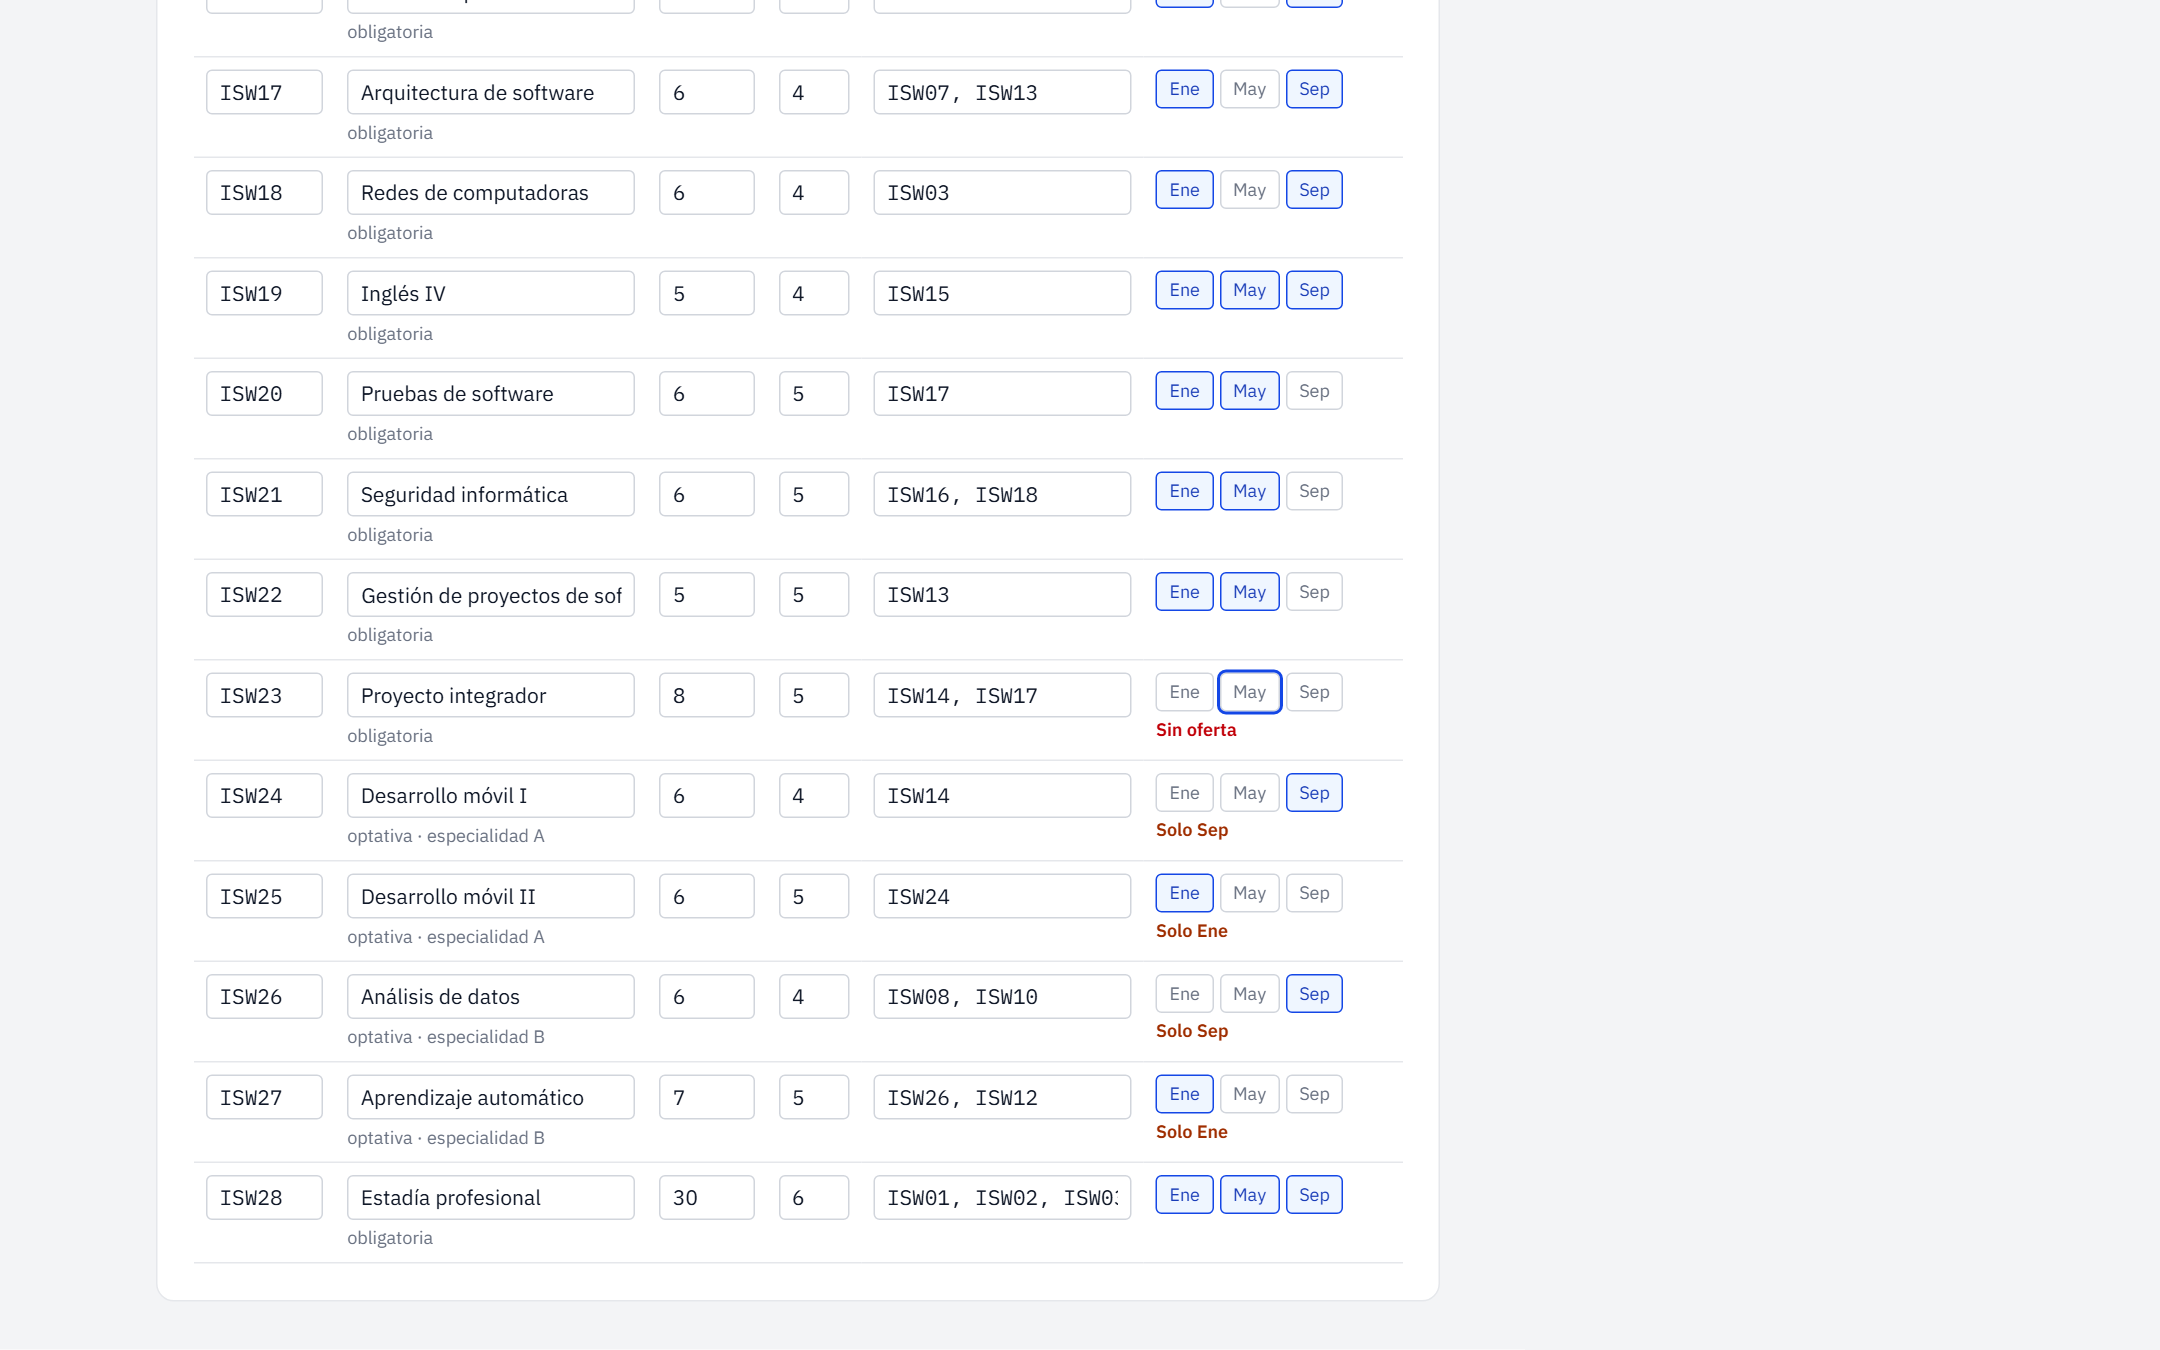
\includegraphics[width=\textwidth,height=0.75\textheight,keepaspectratio]{caso4-malla}
    \caption{Caso 4: ISW23 sin oferta en el plan de estudios}
    \label{FIG::C4Malla}
\end{figure}

\subsection{Solución}
Al presionar ``Buscar plan'', la validación detecta que una materia necesaria no se abre en ningún periodo y la interfaz va directo a la pantalla ``Sin plan posible'' sin ejecutar la búsqueda (Figura~\ref{FIG::C4SinPlan}). La pantalla muestra la causa (la materia, sus prerrequisitos y su oferta) y tres opciones: planear sin esa materia, solicitar que se abra (con un enlace para revisar su oferta en el plan de estudios) o cambiar la meta.

\begin{figure}[H]
    \centering
    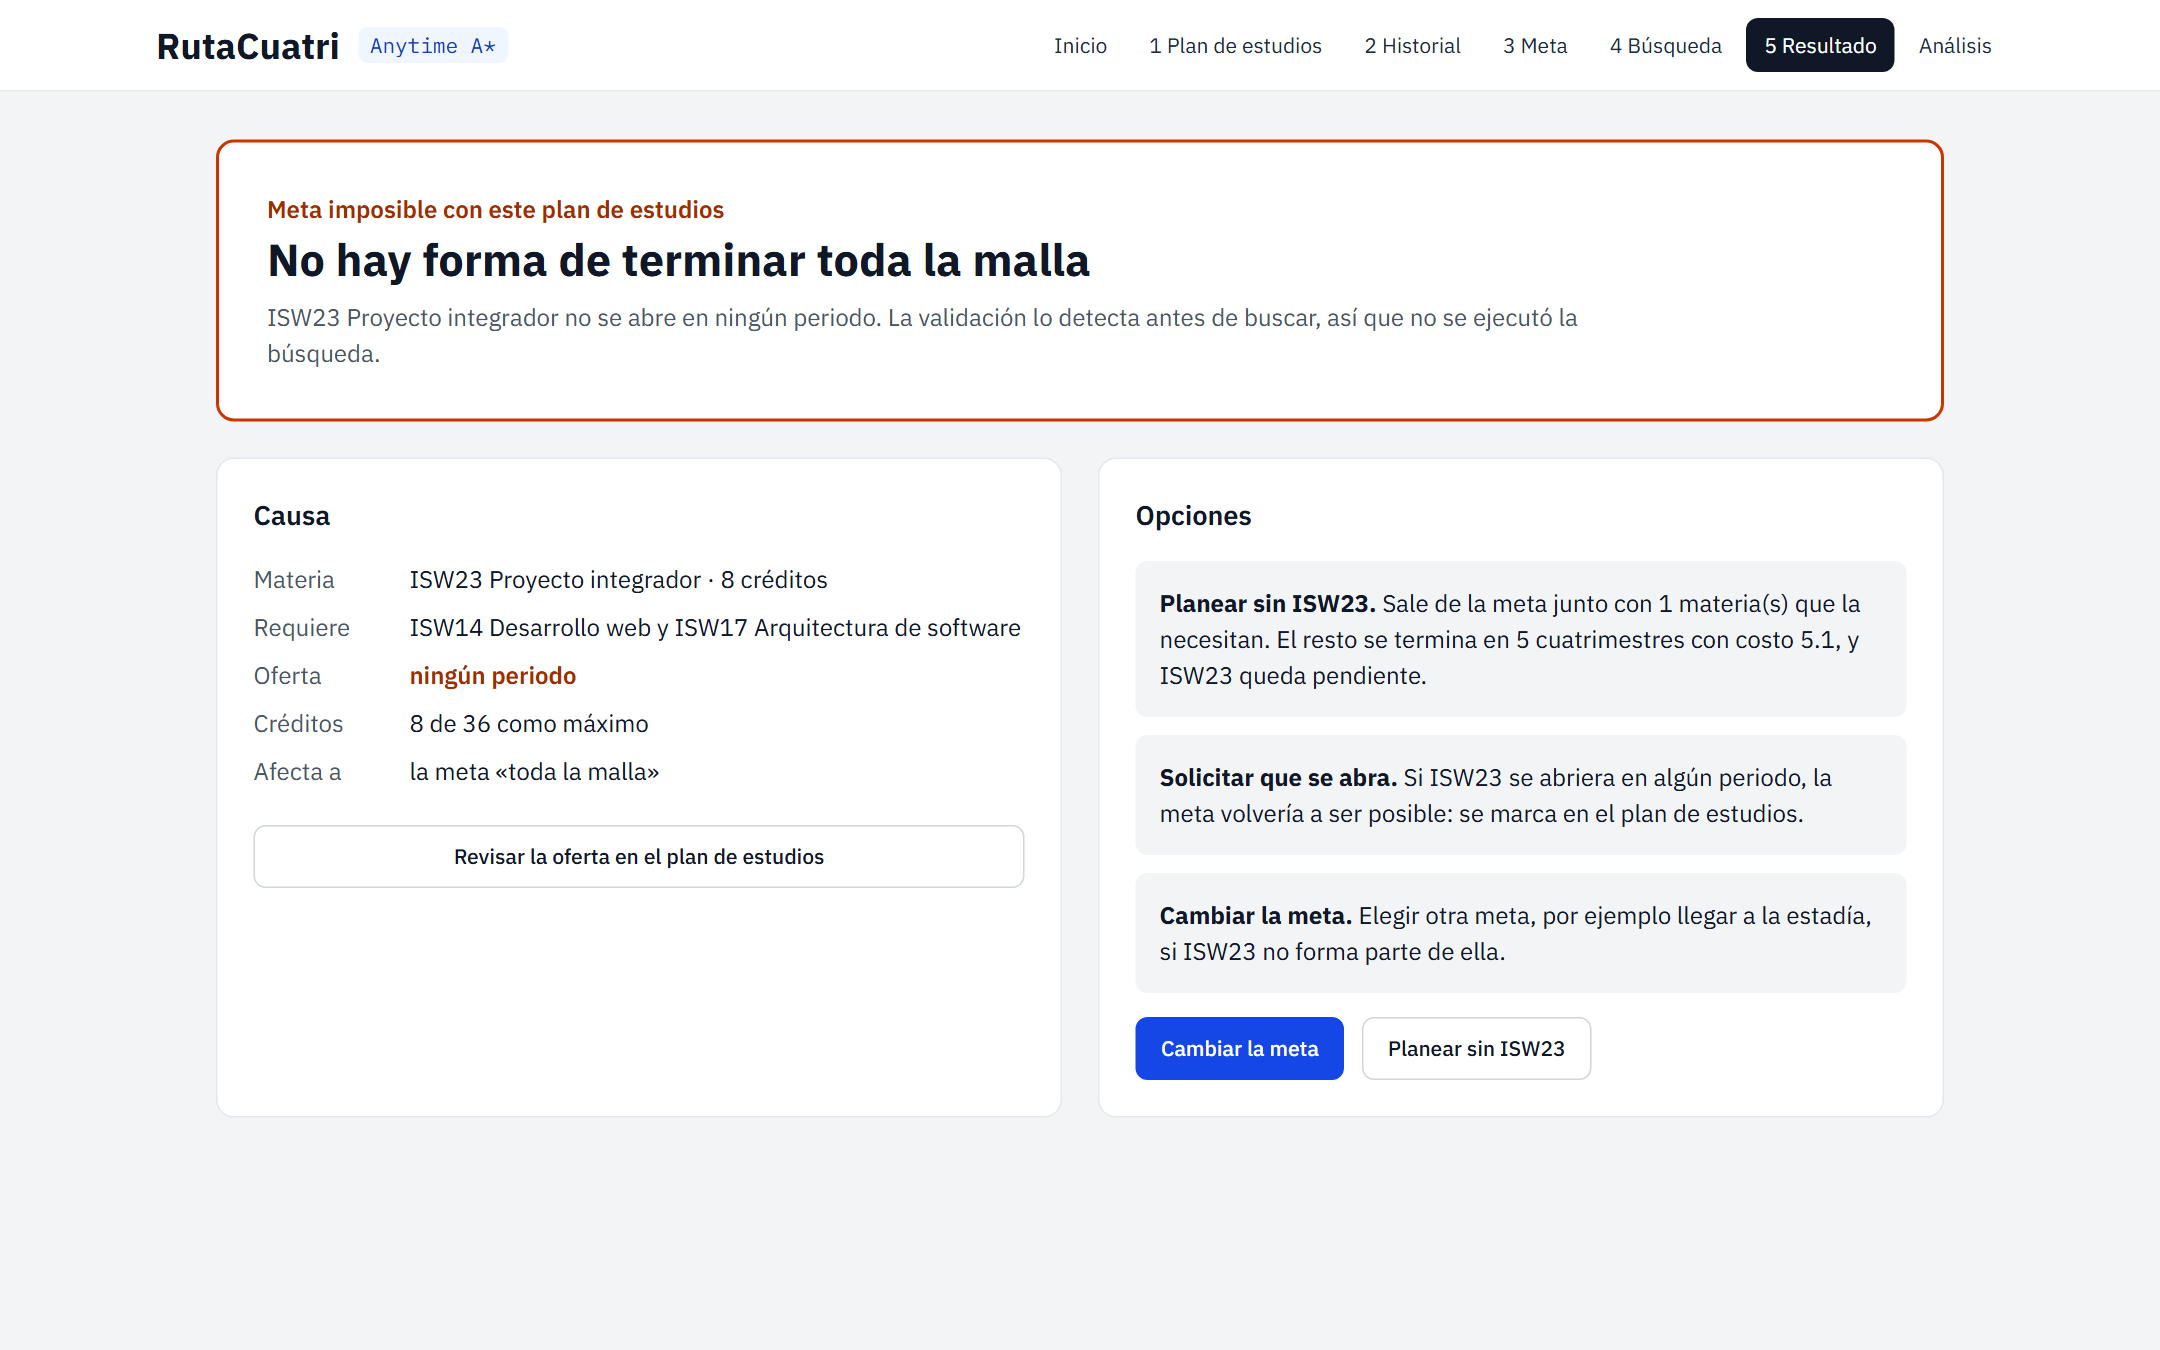
\includegraphics[width=\textwidth,height=0.75\textheight,keepaspectratio]{caso4-sin-plan}
    \caption{Caso 4: pantalla ``Sin plan posible''}
    \label{FIG::C4SinPlan}
\end{figure}

\subsection{Ejecución}
No hay pasadas: la búsqueda nunca empieza. La opción ``Planear sin ISW23'' quita de la meta a ISW23 y a la estadía, que la necesita, y calcula con A* el plan del resto: 24 materias en 5 cuatrimestres con costo 5.1.

\subsection{Comentarios}
Validar antes de buscar evita una búsqueda inútil: sin la validación, la búsqueda tendría que agotar todo el espacio alcanzable para concluir que no hay plan. Como las reglas de la validación garantizan que, si pasan, siempre existe un plan, la pantalla ``Sin plan posible'' sale solo de la validación.

\section{Experimentos}
Los cuatro experimentos se corren con el script \texttt{scripts/experimento.ts}, que usa el mismo motor en Node y escribe un archivo CSV por experimento. Cada corrida se repite 5 veces y se reporta la mediana del tiempo; los costos y las expansiones no cambian entre repeticiones. Una corrida se corta a los 60 s, pero ninguna llegó a ese límite.

\subsection{Experimento A: primer plan y óptimo}
Se corrió Anytime A* en los 72 escenarios. En los 72 el costo final coincide con el óptimo esperado y cada pasada cumple $\text{costo} \leq H \cdot C^*$. En 52 de los 72 escenarios la primera pasada ya da el plan óptimo (27 de 36 con el perfil regular y 25 de 36 con medio tiempo). El peor primer plan es el de Daniel Ortega en ICD con la meta M1: 6.1 contra un óptimo de 4.3, es decir, 1.42 veces el óptimo, muy por debajo de la garantía de 3. La mediana del tiempo hasta el primer plan es de 0.04 ms y la del tiempo total de 0.08 ms; el escenario más largo es el Caso 2, con 38.6 ms.

La Figura~\ref{FIG::ExpA} muestra el costo del mejor plan contra las expansiones acumuladas en el Caso 2: el plan baja de 10.0 a 8.5 y casi todo el trabajo está en la última pasada.

\begin{figure}[H]
    \centering
    \begin{tikzpicture}
        \begin{semilogxaxis}[
            width=0.9\textwidth, height=7cm,
            xlabel={Expansiones acumuladas (escala logarítmica)},
            ylabel={Costo del mejor plan},
            ymin=7.5, ymax=10.5,
            xmin=10, xmax=10000,
            grid=major,
        ]
            \addplot[const plot, thick, blue, mark=*,
                nodes near coords, point meta=explicit symbolic,
                every node near coord/.append style={font=\footnotesize, anchor=south west, fill=white, inner sep=1pt, xshift=2pt, yshift=2pt}] coordinates {
                (17,10.0)[$H=3$: 10.0]
                (39,9.6)[$H=2$: 9.6]
                (116,8.8)[$H=1.5$: 8.8]
                (3034,8.5)[$H=1$: 8.5]
            };
            \addplot[dashed, gray] coordinates {(10,8.5) (10000,8.5)};
        \end{semilogxaxis}
    \end{tikzpicture}
    \caption{Experimento A: costo contra expansiones acumuladas de Anytime A*, ISW-E1, meta M1, medio tiempo. La línea punteada es el óptimo.}
    \label{FIG::ExpA}
\end{figure}

\subsection{Experimento B: comparación de métodos}
Se compararon Anytime A*, A*, Weighted A* con $H = 2$ y Costo Uniforme en los 24 escenarios con meta M1. La Tabla~\ref{TAB::ExpB} y la Figura~\ref{FIG::ExpB} resumen los resultados.

\begin{table}[H]
  \begin{center}
    \caption{Experimento B: 24 escenarios con meta M1}
    \label{TAB::ExpB}
    \begin{tabular}{|| l | r | c | r ||}
        \hline
        Método & Expansiones totales & Óptimos & Primer plan, medio tiempo \\ [0.5ex]
        \hline\hline
        Anytime A* & 7,197 & 24 / 24 & 0.05 ms \\
        \hline
        A* & 5,523 & 24 / 24 & 0.23 ms \\
        \hline
        Weighted A* ($H = 2$) & 270 & 11 / 24 & 0.07 ms \\
        \hline
        Costo Uniforme & 10,452 & 24 / 24 & 0.17 ms \\
        \hline
    \end{tabular}
  \end{center}
\end{table}

\begin{figure}[H]
    \centering
    \begin{tikzpicture}
        \begin{axis}[
            xbar, width=0.72\textwidth, height=6cm,
            xlabel={Nodos expandidos en los 24 escenarios},
            ytick={1,2,3,4},
            yticklabels={Weighted A* ($H=2$), A*, Anytime A*, Costo Uniforme},
            xmin=0, xmax=12500,
            nodes near coords,
            nodes near coords align={horizontal},
            bar width=14pt,
            enlarge y limits=0.2,
        ]
            \addplot[fill=blue!60] coordinates {(270,1) (5523,2) (7197,3) (10452,4)};
        \end{axis}
    \end{tikzpicture}
    \caption{Experimento B: expansiones por método}
    \label{FIG::ExpB}
\end{figure}

Costo Uniforme es óptimo pero, sin heurística, expande casi el doble que A*. Weighted A* con $H = 2$ expande muy poco pero solo da el óptimo en 11 de 24 casos. Anytime A* expande 30\% más que A* porque repite la búsqueda en cada pasada, y a cambio entrega un plan desde la primera pasada y siempre llega al óptimo.

\subsection{Experimento C: reglas de poda}
Se corrió A* con y sin las reglas de generación de sucesores (solo materias necesarias, poda por dominancia y cuatrimestre vacío solo si no hay nada) para los estudiantes E1 y E3, con la meta M1 y medio tiempo. La Tabla~\ref{TAB::ExpC} muestra que el costo es el mismo en los seis casos y que las reglas reducen las expansiones entre 2.3 y 18.9 veces.

\begin{table}[H]
  \begin{center}
    \caption{Experimento C: nodos expandidos por A* con y sin las reglas}
    \label{TAB::ExpC}
    \begin{tabular}{|| l | c | r | r | r ||}
        \hline
        Estudiante & Costo & Sin reglas & Con reglas & Ahorro \\ [0.5ex]
        \hline\hline
        ISW-E1 & 8.5 & 8,644 & 2,918 & 3.0 \\
        \hline
        ISW-E3 & 6.6 & 2,453 & 1,084 & 2.3 \\
        \hline
        IRC-E1 & 8.6 & 1,423 & 393 & 3.6 \\
        \hline
        IRC-E3 & 7.6 & 450 & 33 & 13.6 \\
        \hline
        ICD-E1 & 8.5 & 2,807 & 574 & 4.9 \\
        \hline
        ICD-E3 & 7.6 & 284 & 15 & 18.9 \\
        \hline
    \end{tabular}
  \end{center}
\end{table}

\subsection{Experimento D: qué parámetro decide el egreso}
Se corrió A* para el nuevo ingreso de ISW con la meta M1, cambiando un solo parámetro del perfil regular cada vez (Tabla~\ref{TAB::ExpD}).

\begin{table}[H]
  \begin{center}
    \caption{Experimento D: sensibilidad para ISW-E1, meta M1}
    \label{TAB::ExpD}
    \begin{tabular}{|| l | c | c | c ||}
        \hline
        Cambio sobre el perfil regular & Costo & Cuatrimestres & Créditos de sobrecarga \\ [0.5ex]
        \hline\hline
        Ninguno & 6.4 & 6 & 4 \\
        \hline
        $\beta = 0.05$ & 6.2 & 6 & 4 \\
        \hline
        $\beta = 0.2$ & 6.8 & 6 & 4 \\
        \hline
        $\beta = 0.5$ & 7.0 & 7 & 0 \\
        \hline
        $C_{norm} = 24$ & 8.5 & 7 & 15 \\
        \hline
        $C_{norm} = 27$ & 7.4 & 7 & 4 \\
        \hline
        $C_{norm} = 33$ & 6.0 & 6 & 0 \\
        \hline
        $C_{max} = 30$ & 7.0 & 7 & 0 \\
        \hline
        $C_{max} = 33$ o $40$ & 6.4 & 6 & 4 \\
        \hline
        $K = 5$ o $6$ & 6.4 & 6 & 4 \\
        \hline
    \end{tabular}
  \end{center}
\end{table}

La carga normal es la que más mueve el egreso: con $C_{norm} = 24$ el plan pasa a 7 cuatrimestres y aun así carga 15 créditos de más. Subir la carga máxima arriba de 33 no adelanta nada, porque lo que manda es la cadena de seriación. Con $\beta = 0.5$ conviene un séptimo cuatrimestre antes que cargar de más. Los doce valores coinciden con los de la implementación de referencia. La pantalla de análisis repite este experimento para cualquier escenario (Anexo~\ref{ANX::Analisis}).
\clearpage
\chapter{Conclusiones y recomendaciones}

\section{Conclusiones}
El proyecto cumplió su objetivo: dado un plan de estudios, un historial y una meta, RutaCuatri entrega el plan de inscripción de menor costo y demuestra que no existe uno mejor. En los 72 escenarios la pasada con $H = 1$ terminó y su costo coincidió con el de la implementación de referencia, y en todas las pasadas se cumplió la garantía $\text{costo} \leq H \cdot C^*$.

\textbf{Qué se aprendió.} La parte decisiva no fue el algoritmo de búsqueda sino el modelo. Representar el estado como (materias aprobadas, periodo) hizo que el problema cupiera en un entero de 32 bits; restringir los sucesores a las materias necesarias y descartar los conjuntos dominados redujo las expansiones hasta 19 veces sin perder el óptimo (Tabla~\ref{TAB::ExpC}), y una heurística consistente permitió cerrar los estados sin reabrirlos. También se aprendió a comprobar un buscador: compararlo con una implementación de referencia independiente, revisar cada plan con un verificador aparte y probar propiedades en mallas al azar da una confianza que un solo caso de ejemplo no da. Las pruebas en el navegador, por su parte, encontraron un error de la vista de celular que en escritorio no se veía.

Sobre el método, Anytime A* se comportó como se esperaba: en el Caso 2 dio un primer plan a 18\% del óptimo con menos del 1\% de las expansiones de A*, y en 52 de los 72 escenarios la primera pasada ya era óptima. El costo de esa ventaja es repetir la búsqueda: en total expandió 30\% más nodos que A* (Tabla~\ref{TAB::ExpB}). Con mallas de 28 materias todo termina en milisegundos, así que la ventaja práctica de Anytime crece con mallas más grandes o con cargas que obligan a negociar entre sobrecarga y cuatrimestres.

Para el estudiante, el experimento D deja una conclusión útil: la carga normal es lo que más decide cuándo egresa, mientras que subir la carga máxima arriba de 33 créditos no adelanta nada, porque lo que manda es la cadena de seriación.

\textbf{Qué se haría diferente.} Se definirían desde el principio los casos de prueba con respuesta conocida, antes de escribir el motor: fueron la herramienta que más ahorró tiempo. También se diseñaría la heurística con un tercer término, por ejemplo la espera mínima hasta el siguiente periodo en que se abre la primera materia de la cadena crítica, porque en varios escenarios la cota inicial queda un cuatrimestre por debajo del óptimo por la oferta, y una cota más ajustada reduciría la última pasada.

\textbf{Nuevos proyectos.} El mismo modelo sirve para planear con varios escenarios de oferta (por ejemplo, la probabilidad de que un grupo se abra), lo que lo convertiría en un problema no determinista; para recomendar a la coordinación qué materias abrir en cada periodo según los planes de todos los estudiantes irregulares, y para combinarlo con un generador de horarios que reciba las materias de cada cuatrimestre.

\section{Recomendaciones}
\begin{itemize}
    \item \textbf{Mallas más grandes.} El estado como entero de 32 bits limita la malla a 31 materias. Para una carrera completa de 60 materias habría que pasar a dos enteros o a \texttt{BigInt}, y medir de nuevo el tiempo, porque ahí la ventaja de Anytime A* frente a A* sería mayor.
    \item \textbf{Reutilizar la frontera entre pasadas.} Cada pasada empieza desde cero. Una variante tipo ARA* \cite{likhachev2003}, que reutiliza la frontera y reabre estados, ahorraría expansiones en mallas grandes, a cambio de un código más difícil de probar.
    \item \textbf{Datos oficiales.} Las mallas son de diseño propio. Integrar los planes y la oferta oficiales de la universidad, por ejemplo con un importador desde el sistema escolar, haría que el sistema se pudiera usar en la tutoría real.
    \item \textbf{Materias reprobadas con probabilidad.} Hoy una materia reprobada se modela volviendo a planear. Un modelo que considere la probabilidad de reprobar podría preferir planes con margen.
\end{itemize}
\clearpage
\chapter{Anexos}

\section{Pantalla de análisis de escenarios}
\label{ANX::Analisis}
La pantalla de análisis (Figura~\ref{FIG::Analisis}) repite la búsqueda cambiando un solo parámetro por fila ($\beta$, $C_{norm} \pm 3$ y $C_{max}$ de 30, 33 y 40) y compara Anytime A*, A*, Weighted A* con $H = 2$ y Costo Uniforme sobre el escenario actual. Es la versión interactiva de los experimentos B y D del Capítulo~\ref{CAP::Resultados}. La figura corresponde al escenario de Ana Ruiz (Caso 1).

\begin{figure}[H]
    \centering
    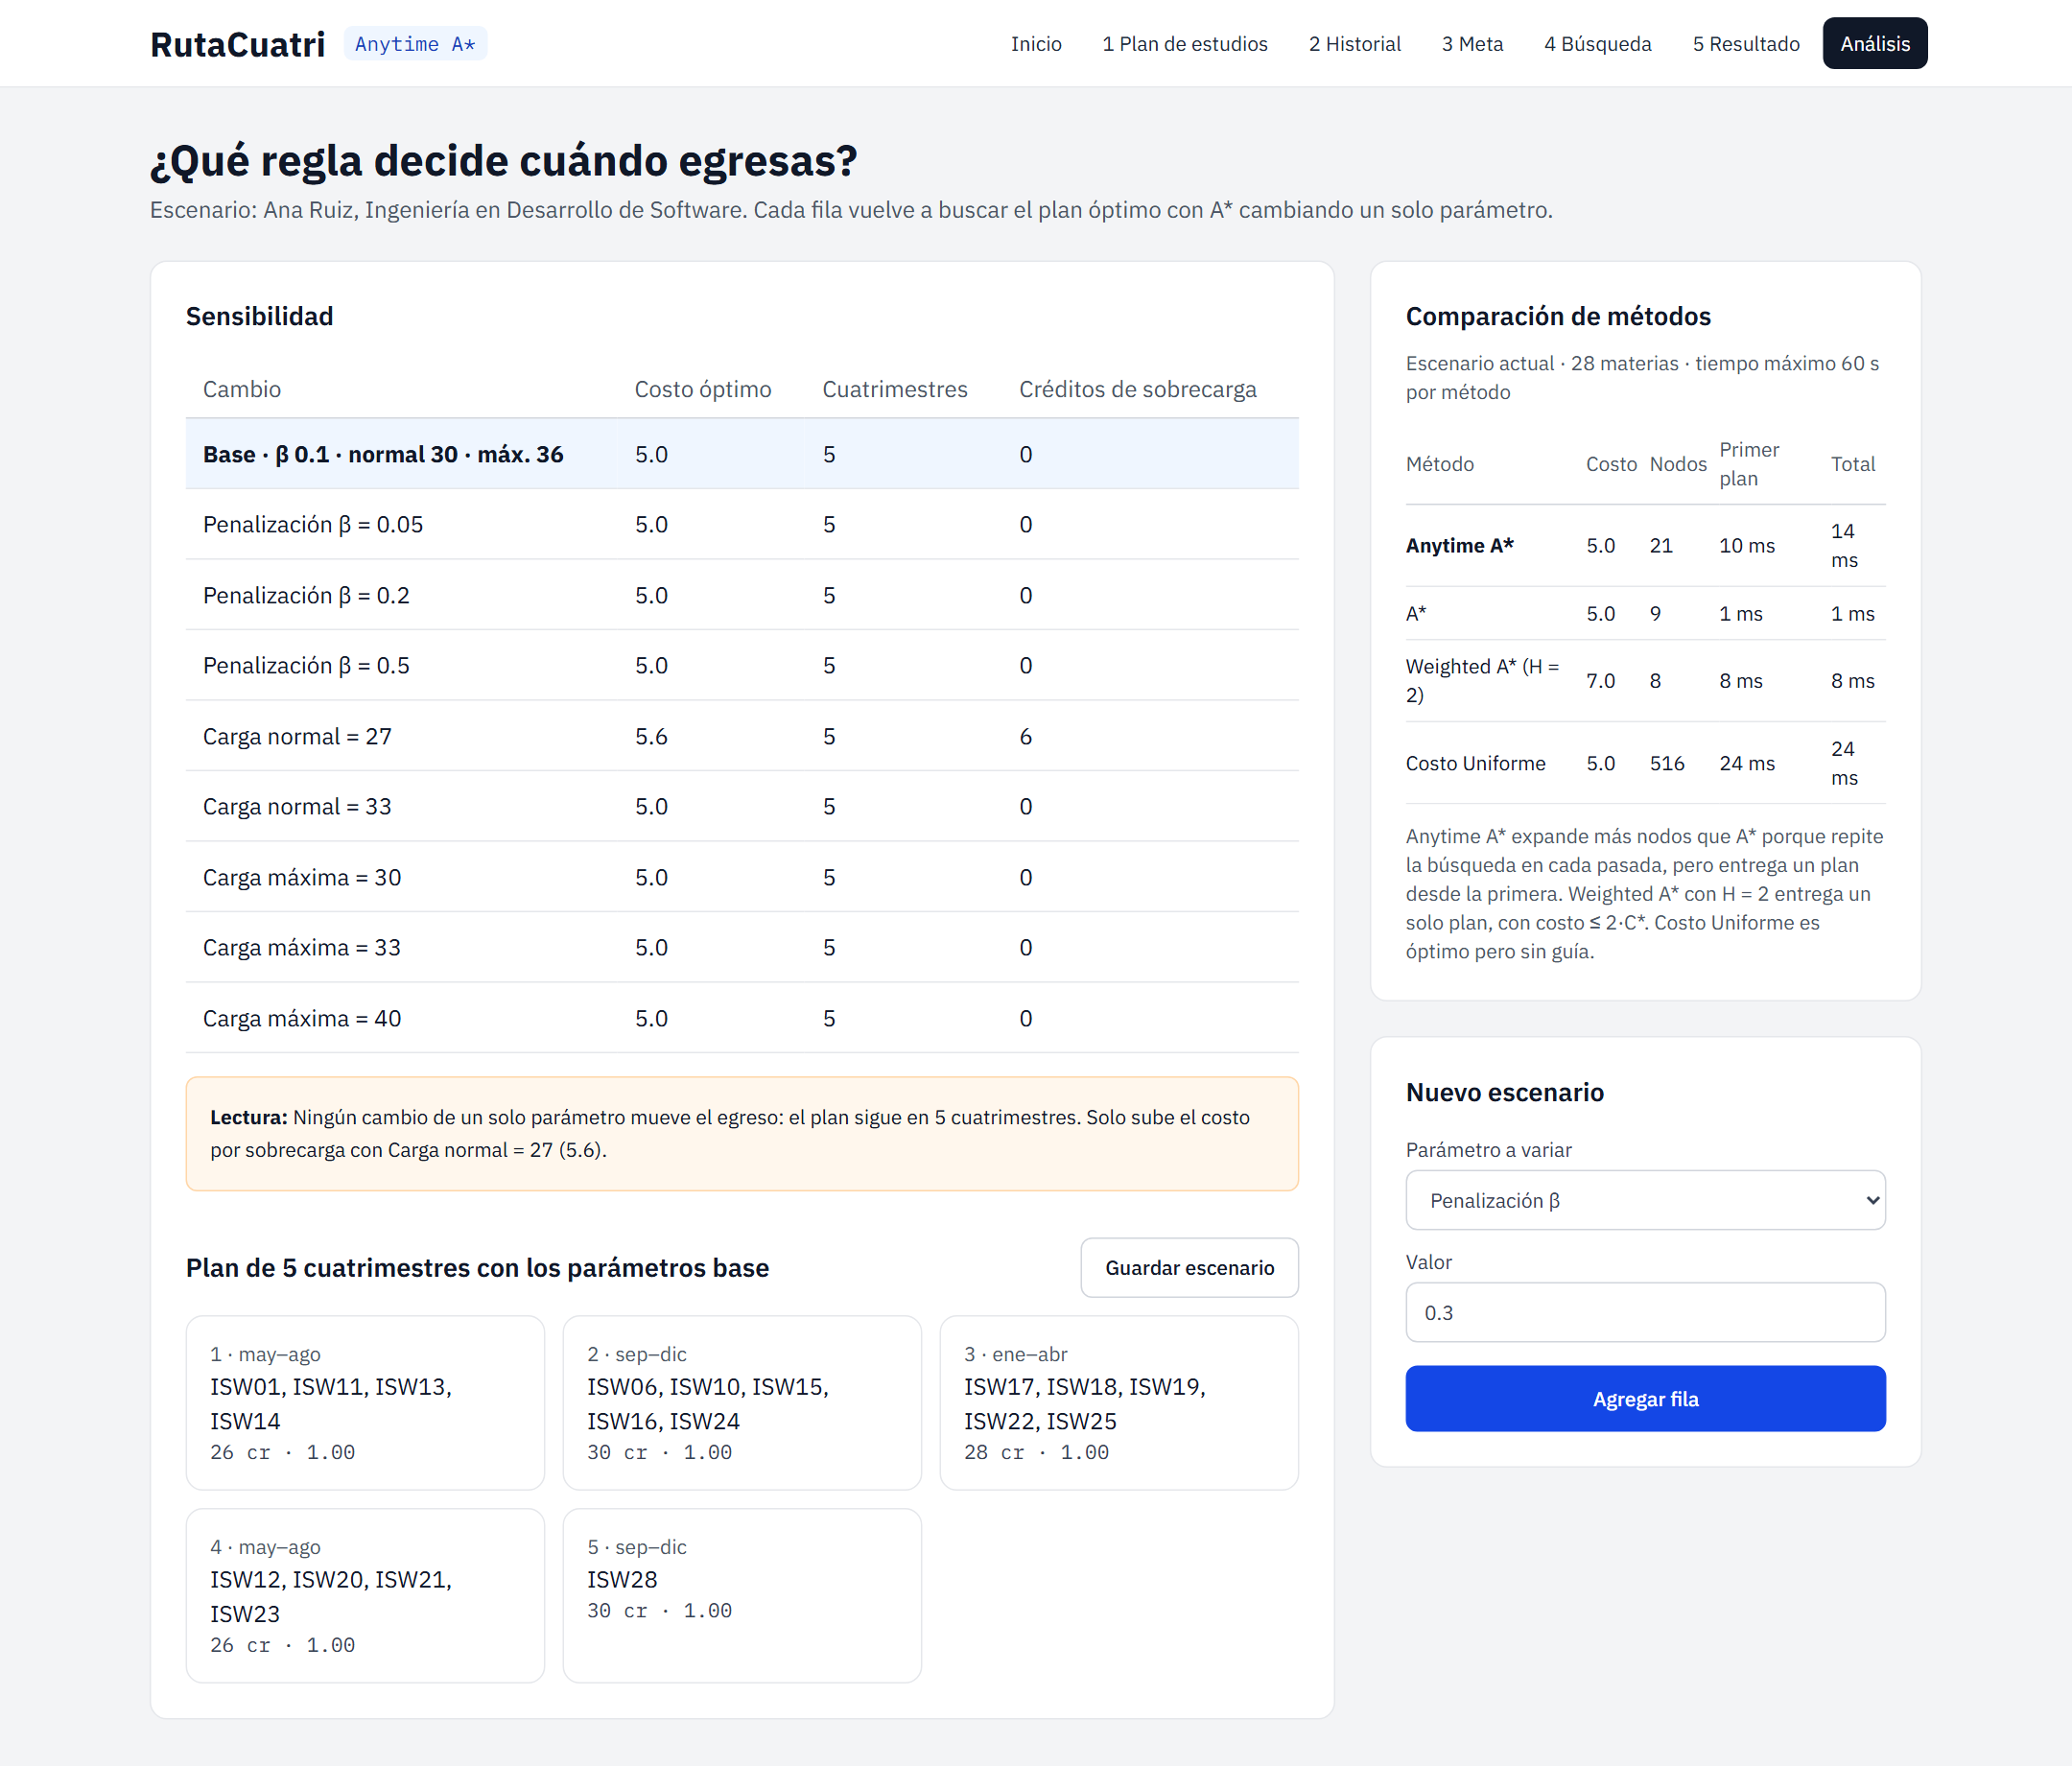
\includegraphics[width=\textwidth,height=0.8\textheight,keepaspectratio]{caso1-analisis}
    \caption{Pantalla de análisis de escenarios para el Caso 1}
    \label{FIG::Analisis}
\end{figure}

\section{Repositorio y ejecución}
\label{ANX::Repositorio}
El código está en \url{https://github.com/lsprz2773/RutaCuatri}. La Tabla~\ref{TAB::Carpetas} resume las carpetas y la Tabla~\ref{TAB::Comandos} los comandos; requiere Node 22.18 o superior.

\begin{table}[H]
  \begin{center}
    \caption{Carpetas del repositorio}
    \label{TAB::Carpetas}
    \begin{tabular}{|| p{5cm} | p{8.5cm} ||}
        \hline
        Carpeta & Contenido \\ [0.5ex]
        \hline\hline
        \texttt{src/motor} & Método de búsqueda (Capítulo 2) \\
        \hline
        \texttt{src/worker} & Web Worker que ejecuta el motor en el navegador \\
        \hline
        \texttt{src/app}, \texttt{src/componentes}, \texttt{src/estado} & Interfaz: las diez pantallas y su estado \\
        \hline
        \texttt{public/datos} & Las tres mallas, los alumnos tipo y las metas en JSON \\
        \hline
        \texttt{pruebas} & 77 casos de prueba, verificador, pruebas de propiedad y flujos de Playwright \\
        \hline
        \texttt{scripts} & Experimentos, implementación de referencia en Python y capturas \\
        \hline
        \texttt{resultados} & CSV de los experimentos A a D y datos del equipo \\
        \hline
    \end{tabular}
  \end{center}
\end{table}

\begin{table}[H]
  \begin{center}
    \caption{Comandos principales}
    \label{TAB::Comandos}
    \begin{tabular}{|| l | p{8cm} ||}
        \hline
        Comando & Qué hace \\ [0.5ex]
        \hline\hline
        \texttt{npm install} & Instala las dependencias \\
        \hline
        \texttt{npm run dev} & Abre la aplicación en \texttt{localhost:3000} \\
        \hline
        \texttt{npm test} & Corre las pruebas del motor \\
        \hline
        \texttt{npm run experimento} & Corre los experimentos A a D y escribe los CSV \\
        \hline
        \texttt{npm run build} y \texttt{npm run e2e} & Construye el sitio estático y corre Playwright \\
        \hline
    \end{tabular}
  \end{center}
\end{table}
\clearpage


\bibliographystyle{plain}
\bibliography{referencias.bib}
\backmatter
\end{document}
